\documentclass[12pt, oneside, smallheadings]{scrbook}

\usepackage[a4paper, reset, left=35mm,right=15mm, lines=46]{geometry}
\usepackage[utf8]{inputenc} % Umlaute ermöglichen
\usepackage[T1]{fontenc}
\usepackage[ngerman]{babel} % deutsche Silbentrennung
\usepackage[numbers,square]{natbib}
\usepackage{graphicx} % Grafiken
\usepackage[printonlyused]{acronym}
\usepackage{listings, marvosym}
\usepackage[hyphens]{url}
\usepackage{breakurl}
\usepackage{tabularx}
\usepackage{longtable}
\usepackage{tabu}
\usepackage{array}
%%\usepackage{booktabs}
\usepackage{todonotes}
\usepackage{xcolor}
\usepackage{subfigure} 
\usepackage{rotating}
\usepackage{multirow}
\usepackage{enumitem}
%\usepackage{dirtree}
\usepackage{textcomp}
\usepackage[htt]{hyphenat}
\usepackage[absolute]{textpos}

\definecolor{lbcolor}{rgb}{0.95,0.95,0.95}

\usepackage{minted}

\newcolumntype{R}[1]{>{\raggedleft\arraybackslash}p{#1}}                                                                                                                                                              
\newcolumntype{L}[1]{>{\raggedright\arraybackslash}p{#1}}                    

\usepackage[hidelinks]{hyperref}

\usepackage{bookmark}

\graphicspath{{img/}}
\makeatletter
\def\maxwidth#1{\ifdim\Gin@nat@width>#1 #1\else\Gin@nat@width\fi}
\makeatother

%%% underline text with linebreak
\usepackage[normalem]{ulem}

%%% Textart
\RequirePackage{lmodern}
\fontfamily{ptm}

%%% Zeilenabstand
\RequirePackage{setspace}  
\onehalfspacing

%%% reduce linespacing in enumerations
\usepackage{enumitem}
\setlist{nosep}

%%% Kopfzeile / Fußzeile
\RequirePackage[automark]{scrpage2}
\pagestyle{scrheadings}
\renewcommand\chaptermark[1]{
    \markboth{Kapitel \thechapter: #1}{}
}
\renewcommand\sectionmark[1]{
    \markright{#1}
}
\clearscrheadfoot
\setheadsepline{0.4pt}
\ihead{\footnotesize\textnormal\leftmark}
\chead{}
\ohead{\footnotesize\textnormal\rightmark}

\ifoot{}
\cfoot[\pagemark]{\textnormal{\thepage}}
\ofoot{}
%%% Ende Kopfzeile / Fußzeile

%%% Referenzen
\RequirePackage{prettyref}
\RequirePackage{titleref}

% Kapitel
\newrefformat{chap}{siehe Kapitel \ref{#1}, Seite \pageref{#1}}
% Abschnitte
\newrefformat{sec}{siehe Abschnitt \ref{#1}, Seite \pageref{#1}}
\newrefformat{subsec}{siehe Abschnitt \ref{#1}, Seite \pageref{#1}}
\newrefformat{subsubsec}{siehe Abschnitt \ref{#1}, Seite \pageref{#1}}
% Abbildungen
\newrefformat{fig}{siehe Abbildung \ref{#1}}
% Tabellen
\newrefformat{tab}{siehe Tabelle \ref{#1}}
% Listings
\newrefformat{lst}{siehe Listing \ref{#1}}

\newcommand{\pref}[1]{\prettyref{#1}}
\newcommand{\siehe}[1]{\prettyref{#1}}
%%% Ende Referenzen

%%% Beeinflusst die Eintragungen im Inhaltsverzeichnis
%\AtBeginDocument{\addtocontents{toc}{\protect\thispagestyle{empty}}} 

%%% Glossar
\usepackage[acronym, toc, style=long, nonumberlist]{glossaries}
%Glossar-Übersetzungen:
\RequirePackage{glossaries-babel}
\newcommand{\abk}[1]{\gls{#1}}


%\newacronym[]{KEY}{SHORT}{LONG}
%A
\newacronym[]{aal}{AAL}{Amient Assisted Living}
%B
%C
%D
%E
%F
%G
%H
%I
%J
%K
%L
%N
\newacronym{nfc}{NFC}{Near Field Communication\glsadd{nfcg}}
%M
%O
%P
\newacronym{pir}{PIR}{Passive Infrared}
%Q
%R
\newacronym{rfid}{RFID}{Radio Frequency Identification}
%S
\newacronym{sdk}{SKD}{Software Development Kit}
%T
\newacronym{tts}{TTS}{Text-To-Speech}
%U
\newacronym{uv}{UV}{Ultraviolett}
\newacronym{ui}{UI}{User Interface}
%V
%W
\newacronym{whz}{WHZ}{Westsächsische Hochschule}
%X
%Y
%Z


%%%%%%%%%%%%%
%  GLOSSAR  %
%%%%%%%%%%%%%
% \newglossaryentry{⟨label⟩}
% {
% name={⟨abbrv⟩},
% description={⟨long)}
% }

%A
%B
%C
%D
%E
%F
%G
%H
%I
\newglossaryentry{iftttg}
{
	name={IFTTT},
	description={IFTTT ermöglicht Benutzern sogenannte \glqq Rezepte\grqq{} nach dem Motto \glqq If this then that\grqq{} (\glqq Wenn dies dann das\grqq) zu erstellen. Der \glqq this\grqq -Teil eines Rezepts wird auch \glqq Trigger\grqq{} genannt. Ein Trigger kann zum Beispiel sein: \glqq Du wurdest auf einem Foto bei Facebook markiert\grqq{} oder \glqq Ich habe bei Foursquare eingecheckt\grqq . Der \glqq that\grqq -Teil eines Rezepts wird Aktion genannt. Eine Aktion kann zum Beispiel sein: \glqq Sende mir eine Textnachricht\grqq{} oder \glqq Schalte das Licht ein\grqq . Die Kombination aus Trigger und Aktion wird Rezept genannt. IFTTT bietet Trigger und Aktionen für mehr als 100 Dienste wie Twitter, Foursquare, Flickr, Facebook.}
}
%J
%K
%L
%N
\newglossaryentry{nfcg}
{
	name={NFC},
	description={NFC ist eine drahtlose Kommunikationstechnologie mit limitierter Datenrate und Reichweite und basiert auf \gls{rfid}. NFC findet z.B. in Mobiltelefonen zum bargeldlosen bezahlen Anwendung}
}
%M
\newglossaryentry{mkqg}
{
	name={MKQ},
	description={Die Methode der kleinsten Quadrate ist ein mathematisches Standardverfahren zur Ausgleichsrechnung}
}
%O
%P

%Q
%R
%S

%T
%U

%V
%W

%X
%Y
%Z
\newglossaryentry{zigbeeg}
{
	name={ZigBee},
	description={Von der ZigBee-Allianz entwickelte Spezifikation für drahtlose Netze, welcher besonders im Hausautomatisierungsbereich verbreitet ist}
}

\newglossaryentry{zwaveg}
{
	name={Z-Wave},
	description={Von Sigma Designs entwickelter drahtloser Kommunikationsstandard für Hausautomatisierung. Besonderheit ist dabei, dass auch die Anwendungsebene spezifiziert ist und Geräte so herstellerunabhängig kommunizieren können}
}

\newglossaryentry{zwayg}
{
	name={Z-Way},
	description={Eine vom Unternehmen Z-Wave.Me entwickelte Serveranwendung zur Nutzung und Verwaltung von Z-Wave-Netzen}
}
\makeglossaries

%%% Ende Glossar

%%% Style Listings
\usepackage{chngcntr}% http://ctan.org/pkg/chngcntr
\counterwithin{listing}{chapter}

\begin{document}

%%% Einrücken bei neuen Absatz verhindern
%\setlength{\parindent}{0pt}

%%% Titelseite
\pdfbookmark[0]{Titelseite}{titlepage}
\begin{titlepage}
	\vspace*{5mm}
	\begin{center}
%		\includegraphics[scale=1]{images/z-wave-logo.png}\\
		\vspace*{3cm}
		\Large
		\textbf{Projekt im Master}\\
		\vspace*{3cm}
		\Huge
		\textbf{Projektdokumentation}\\
		\vspace*{3cm}
	
		\vfill
		\normalsize
		\newcolumntype{x}[1]{>{\raggedleft\arraybackslash\hspace{0pt}}p{#1}}
		\begin{tabular}{x{6cm}p{7.5cm}}
			\rule{0mm}{5ex}\textbf{Autoren:} & Patrick Hecker\newline Patrick.Hecker.1kg@fh-zwickau.de \\ 
			\rule{0mm}{5ex}					 & Simon Schwabe\newline Simon.Schwabe.1su@fh-zwickau.de \\ 
			\rule{0mm}{5ex}\textbf{Projektleiter:} & Prof. Dr Golubski \\ 
			\rule{0mm}{5ex}\textbf{Datum:} & \today \\ 
		\end{tabular} 
	\end{center}
\end{titlepage}


\setcounter{page}{1}
\setcounter{tocdepth}{1}
\pagenumbering{roman}

%%% Inhaltsverzeichnis
\clearpage
\pdfbookmark[0]{Inhaltsverzeichnis}{contents}
\tableofcontents
\thispagestyle{plain}

%%% Glossar (Abkürzungen)
\printglossary[type=\acronymtype, title=Akronymverzeichnis,toctitle=Akronymverzeichnis]
\printglossary[type=main,title=Glossar,toctitle=Glossar]

%%% Tabellenverzeichnis
\listoftables
\addcontentsline{toc}{chapter}{Tabellenverzeichnis}

%%% Abbildungsverzeichnis
\listoffigures
\addcontentsline{toc}{chapter}{Abbildungsverzeichnis}

%%% Listingsverzeichnis
%\renewcommand\listoflistingscaption{Listingverzeichnis}
%\listoflistings
%\addcontentsline{toc}{chapter}{Listingverzeichnis}

%%% Inhalt
\clearpage
\pagenumbering{arabic}
\setcounter{page}{1}

\pagestyle{scrheadings}

\chapter{Einleitung} 
% - Zeitrahmen des Projekts
% - Mitarbeiter, Verantwortlichkeiten
Da heutzutage immer mehr vernetzte Geräte benutzt werden und eine immer stärkere Vernetzung in unserem Alltag Einzug hält, spielt das Thema Smart Home eine immer größere Rolle.

Smart Home allgemein stellt das vernetzte Zuhause dar. Sensoren nehmen verschiedene Informationen, in und um das Haus, auf und lassen Aktoren im Haus darauf reagieren. Die Einsatzmöglichkeiten gehen von Sicherheitsaspekten über Stromsparmöglichkeiten bis hin zu einfachen Alltagssituationen die das Leben Zuhause erleichtern.

Vom automatischen Lüften in Räumen in denen der CO$_2$ Gehalt über einen gewissen Schwellwert gestiegen ist, schließen aller Fenster beim Verlassen des Zuhauses bis hin zum Abschalten von Lampen beim Verlassen eines Raums. Es gibt viele Möglichkeiten ein Smart Home oder zumindest Teile davon zu realisieren.

Hauptaugenmerk in diesem Projekt ist die Heimautomatisierung, um insgesamt den Lebensstandard zu erhöhen. Andere Teile eines Smart Home, die den Lebensstandard nicht verbessern wie z.B. das Smart Metering bei denen intelligente Stromzähler die Daten automatisch weiterleiten ohne das ein manuelles Ablesen von Nöten ist, werden nicht betrachtet.

Es gibt bereits eine Menge an Smart Home Software und Sensoren, jedoch sind die derzeitigen Smart Home Lösungen größtenteils für eine einzelne Person gedacht. Sollen mehrere Personen in diesen Softwarelösungen berücksichtigt werden, kommt man schnell an deren Grenzen, da sich Nutzer gegenseitig, ohne es zu wissen, beeinflussen können. So sollte die Heizung wirklich nur dann abgeschaltet werden, wenn niemand mehr im Haus ist und die Alarmanlage erst dann aktiviert werden, falls alle Personen im Haus sind und schlafen.

Daher beschäftigt sich dieses Projekt mit einer Lösung um effizient und sicher einen Mehrbenutzerbetrieb zu ermöglichen. Dazu wird die Hardware von Z-Wave benutzt. Die dazugehörige Software ist der Z-Way Server der benutzt wird, um die benötigte Logik in Form von Modulen zu realisieren.

Das Projekt wird innerhalb des Wintersemesters 2015, vom 01.09.2015 bis 29.02.2016, im Studiengang Master der Informatik als Bestandteil des Moduls \glqq Projekt im Master\grqq{} bearbeitet.

\newpage
\noindent
Folgende Mitarbeiter sind an dem Projekt beteiligt:\\
\begin{itemize}
	\item Patrick Hecker, eingesetzt als Projektleiter
	\item Simon Schwabe, eingesetzt als Projektsekretariat
	\item Alexander Keller
	\item Tobias Weise
	\item Zarina Muratbekovna Omurova
	\item Martin Petzold
	\item Philip Laube
\end{itemize}

\chapter{Projektziel}
%\begin{itemize}
%	\item aktueller Stand (Ist-Analyse)
%	\item Gegenstand, Motivation, Zielstellung des Projekts
%\end{itemize}
\section{Ist-Analyse}
Dieser Abschnitt soll einen kurzen Überblick über gegenwärtig am Markt verfügbare Lösungen aus dem Bereich Heimautomatisierung und Smart Home geben. Zum besseren Verständnis werden häufig verwendete Begriffe kurz beschrieben.

\begin{description}
	\item[Sensor:] Gerät, welches Informationen aus der Umwelt generiert und diese weitergibt, beispielsweise Temperatur, Luftfeuchtigkeit oder Bewegung.
	\item[Aktoren:] Gerät, welches Aktionen ausführt, z.B. Fenster öffnen, Licht an- oder ausschalten.
	\item[Gateway:] Gerät und entsprechende Software, welche die eine Verbindung zwischen einer Smart-Home-Technologie (wie z.B. \gls{zwaveg}, \gls{zigbeeg}, Bluetooth) und dem Internet herstellt. Gateways ermöglichen so die entfernte Steuerung von Geräten und den Zugriff über Smartphones.
\end{description}

Die Vernetzung unterschiedlichster Geräte und Services gewinnt zunehmend an Bedeutung. Im Bereich des Smart Home konkurriert eine Vielzahl von Standards und Protokollen zur Vernetzung verschiedener Sensoren und Aktoren. Die Nutzung von Sensoren und Steuereinheiten ist kein neues Phänomen und wird in der Heim- und Gebäudeautomatisierung schon seit langer Zeit genutzt. Die intelligente Vernetzung aller dieser Geräte stellt allerdings eine neue Qualität der Automatisierung und Steuerung dar.

Verschiedene Hersteller bewerben ihre Produkte und versuchen, diese im Markt zu etablieren. Diese Werbung ist allerdings häufig technologieorientiert, die Nutzer kommen darin nur am Rande vor. Völlig unbeachtet bleibt, dass in der Regel mehrere Personen in einer Wohnung oder einem Haus leben. Das ist eine gravierende Schwäche aktuell verfügbarer Lösungen. Eine Recherche ergab, dass gegenwärtige Systeme die Anwesenheit von Personen nicht ausreichend erfassen bzw. berücksichtigen. Eine Menge angebotener Sensoren können zur Erfassung unterschiedlichster Daten und Informationen genutzt werden, für die Erfassung bzw. Zählung von Personen in einem Raum existieren hingegen kaum Lösungen. Dies mag in der geringen Nutzerakzeptanz begründet liegen, da entsprechende Techniken tief in die Privatsphäre eingreifen würden.

Die fehlende Berücksichtigung von Personen kann dazu führen, dass Zuhause anwesende Personen durch Aktionen des Smart Homes, gestartet durch andere Benutzer oder Automatismen, überrascht, oder in ihrer Tätigkeit gestört werden. Sollen Aktionen des Smart Home wirklich intelligent gestaltet werden, ist es unbedingt erforderlich die Anwesenheit von Personen zu berücksichtigen. Neben der Anwesenheit ist es auch erforderlich, die Anzahl der anwesenden Personen zu kennen. Eine weitere Herausforderung stellt der Aufenthaltsort der Personen in der Wohnung dar. Dieses Problem wird bei der genaueren Betrachtung am Markt verfügbarer Lösungen offenbar. Keines der Produkte arbeitet mit dem Konzept der Personenanzahl. Dies müsste in den verfügbaren Steuereinheiten implementiert und bei auszuführenden Aktionen berücksichtigt werden.

Technologien wie \gls{nfc} oder iBeacons können zwar helfen, den Aufenthaltsort von Personen festzustellen, erfordern jedoch, dass Personen ständig ein eindeutiges Merkmal (z.B. einen Chip oder ein Smartphone) bei sich tragen. Smartphones stellen noch weitere Möglichkeiten zur Positionsbestimmung bereit. Verschiedene Daten wie GPS, aktuell verbundene oder sichtbare WiFi-Stationen oder Triangulation über Funkmasten der Netzbetreiber bedingen jedoch einen erheblichen Energieverbrauch und damit verkürzte Akkulaufzeiten. Besonders innerhalb von Gebäuden treten große Ungenauigkeiten bei Messwerten auf. Außerdem kann nicht vorausgesetzt werden, das jeder Bewohner ein Smartphone besitzt, geschweige denn es ständig bei sich trägt.

Die Akzeptanz für diese Möglichkeiten der Personenerkennung dürfte im Allgemeinen gering sein. Deshalb soll nach Wegen gesucht werden, Personen, bzw. deren Aufenthaltsort festzustellen, ohne dabei jedoch zu tief in die Privatsphäre der Nutzer einzugreifen. Dazu kann beispielsweise die Anwesenheit von Personen erfasst werden, jedoch keine genaue Unterscheidung zwischen den Personen getroffen werden, bzw. Personen nach verschiedene Personengruppen differenziert werden, zum Beispiel Erwachsene/Kinder.

\section{Gegenstand}

Gegenstand ist Entwicklung von Ansätzen zur Personenerkennung im Smart Home Bereich. Um das nahezu unüberschaubare Angebot an Herstellern, Geräten, Protokollen und Standards in diesem Bereich etwas einzuschränken, wurde schon im Voraus die Nutzung des Z-Wave-Standards festgelegt. Aufgrund ähnlicher Sensoren für alle Standards kann davon ausgegangen werden, dass in diesem Projekt gewonnene Erkenntnisse und Ansätze zur Personenerkennung auch auf andere Systeme übertragen werden können.

\subsection{Z-Wave}

Z-Wave ist ein seit 2005 bestehender Funkstandard zur Heimvernetzung. Aufgrund der Funkübertragung ist diese Technologie besonders für die Nachrüstung in bestehenden Wohngebäuden geeignet und besonders flexibel bei der Erweiterung. So kann eine Installation zu Beginn nur aus einem einzigen Schalter und Aktor bestehen und nach Bedarf um zusätzliche Sensoren, Aktoren und einem Gateway zur intelligenten und entfernten Steuerung erweitert werden.
Die Z-Wave Alliance, ein Zusammenschluss aller Z-Wave Hersteller, die Spezifikation und Zertifizierung. Das führt dazu, dass zwischen allen zertifizierten Geräten Kompatibilität besteht, unabhängig vom konkreten Hersteller. Diese Kompatibilität besteht nicht nur auf Netzwerkebene, sondern auch der Applikationsebene, sodass Z-Wave Geräte untereinander kommunizieren und sich „verstehen“ können. Das unterscheidet Z-Wave von anderen Protokollen, wie z.B. \gls{zigbeeg}, welches kein Kommunikationsprotokoll definiert.

\subsection{\gls{zwayg}}

Z-Wave.Me ist ein international tätiges Unternehmen, welches Z-Wave kompatible Geräte entwickelt und vertreibt. Neben der Hardware entwickelt Z-Wave.Me eine Serveranwendung zur Konfiguration, Verwaltung und Verwendung von Z-Wave-Netzen. Diese Serveranwendung heißt Z-Way. In Kombination mit einem USB-Stick (namens UZB) oder einer Erweiterungsplatine für den Raspberry Pi (namens Razberry) arbeitet dieser Server als Gateway für Z-Wave.

Der in JavaScript entwickelte Server kann unter Windows und Raspbian einfach installiert werden. Aufgrund des modularen Aufbaus des Servers kann dieser durch Entwicklung von Modulen erweitert werden.

\section{Motivation und Zielstellung}

Aus den oben genannten Schwachstellen aktuell verfügbarer Smart Home Lösungen ergibt sich die Motivation des Projekts. Im Rahmen des Projekts sollen Möglichkeiten evaluiert werden, die Anzahl von Personen in Räumen festzustellen.
Voraussetzung ist dabei, den Nutzer nicht aus dem Fokus zu verlieren und keine rein technische Lösung des Problems zu schaffen. Eine solche zu finden und zu realisieren erscheint durchaus möglich und der Aufwand dafür überschaubar. Allerdings findet die gesamte Entwicklung in einem äußerst sensiblen Umfeld statt. Es ist zu erwarten, dass die Nutzerakzeptanz drastisch sinkt, wenn ein System voraussetzt, dass Nutzer ihr Verhalten anpassen, zum Beispiel durch tragen eines Identifikationsmerkmals.

Aus den aufgezeigten Gründen ist es unbedingt erforderlich, dass das System für dessen Benutzer so transparent wie möglich arbeitet und möglichst geringe Interaktion erfordert. Dabei wird vorausgesetzt, dass bereits eine Smart-Home-Lösung eingerichtet ist, welche um erforderliche Komponenten erweitert werden kann. Daraus ergibt sich die Forderung, dass alle erarbeiten Lösungsansätze mit frei am Markt verfügbaren Geräten umgesetzt werden sollen.
Es ist nicht bekannt, inwieweit die verfügbaren Geräte zur Personenerkennung geeignet sind. Aktuell erhältliche Sensoren sind in ihrem Funktionsumfang und Leistungsfähigkeit begrenzt, deshalb ist es erforderlich zu untersuchen, welche Synergieeffekte aus der Vernetzung von Geräten und intelligente Analyse mehrerer Messwerte gewonnen werden können.
Ziel ist es, Szenarien zu erarbeiten, welche Herausforderungen bei der Verwendung von Smart-Home-Systemen in Mehrpersonenhaushalten verdeutlichen. Aufgrund dieser Szenarien sollen Konzepte erarbeitet werden, diesen Herausforderungen zu begegnen. Durch die Erweiterung der gegebenen Umgebung aus Z-Wave und Z-Way-Server sollen die gefundenen Szenarien bestmöglich abgebildet und unterstützt werden.
Zur Demonstration der erarbeiteten Lösung wird es hilfreich sein, eine Art Versuchsaufbau zu erstellen. Ziel dieses Aufbaus ist es, sowohl die Problematik der Personenerkennung zu zeigen, als auch dafür erarbeite Lösungsansätze. Falls dafür eine miniaturisierte Lösung genutzt wird, ist es notwendig zu untersuchen, wie zuverlässig die Sensoren in einer solchen Umgebung funktionieren können.

\chapter{Vorgehensplan}
% - grober Vorgehensplan, um "`Big Picture"' nicht aus den Augen zu verlieren
% - agiles Vorgehen

Nachdem die Zielstellung für das Projekt formuliert wurde, folgt nun der Vorgehensplan mit den wichtigsten Aufgabenbereichen und Rahmenbedingungen. Die erste Anforderung im Projekt legt die Verwendung von Scrum als grundlegendes Vorgehensmodell fest. Der Auftraggeber fordert somit ein agiles Vorgehen für die Projektarbeit, da bereits durch das Thema der Arbeit eine konventionelle Planung mit Meilensteinen und Arbeitspaketen über die gesamte Projektzeit ungünstig wäre. Im Laufe des Projekts werden u.U. neue Anforderungen hinzukommen bzw. bestehende Anforderungen, aufgrund der Arbeitsergebnisse verworfen. Um dieses flexible Vorgehen umzusetzen, wird wöchentlich ein Meeting mit allen Projektmitgliedern und dem Auftraggeber abgehalten, dabei sollen Arbeitsergebnisse vorgestellt und diskutiert und infolgedessen die weitere Planung, hauptsächlich für die nächste Woche festgehalten werden.\\
Die folgende Auflistung soll dennoch einen Überblick über die zu bearbeitenden \glqq Arbeitspakete\grqq{} geben:\\

\begin{itemize}
\item Einarbeitung in das Thema
\item Entwicklung von Szenarien, unter Berücksichtigung eines Mehr-Personen-Konzepts
\item Sensorrecherche, in Bezug auf die entwickelten Szenarien
\item Bearbeitung eines Workshops zur Entwicklung von Z-Way-Modulen
\item Modellierung der Szenarien, als Grundlage für eine spätere Programmierung
\item Evaluation der ausgewählten Sensoren bzw. Aktoren
\item Entwicklung von Modulen, resultierend aus den Szenarien
\item Konzeption eines Versuchsaufbaus zur praktischen Demonstration der Szenarien
\item Erarbeitung von Feedback-Mechanismen (optional)\\
\end{itemize}
\noindent
Darüber hinaus sind die nachfolgenden Aufgaben für die Projektarbeit relevant:\\

\begin{itemize}
\item Erstellung eines Abschlussberichts
\item Vorbereitung und Durchführung einer Präsentation\\
\end{itemize}
\noindent
Der zeitliche Rahmen sieht die Abgabe des Abschlussberichts zum 22.01.2016 und die Präsentation in der Woche vom 01.02. - 05.02.2016 vor.

\chapter{Projektverlauf}
% - welche konkreten Aufgaben wurden wann bearbeitet
% - Verweise auf Arbeitsergebnisse

Das folgende Kapitel beschreibt für jeden Sprint die wichtigsten erreichten Ergebnisse sowie die Zielstellung für den jeweils darauffolgenden Sprint. Ein solcher Arbeitsabschnitt umfasst in der Regel eine Woche (jeweils von Freitag zu Freitag). Lediglich zum Jahreswechsel, in der vorlesungsfreien Zeit lag die Dauer des Sprints bei drei Wochen. Den genannten Arbeitsergebnissen sind Verweise zu den entsprechenden Kapiteln und Abschnitten, in denen sich die Ergebnisse befinden, beigefügt. Zum Abschluss des Kapitels ist ein Gantt-Diagramm abgebildet, welches den tatsächlichen Verlauf durch eine Auflistung aller Tickets anschaulich dokumentiert (\prettyref{fig:projektverlaufGanttDiagramm}).

\section{Sprint 1}
\begin{itemize}
	\item Zeitraum: 02.10.15 - 09.10.15 \newline
	\item Task \#3866: Einarbeitung\\
\end{itemize}
\noindent
Am 02.10.15 fand das initiale Projektmeeting statt. In einem Vortrag für die Projektmitglieder wurde die Thematik Smart Home im Allgemeinen und Z-Wave als Kommunikationsprotokoll im Speziellen vorgestellt. Dadurch sollten Kenntnisse und Wissensstand der Teammitglieder auf ein einheitliches Niveau gehoben werden. Die verschiedenen Rollen der Mitglieder im Projekt wurden verteilt und ein organisatorischer Rahmen festgelegt.

Da es sich um ein Projekt mit erheblichem Forschungsanteil handelt, fiel die Entscheidung auf ein agiles Vorgehen und gegen eine starre Projektplanung im Voraus. Im Rahmen des Projekts wird mit Sensoren gearbeitet und zum Zeitpunkt der Initialisierung liegen noch wenige konkrete Erfahrungen, weder im Umgang  mit den Sensoren, noch zur Leistungsfähigkeit der Sensoren, vor.

Ziel des Sprints ist eine selbstständige, vertiefende Einarbeitung in die Thematik. Dieses Wissen bildet die Diskussionsgrundlage für das weitere Vorgehen.
\newpage
\section{Sprint 2}
\begin{itemize}
	\item Zeitraum: 09.10.15 - 16.10.15 \newline
	\item Task \#3883: Multi-Personen Szenarien erarbeiten
	\item Task \#3885: Szenarien erstellen und diese mittels Z-Wave Komponenten realisieren\\
\end{itemize}
\noindent
Nachdem in der Einarbeitungsphase ein grundlegendes Verständnis zum Thema Smart Home allgemein erarbeitet wurde und das Potential sowie die Grenzen der Z-Wave Technologie und deren Sensoren bzw. Aktoren definiert wurden, sollen im folgenden Sprint Multi-Personen Szenarien entworfen werden. Dabei liegt der Hauptaugenmerk auf die intelligente Vernetzung und Kombination der Sensoren. Die Szenarien sollen möglichst mit am Markt erhältlichen Aktoren und Sensoren umgesetzt werden können. Die Erarbeitung erfolgte in zwei Gruppen, zu drei bzw. vier Personen.

Ziel des Sprints war die Erarbeitung von drei bis fünf Multi-Personen Szenarien, die zum nächsten Sprint-Meeting vorgestellt und diskutiert werden.

\section{Sprint 3}
\begin{itemize}
	\item Zeitraum: 16.10.15 - 23.10.15 \newline
	\item Task \#3933: Sensorauswahl für die favorisierten Szenarien
	\item Task \#3960: Modellierung der Szenarien
	\item Task \#3961: Szenarien nacharbeiten\\
\end{itemize}
\noindent
Zum Meeting am 16.10.15 einigten sich die Projektmitarbeiter, in Absprache mit dem Auftraggeber, auf drei Szenarien, welche im Projektverlauf weiterentwickelt und als Grundlage zur konkreten Entwicklung dienen sollen. Des Weiteren ist die praktische Vorführung mit Sensoren und Aktoren vorgesehen.
Die folgenden Multi-Personen Szenarien wurden favorisiert:
\begin{itemize}
	\item Effizienz und Komfort - Erkennung der Anzahl der Personen in einem Raum (\prettyref{subsec:szenarioPersonCounter})
	\item Haus bei verschließen der Haus-/ Wohnungstür in "`Standby"' versetzen (\prettyref{subsec:szenarioStandby})
	\item Gefahrenquellen abstellen (\prettyref{subsec:szenarioGefahrenquellen})\\
\end{itemize}
\noindent
Während des dritten Sprints sollen die favorisierten Szenarien weiterentwickelt werden. Neben dem inhaltlichen Ausbau, wurde eine einheitliche Strukturierung als Ziel festgelegt. Die Szenarien, die nicht weiter verfolgt werden, sind neben der Strukturierung, um eine Begründung, warum diese zum aktuellen Zeitpunkt als nicht praktikabel, nicht realisierbar oder bereits gelöst eingestuft wurden, zu ergänzen (\prettyref{chap:szenarien}).

Eine weitere Aufgabe ist die Modellierung der favorisierten Szenarien, um diese formal zu beschreiben. Geeignete Modellarten sind dabei individuell auszuwählen. Aktivitäts-, Sequenz- und Zustandsdiagramme wurden in Absprache mit dem Auftraggeber als geeignet festgelegt.

Ein weiterer Arbeitsauftrag bezieht sich auf die Erstellung einer Sensorauswahl für die favorisierten Multi-Personen Szenarien. Zielstellung ist die Erstellung einer Bestellliste.

\section{Sprint 4}
\begin{itemize}
	\item Zeitraum: 23.10.15 - 30.10.15 \newline
	\item Task \#3961: Szenarien nacharbeiten
	\item Task \#4007: Modelle nacharbeiten
	\item Task \#4010: Konzept für Module entwickeln
	\item Task \#4012: Feedbackmöglichkeiten erarbeiten
	\item Task \#4013: Versuchsaufbau konzipieren\\
\end{itemize}
\noindent
Während des vierten Sprints wurden die ausgewählten Szenarien und daraus resultierenden Modelle nochmals überarbeitet und konkretisiert.

Die Erweiterung der bestehenden Serveranwendung "`Z-Way"' ist durch Module möglich. Anhand der erarbeiteten Szenarien wurden zu entwickelnde Module konzipiert und die Wechselwirkung zwischen verschiedenen Modulen analysiert. Außerdem wurde ein "`Hello World"'-Modul zur Verfügung gestellt, um einen Einblick in die Modulentwicklung zu gewähren.

Des Weiteren wurden zum Projektmeeting zwei langfristige Aufgaben formuliert. Eine theoretische Ausarbeitung zu Feedbackmöglichkeiten soll den derzeitigen Stand der Technik und Forschung untersuchen. Der Hauptaugenmerk liegt in der Fragestellung: "`Wie kann ein sinnvolles Feedback auf eingehende Aktionen realisiert werden?"'. Das zweite Arbeitspaket beschäftigt sich mit der Konzipierung eines Versuchsaufbaus. Dabei müssen Lösungsansätze, bspw. ein Modell oder ein Aufbau in einem Raum ermittelt werden.

\section{Sprint 5}
\begin{itemize}
	\item Zeitraum: 30.10.15 - 06.11.15 \newline
	\item Task \#4010: Konzept für Module entwickeln
	\item Task \#4012: Feedbackmöglichkeiten erarbeiten
	\item Task \#4013: Versuchsaufbau konzipieren
	\item Task \#4065: Einarbeitung "`Entwicklung von Z-Way Modulen"'\\
\end{itemize}
\noindent
Ziel dieses Sprints war die Einarbeitung in die Modulentwicklung für den Z-Way-Server. Dazu wurden zwei "`Hello World"'-Module zur Verfügung gestellt. Ein minimales Beispiel verdeutlichte die grundlegende Entwicklung von Modulen ohne großen Funktionsumfang. Das zweite Modul bot einen erheblich erweiterten Funktionsumfang und liefert somit tiefere Einblicke in die Entwicklung für den Z-Way-Server. Während eines Meetings der gesamten Projektgruppe wurde das minimale Beispiel Schritt für Schritt zu dem umfangreichen Modul ausgebaut um ein Gefühl für die Entwicklung zu vermitteln. Behandelte Themen waren unter anderem das Senden und Empfangen von Events über den Eventbus, die Konfiguration von Modulen mittels Alpaca.js und die Bereitstellung von Funktionen über die ZAutomation-API.

\section{Sprint 6}
\begin{itemize}
	\item Zeitraum: 06.11.15 - 13.11.15 \newline
	\item Task \#4010: Konzept für Module entwickeln	
	\item Task \#4012: Feedbackmöglichkeiten erarbeiten
	\item Task \#4013: Versuchsaufbau konzipieren\\
\end{itemize}
\noindent
Nachdem im letzten Sprint die Entwicklung von Modulen behandelt und in Grundzügen durchgeführt wurde, beschäftigt sich dieser Sprint mit der Konzeption von Modulen. Diese Konzepte sollen zu entwickelnde Module beschreiben und so später die Entwicklung vereinfachen. Relevant ist dabei die Konfiguration von Geräten, welche der Nutzer bei der Erstellung von Modulen durchführen muss. Außerdem beschreiben diese Konzepte die Interaktion zwischen verschiedenen Modulen. Dazu werden sowohl vom Modul bereitgestellte, als auch von anderen Modulen genutzte Schnittstellen beschrieben. Diese Abhängigkeiten zwischen den Modulen ist bei der weiteren Realisierung von großer Bedeutung.

\section{Sprint 7}
\begin{itemize}
	\item Zeitraum: 13.11.15 - 20.11.15 \newline
	\item Task \#4010: Konzept für Module entwickeln
	\item Task \#4012: Feedbackmöglichkeiten erarbeiten
	\item Task \#4013: Versuchsaufbau konzipieren
	\item Task \#4133: Entwicklung der Module, einschließlich Sensorevaluierung\\
\end{itemize}
\noindent
Der Prozess der Abstimmung und Konzeption von Modulen wurde in diesem Sprint weitgehend abgeschlossen (\prettyref{sec:modulkonzepte}). Erste Module wurden zumindest in Grundzügen entwickelt und präsentiert. Die vorhanden Sensoren wurden in den Z-Way-Server integriert und deren Arbeitsweise untersucht. Dieser Vorgang war bei weitem aufwendiger und zeitintensiver als erwartet. Die Inkludierung der Geräte war nicht in jedem Fall ohne Probleme möglich. Auftretende Fehler und Probleme konnten nicht immer reproduziert, in vielen Fällen jedoch gelöst werden.
Der Komplex aus Webanwendung mit Frontend, Serversoftware zur Kommunikation, Z-Wave-Netzwerk und Hardware ist nicht immer zu überblicken und die Fehlersuche und -eingrenzung äußerst mühsam.% dieser Satz ist eher Bewertung ?

\section{Sprint 8}
\begin{itemize}
	\item Zeitraum: 20.11.15 - 27.11.15 \newline
	\item Task \#4010: Konzept für Module entwickeln
	\item Task \#4012: Feedbackmöglichkeiten erarbeiten
	\item Task \#4013: Versuchsaufbau konzipieren
	\item Task \#4133: Entwicklung der Module, einschließlich Sensorevaluierung\\
\end{itemize}
\noindent
Während des achten Sprints kamen keine neuen Aufgaben hinzu. Weiterhin steht die Entwicklung der Module sowie die Sensorevaluation als Hauptaufgabe im Projekt. Der Stand der Modulentwicklung ließ die Präsentation der Module im Projektmeeting zu. Neben Verbesserungsvorschlägen und konstruktiven Hinweisen wurden Konventionen, bspw. zur Eventbezeichnung festgelegt, um eine reibungslose Interaktion der Module zu gewährleisten.

\section{Sprint 9}
\begin{itemize}
	\item Zeitraum: 27.11.15 - 04.12.15 \newline
	\item Task \#4204, 4028, 4234, 4230, 4256, 4284: Dokumentation der Sensoren
	\item Task \#4216, 4217, 4218, 4219, 4221, 4222, 4227, 4250: Bug-Fixes
	\item Task \#4010: Konzept für Module entwickeln
	\item Task \#4012: Feedbackmöglichkeiten erarbeiten
	\item Task \#4013: Versuchsaufbau konzipieren
	\item Task \#4133: Entwicklung der Module, einschließlich Sensorevaluierung\\
\end{itemize}
\noindent
Der Sprint vom 27.11.15 bis 04.12.15 ergänzt den aktuellen Aufgabenpool um das Verfassen von formalen  Dokumentationen der Sensoren. Dabei sollten die verschiedenen Sensorevaluationen in eine einheitliche Form gebracht werden. Neben den allgemeinen Leistungsmerkmalen musste die optimale Konfiguration in Bezug auf die Szenarien ermittelt werden.

Nachdem während des vorangegangenen Sprints die einzelnen Modulentwicklungen zu Prototyp-Versionen voranschritten, konnten nach diversen Tests an der ein und anderen Stelle Fehler bzw. Unklarheiten ermittelt werden. Zu jedem erkannten Bug wurde ein entsprechendes Ticket erstellt. Diese wurden je nach Priorität im Laufe dieses Sprints behoben.

Am Ende des Sprint wurden außerdem erste Ergebnisse der theoretischen Ausarbeitung zu Feedbackmöglichkeiten präsentiert und das weitere Vorgehen diskutiert. Ein Ausbau hin zu Technologien und Produkten für den Konsumentenbereich steht dabei im Mittelpunkt.

\section{Sprint 10}
\begin{itemize}
	\item Zeitraum: 04.12.15 - 11.12.15 \newline
	\item Task \#4327: Präsentation
	\item Task \#4286: Dokumentation 1. Einleitung
	\item Task \#4323: Dokumentation 2. Projektziel
	\item Task \#4294: Dokumentation Vorbereitung (ab Punkt 3)
	\item Task \#4292: Evaluation der Bewegungssensoren in Bezug auf die Größenerkennung an einer Tür
	\item Task \#4292: Szenario Personenidentifikation ausbauen, in Bezug auf verschiedene Persona
	\item Task \#4216, 4218, 4219, 4221, 4222, 4227, 4250, 4268, 4269, 4290: Bug-Fixes
	\item Task \#4012: Feedbackmöglichkeiten erarbeiten
	\item Task \#4013: Versuchsaufbau konzipieren
	\item Task \#4133: Entwicklung der Module, einschließlich Sensorevaluierung\\
\end{itemize}
\noindent
Ab Sprint 10 sollten Vorbereitungen zu den beiden Aufgabenbereichen "`Präsentation"' und "`Dokumentation"' in Hinblick auf die vorlesungsfreie Zeit getroffen werden. Im Mittelpunkt steht hierbei der Entwurf eines "`roten Fadens"'. Dieser soll im folgenden Meeting besprochen und abgestimmt werden.

Aufgrund neuer Erkenntnisse zur Leistungsfähigkeit von CO$_2$-Messungen für eine Personenidentifikation, setzte sich im Verlauf des Sprints ein Projektmitarbeiter mit der "`Evaluation der Bewegungssensoren in Bezug auf die Größenerkennung an einer Tür"' auseinander (\prettyref{subsec:groessenerkennungAnTuer}). Des Weiteren wurden, ebenfalls zur Verbesserung der Personenidentifikation, Ausarbeitungen in Bezug auf verschiedene Persona durchgeführt (\prettyref{subsec:identifkationPersona}).

\section{Sprint 11}
\begin{itemize}
	\item Zeitraum: 11.12.15 - 18.12.15 \newline
	\item Task \#4327: Präsentation
	\item Task \#4286: Dokumentation 1. Einleitung
	\item Task \#4323: Dokumentation 2. Projektziel
	\item Task \#4294: Dokumentation Vorbereitung (ab Punkt 3)
	\item Task \#4292: Evaluation der Bewegungssensoren in Bezug auf die Größenerkennung an einer Tür
	\item Task \#4292: Szenario Personenidentifikation ausbauen, in Bezug auf verschiedene Persona
	\item Task \#4222, 4227, 4250, 4268, 4269, 4290, 4297, 4304, 4305, 4307: Bug-Fixes
	\item Task \#4012: Feedbackmöglichkeiten erarbeiten
	\item Task \#4013: Versuchsaufbau konzipieren\\
\end{itemize}
\noindent
Der letzte Arbeitsabschnitt vor der vorlesungsfreien Zeit wurde u.a. dazu genutzt, die Struktur und inhaltliche Vorgaben der Dokumentation zu erarbeiten, um diese mit dem Auftraggeber abzusprechen. Zum Meeting am 18.12.15 wurden entsprechend der Planung, Punkt 1-4 der Dokumentation an Projektmitarbeiter verteilt und als Abgabetermin das nächste Meeting festgelegt. Um die Qualität und Konsistenz der Dokumentation zu gewährleisten, werden im weiteren Verlauf des Projekts alle Teile der Dokumentation einem Review-Prozess unterstellt. Dabei werden Schriftstücke durch die Projektmitarbeiter gegengelesen und Hinweise für den Autor zur Verfügung gestellt (\prettyref{chap:reviewDokumenation}).

Im Laufe des Sprints wurden zudem Vorbereitungen (ein "`roten Faden"') bzgl. der Präsentation getroffen. Jedoch konnten diese am Ende des Sprint, zum Projektmeeting, aufgrund eines krankheitsbedingten Ausfalls nicht vorgestellt und besprochen werden. 

Ein weiteres Ergebnis des Sprints, ist ein erster Prototyp des Versuchsaufbau's. Die Herangehensweise, einen Karton zu verwenden, wurde im Meeting positiv bewertet und ein Ausbau zu einem komplexeren Modell beschlossen. Dieser soll zwei Räume, einen Mechanismus zum Bewegen von Figuren sowie einen visuellen Feedbackmechanismus enthalten.

Des Weiteren konnte die Modulentwicklung durch die Behebung verschiedener Bugs weiter vorangebracht werden. Letzte Anpassungen sollten während der vorlesungsfreien Zeit durchgeführt werden, damit im nächsten Sprint Integrationstests gestartet werden können.

\section{Sprint 12}
\begin{itemize}
	\item Zeitraum: 18.12.15 - 08.01.16 \newline
	\item Task \#4338: Versuchsaufbau (in einem Raum) - Tür schließen/Alarmmodul
	\item Task \#4337: Versuchsaufbau (in einem Raum) - Gefahrenquellen abstellen
	\item Task \#4286: Dokumentation 1. Einleitung
	\item Task \#4323: Dokumentation 2. Projektziel
	\item Task \#4291: Dokumentation 3. Vorgehensplan
	\item Task \#4324: Dokumentation 4. Projektverlauf
	\item Task \#4330: Dokumentation 5.4. Gefahrenquellen abstellen
	\item Task \#4331: Dokumentation 5.5. Tür schließen
	\item Task \#4327: Präsentation
	\item Task \#4292: Szenario Personenidentifikation ausbauen, in Bezug auf verschiedene Persona
	\item Task \#4222, 4227, 4250, 4305: Bug-Fixes
	\item Task \#4012: Feedbackmöglichkeiten erarbeiten
	\item Task \#4013: Versuchsaufbau konzipieren\\
\end{itemize}
\noindent
Während des 12. Sprints stand die Erarbeitung der Punkte 1-4, der Dokumentation sowie die Vorbereitung der Präsentation im Mittelpunkt. Aufgrund der langen Arbeitsphase wurde am 04.01.16 ein Meeting durchgeführt, bei dem die Ergebnisse besprochen und das weitere Vorgehen diskutiert wurde.

Ein Teil der Projektgruppe befasste sich in der Woche vom 04.01.-08.01.16 mit dem Versuchsaufbau in einem Raum, einschließlich einer Integration der verschiedenen Module. Damit sollte die Durchführung der entwickelten Szenarien getestet und dokumentiert werden. Aufgrund technischer Probleme konnte der Versuch nicht erfolgreich abgeschlossen werden. Nach einem Fehlverhalten des Servers, entschloss sich die Gruppe für ein Firmware-Update des Z-Way-Transceivers. Leider wurde anschließend der Lizenzschlüssel für den Z-Way-Server nicht mehr akzeptiert und konnte erst im Laufe der Woche, nach Rücksprache mit dem Support, wieder aktiviert werden.

Zum regulären Meeting am 08.01.16 wurde die erste Version der Präsentation sowie ein komplexerer Versuchsaufbau vorgestellt. Ebenfalls wurden die theoretische Ausarbeitung der Feedbackbackmechanismen vorgestellt. Für den nächsten Sprint wurde eine Aufbereitung der Präsentation für die Dokumentation beschlossen.

Ziel für den nächsten Sprint ist eine weitere Durchführung des Versuchsaufbaus (im Raum), der Abschluss der Dokumentation (Punkt 1-4) und die Umsetzung verschiedener "`Schönheitskorrekturen"' am Versuchsaufbau (Modell). 

Am 14.01.16 findet eine Vorstellung der Projektergebnisse für Herrn Dr. Pätz (Praxispartner eines anderen Projektes und Experte für die Z-Wave-Technologie) statt. Dies soll die Möglichkeit bieten, Probleme und Fragen zu klären sowie den Wert der Projektergebnisse abzuschätzen. Dafür soll eine separate Präsentation vorbereitet werden.

\section{Sprint 13}
\begin{itemize}
	\item Zeitraum: 08.01.16 - 15.01.16 \newline
	\item Task \#4338: Versuchsaufbau (in einem Raum) - Tür schließen/Alarmmodul
	\item Task \#4337: Versuchsaufbau (in einem Raum) - Gefahrenquellen abstellen
	\item Task \#4324: Dokumentation 4. Projektverlauf
	\item Task \#4330: Dokumentation 5.4. Gefahrenquellen abstellen
	\item Task \#4331: Dokumentation 5.5. Tür schließen
	\item Task \#4327: Präsentation
	\item Task \#4012: Feedbackmöglichkeiten erarbeiten
	\item Task \#4013: Versuchsaufbau konzipieren\\
\end{itemize}
\noindent
Die Entwicklung der Module wurde im Verlauf des Sprint, nach einer erfolgreichen Durchführung des Versuchsaufbaus (im Raum) abgeschlossen. Zusätzlich wurde für die Präsentation der Projektergebnisse am 14.01.16 eine Testumgebung eingerichtet. Die Dokumentation der Arbeitsergebnisse zum Versuchsaufbau (im Raum) ist für den nächsten Sprint vorgesehen.

Der Versuchsaufbau (Modell) wurde ebenfalls zum Abschluss gebracht und muss lediglich noch mit konkreten Sensoren und Aktoren bestückt werden. Sobald die Durchführung der Szenarien erfolgreich getestet wurde, ist auch dieser Aufgabenbereich abgeschlossen. Dazu muss jedoch auf die Lieferung von zwei Sensoren gewartet werden.

Die Ausarbeitung bzgl. der Feedbackmechanismen konnte ebenso zum Abschluss gebracht und in die Dokumentation aufgenommen werden (\prettyref{sec:feedbackMechanismen}).

Am 14.01.16 wurden die Projektergebnisse, welche die Szenarien und deren praktische Vorführung umfassen, erfolgreich, im Rahmen einer Präsentation vorgeführt. Die Präsentation wurde in diesem Zusammenhang zu einem Großteil abgeschlossen, wiewohl sie für diesen Zweck wesentlich mehr technische Details enthält, als für die Abschlusspräsentation sinnvoll wäre.

Ziel für den nächsten Sprint ist die Vollendung der Präsentation, einschließlich offener Reviews und die Überarbeitung der Präsentation.

\section{Sprint 14}
\begin{itemize}
	\item Zeitraum: 15.01.16 - 22.01.16 \newline
	\item Task \#4338: Versuchsaufbau (in einem Raum) - Tür schließen/Alarmmodul
	\item Task \#4337: Versuchsaufbau (in einem Raum) - Gefahrenquellen abstellen
	\item Task \#4324: Dokumentation 4. Projektverlauf
	\item Task \#4330: Dokumentation 5.4. Gefahrenquellen abstellen
	\item Task \#4331: Dokumentation 5.5. Tür schließen
	\item Task \#4355: Dokumentation 6. Fazit
	\item Task \#4327: Präsentation\\
\end{itemize}
\noindent
Im letzten Sprint wurden die fehlenden bzw. unvollständigen Abschnitte der Dokumentation zum Abschluss gebracht. Zudem konnten alle Reviews erarbeitet und von den jeweiligen Autoren eingearbeitet werden.

Eine Besprechung bzgl. der Präsentation fand am 21.01.16 statt, zu der offene Punkte besprochen wurden. Am gleichen Tag wurde die Endfassung der Dokumentation vom Team verabschiedet.

\section{Gantt-Diagramm}

Das Gantt-Diagramm veranschaulicht den tatsächliche Projektverlauf (\prettyref{fig:projektverlaufGanttDiagramm}).

\begin{figure}[h!]
	\centering
	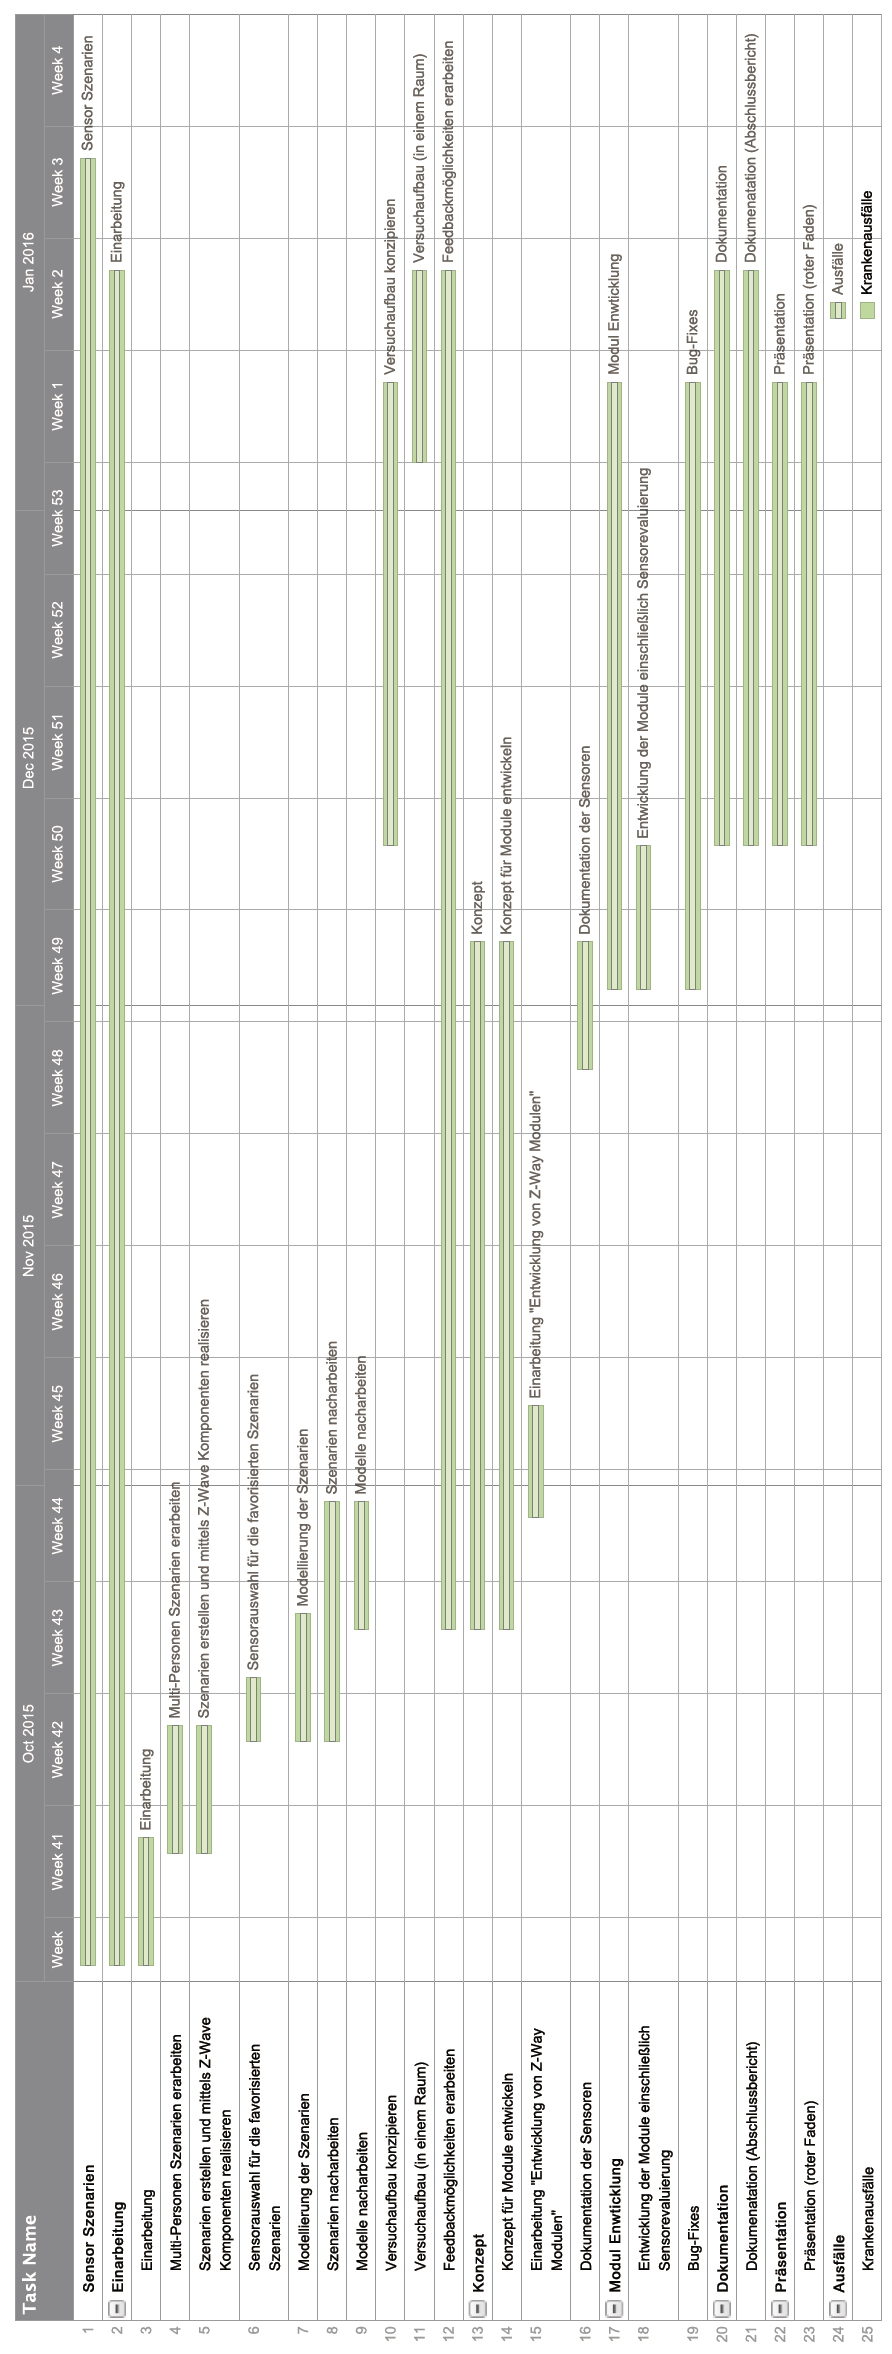
\includegraphics[width=0.55\textwidth]{img/Projektverlauf/GanttDiagramm.png}
	\caption{Gantt-Diagramm, tatsächlicher Projektverlauf}
	\label{fig:projektverlaufGanttDiagramm}
\end{figure}

\chapter{Arbeitsergebnisse}
%\begin{itemize}
%	\item Ergebnisse, welche für den weiteren Verlauf relevant sind (z.B. zu realisierende Szenarien)
%	\item weiterverfolgte Szenarien
%\end{itemize}

\section{Szenarien}

\subsection{Effizienz und Komfort - Erkennung der Anzahl der Personen in einem Raum}
\label{subsec:szenarioPersonCounter}
\emph{(von Philip Laube)}
\subsubsection{Ablauf}
Person A geht zusammen mit Person B vom Flur in das Wohnzimmer, während Person C in die Küche geht.
Die Lampen werden im Flur ausgeschaltet, im Wohnzimmer und in der Küche eingeschaltet.
Person D betritt die Wohnung und wird von den Personen A und B in der Tür zum Wohnzimmer begrüßt. Zusammen gehen sie ins Wohnzimmer.
Dabei werden zunächst die Lampen im Flur erneut eingeschaltet und nach der Begrüßung wieder ausgeschaltet.
Nach einiger Zeit ruft Person D zum Essen und es verlassen Personen A, B und C das Wohnzimmer und gehen in die Küche.
Sobald die letzte Person das Wohnzimmer verlassen hat, werden die Lampen im Wohnzimmer ausgeschaltet.

\subsubsection{Erforderliche Komponenten}
\begin{itemize}
	\item Z-Way Steuereinheit
	\item 2 x Bewegungsmelder / Fibaro 6-in-1 Sensor pro Tür
	\item Modul zur Lichtsteuerung
\end{itemize}

\subsubsection{zur Diskussion}
Es ist unbekannt, ob die Begrüßungssituation ausreichend abgegrenzt werden kann, ohne Fehler hervorzubringen.
Türen könnten zusätzlich mit Türsensoren ausgestattet werden, um ein Durchgehen zu bestätigen bzw. vorbeigehende Personen bei geschlossener Tür zu ignorieren.

\subsubsection{Modellierung Erkennung der Personenanzahl}
Das Modell (\prettyref{fig:szenarienPersonenerkennung}) zeigt den Ablauf für den Personenzähler bei einer Erkennung eines Personenübergangs mit unterschiedlichen Mitteln. Sofern ein Übergang erkannt wurde, werden die Personenzähler angepasst. Daraufhin können andere Module eine Aktion, abhängig von der nun neuen Personenanzahl pro Raum, starten.

\begin{figure}[h!]
	\centering
	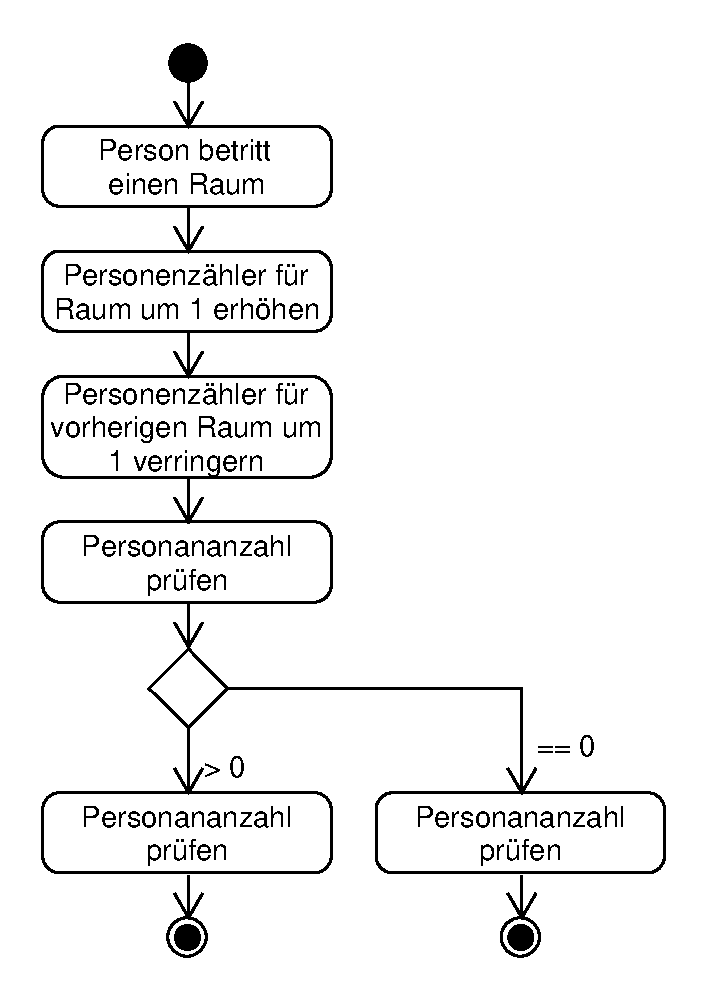
\includegraphics[scale=0.7]{img/Szenarien/ErkennungAnzahlPersonen.pdf}
	\caption{Erkennung der Personenanzahl}
	\label{fig:szenarienPersonenerkennung}
\end{figure}

\subsubsection{Modellierung Personenerkennung an der Tür}
\label{subsec:szenarioPersonTuer}
Das Modell (\prettyref{fig:szenarienPersonenerkennungTür}) zeigt den Ablauf für die beiden Bewegungssensoren an einem Türdurchgang. Dabei wird nach einer Aktivierung eines Sensors, auf einer Seite der Tür, auf den zweiten Sensor, auf der anderen Seite der Tür, eine gewisse Zeit gewartet. Sofern beide Sensoren innerhalb dieses gewissen Zeitraums aktiviert wurden, ist ein Durchgang erkannt worden und die jeweiligen Personenzähler der anliegenden Räume werden angepasst.

\begin{figure}[h!]
	\centering
	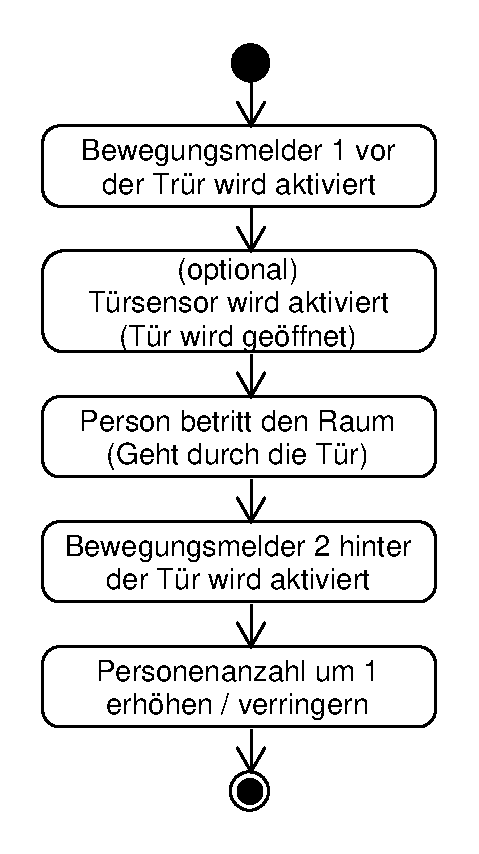
\includegraphics[scale=0.7]{img/Szenarien/PersonenerkennungAnTuer.pdf}
	\caption{Personenerkennung an der Tür}
	\label{fig:szenarienPersonenerkennungTür}
\end{figure}

\subsection{Haus bei verschließen der Haus-/ Wohnungstür in "`Standby"' versetzen}
\label{subsec:szenarioStandby}
\emph{(von Simon Schwabe)}
\subsubsection{Ablauf}
Um den Komfort in ihrem Smart Home zu steigern, möchte Anne möglichst wenig Aufwand zur Steuerung des Lichts betreiben. Dazu möchte sie bei Verlassen der Wohnung nicht alle angeschalteten Lampen manuell ausschalten und überprüfen, ob Gefahrenquellen vom Stromnetz getrennt sind.

Ein intelligentes, vernetztes Türschloss überträgt dazu beim Abschließen der Wohnung ein entsprechendes Signal an die zentrale Steuereinheit. Diese Steuereinheit interpretiert das Signal und schaltet alle Lampen aus. Außerdem werden vorher konfigurierte Steckdosen deaktiviert, um das Brandrisiko zu minimieren. Damit wird die Wohnung in einen "`Standby-Modus"' versetzt. Auch in diesem Fall möchte Anne nicht alle Geräte vom Stromnetz trennen, ihr Laptop soll weiterhin mit Strom versorgt und der Akku geladen werden.

Befindet sich Tom noch in der Wohnung, wenn sie abschließt, soll er nicht durch die Steuerung gestört werden. Das heißt in diesem Fall wird die automatische Abschaltung nicht durchgeführt. Dazu ist es notwendig, dass verschiedene Sensoren des Systems zuverlässig erkennen, ob Personen anwesend sind. Die automatische Steuerung wird erst aktiv, wenn der letzte Bewohner die Wohnung verlässt und abschließt.

Der Standby-Modus wird mit Aufschließen der Wohnungstür deaktiviert. Es erscheint allerdings nicht sinnvoll, den Zustand zum Zeitpunkt des Verlassens wiederherzustellen, da die Anforderungen an Beleuchtung usw. beim Ankommen grundlegend andere als bei Verlassen der Wohnung sein können. Diese sind abhängig von der Tageszeit.

\subsubsection{zur Diskussion}
\begin{itemize}
	\item welche Komponenten sind von der Abschaltung betroffen (z.B. Lampen, Steckdosen von Wasserkocher, Kaffeemaschine, ...)
	\item welche Komponenten sind ausgeschlossen (z.B. Kühl- und Gefrierschränke, Waschmaschinen, ...)
\end{itemize}

\subsubsection{erforderliche Komponenten}
\begin{itemize}
	\item Steuereinheit
	\item vernetztes Türschloss
	\item Sensoren zur Personenerkennung: z.B. Bewegungsmelder, Infrarot
	\item schaltbare Steckdosen, evtl. mit Verbrauchserkennung
	\item schaltbare Lampen
\end{itemize}


\subsubsection{Modellierung aus Nutzersicht}
Das Modell (\prettyref{fig:szenarienStandbyNutzersicht}) verdeutlicht die im Szenario beschriebene Interaktion des Nutzers mit dem System. Ziel des Szenarios ist es, dem Nutzer möglichst hohen Komfort zu bieten. Aus diesem Grund sind die Interaktionsmöglichkeiten des Nutzers mit dem System bewusst auf das Notwendigste beschränkt. Das Szenario wird indirekt durch den Nutzer initiiert, indem er die Wohnungstür abschließt. Auf diese Weise entsteht für die Nutzer kein Mehraufwand und keine direkte Interaktion mit dem System.

Mit dem Abschließen der Tür ist die Erwartung des Nutzers verbunden, dass die Wohnung in einen Standby-Modus tritt. Sollte dies aufgrund anwesender Personen nicht möglich sein, sollte der Nutzer über ein geeignetes Mittel darüber informiert werden. Dazu kann beispielsweise eine Benachrichtigung auf das Mobiltelefon des Nutzers gesendet werden.

\begin{figure}[h!]
	\centering
	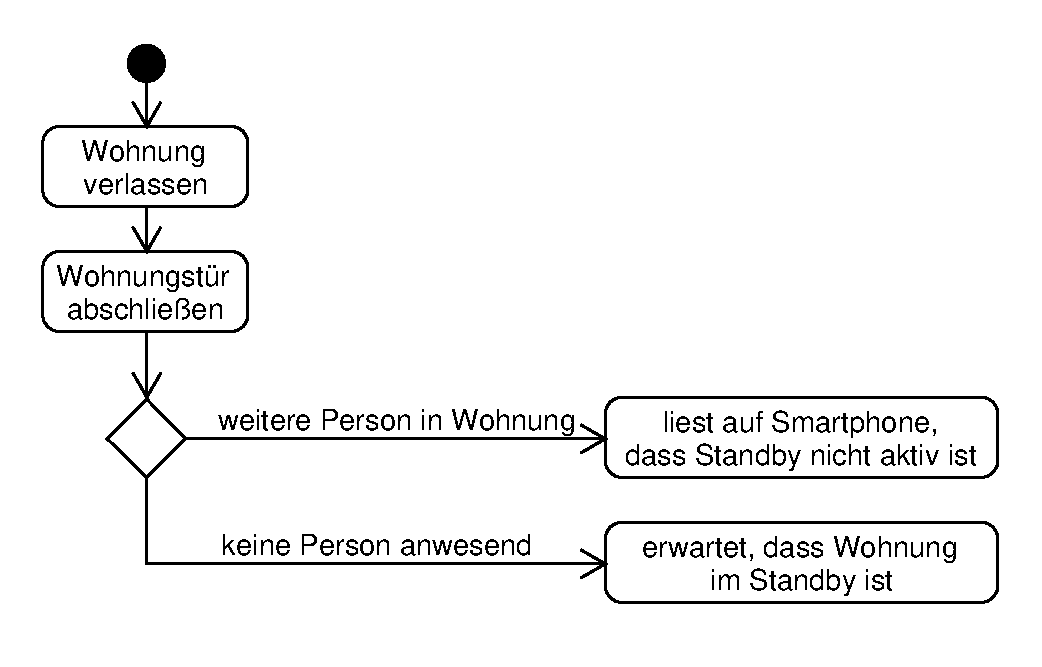
\includegraphics[scale=0.7]{img/Szenarien/WohnungSchliessenNutzersicht.pdf}
	\caption{Abläufe bei Verschließen der Wohnung aus Nutzersicht}
	\label{fig:szenarienStandbyNutzersicht}
\end{figure}

\subsubsection{Modellierung aus Systemsicht}
Die technische Modellierung (\prettyref{fig:szenarienStandby}) gestaltet sich etwas umfangreicher. Gestartet wird der Ablauf durch das Schließen des konfigurierten Schlosses. Alternativ kann auch ein Schalter an der Wohnungstür betätigt werden. Das System überprüft daraufhin, ob noch Personen in der Wohnung anwesend sind. Ist das der Fall, wird die Aktion abgebrochen und anwesende Personen werden nicht in ihren Aktivitäten beeinträchtigt. In diesem Fall kann der Nutzer, welcher die Wohnung verlassen hat, informiert werden.

Wird zum Zeitpunkt des Abschließens keine anwesende Person erkannt, wird ein Timer gestartet. So lange dieser Timer aktiv ist, wird in regelmäßigen Abständen überprüft, ob Personen, bzw. Bewegungen in der Wohnung erkannt werden. Dieses Vorgehen soll die Gefahr reduzieren, dass anwesende Personen nicht wahrgenommen werden. Wird während der Laufzeit des Timers eine Person erkannt, wird die Aktion wie oben beschrieben abgebrochen.

Trotz dieses Vorgehens ist nicht auszuschließen, dass Personen in der Wohnung nicht korrekt erkannt werden. Für diesen Fall kann ein zusätzlicher Feedback-Modus implementiert werden, in dem die anwesenden, nicht erkannten Personen über die anstehende Aktion informiert werden. Erfolgt kein Feedback, werden konfigurierte Geräte in den Standby-Modus versetzt.

\begin{figure}[h!]
	\centering
	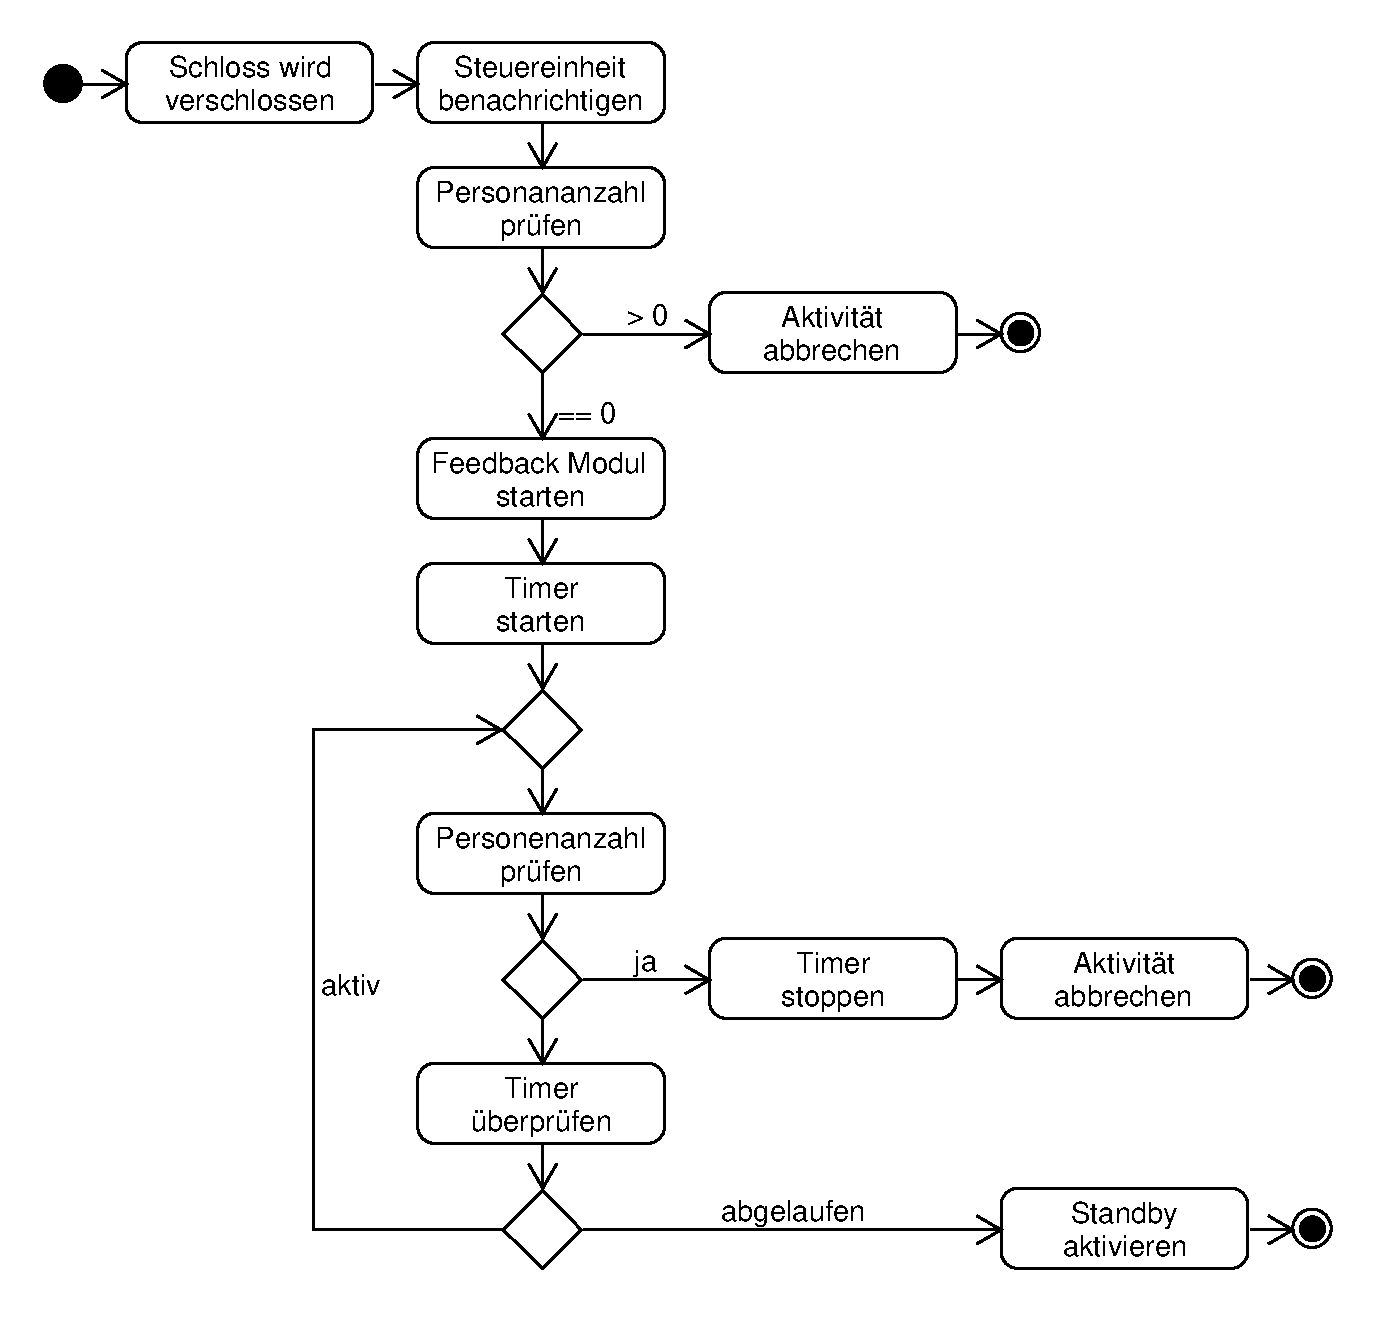
\includegraphics[width=0.9\textwidth]{img/Szenarien/WohnungSchliessen.pdf}
	\caption{Abläufe bei Verschließen der Wohnung aus Systemsicht}
	\label{fig:szenarienStandby}
\end{figure}

\subsection{Gefahrenquellen abstellen (Fibaro, CO$_2$)}
\label{subsec:szenarioGefahrenquellen}
\emph{(von Martin Petzold)}
\subsubsection{Auslöser (opt.)}
\begin{itemize}
	\item Erkennung Erwachsene Person (Fibaro, CO$_2$)
\end{itemize}

\subsubsection{Vorbedingung}
\begin{itemize}
	\item Zuverlässige Erkennung ob Personen den Raum betreten oder verlassen (\prettyref{subsec:szenarioPersonTuer})
\end{itemize}

\subsubsection{Ablauf}
Das System befindet sich im Standby, d.h. alle Gefahrenquellen im Raum sind ausgeschaltet. Person X (ein Kind) betritt den Raum. Das Betreten des Raumes wird vom System erkannt und es wird ein Vorgang gestartet, der die Person als Kind oder Erwachsenen identifiziert. Person X wird dabei als Kind identifiziert und die Gefahrenquellen bleiben somit abgeschaltet. 
Nun betritt Person Y (ein Erwachsener) den Raum, dessen Betreten wird ebenfalls vom System erkannt. Der Erkennungsvorgang wird ein zweites Mal gestartet. Das System erkennt, dass es sich bei einer der beiden Personen um eine erwachsene Person handelt und schaltet die Gefahrenquellen frei, so dass diese benutzt werden können.
Nach einer Weile verlässt Person Y den Raum. Das System stellt fest das sich kein Erwachsener mehr im Raum befindet und schaltet nach einer gewissen Zeit den Standby Modus wieder her.

\subsubsection{Alternativer Ablauf}
Nur Person Y (ein Erwachsener) betritt den Raum und das System erkennt den Eintritt. Er wird beim Identifizierungsvorgang als Erwachsener erkannt und damit werden die Gefahrenquellen freigeschaltet.
Nach einer Weile verlässt Person Y den Raum. Das System stellt fest das sich kein Erwachsener mehr im Raum befindet und schaltet nach einer gewissen Zeit den Standby Modus wieder her.

\subsubsection{erforderliche Komponenten}
\begin{itemize}
	\item Fibaro 6 in 1 Sensor
	\item CO$_2$ Sensor
	\item Z-Way-Server/Steuereinheit
	\item 2 Bewegungsmelder zur Erkennung von Eintritt in den Raum
	\item Schaltbare Gefahrenquelle oder zur Simulation eine schaltbare Lampe
\end{itemize}

\subsubsection{Nachbedingung}
\begin{itemize}
	\item Das System kann auch eine Regelung beinhalten, dass der Standby Modus automatisch und nicht nach verlassen des Raumes zeitgesteuert wieder hergestellt wird.
\end{itemize}

\subsubsection{zur Diskussion}
\begin{itemize}
	\item Abgleich mit dem Szenario zur Erkennung ob eine Person den Raum betreten/verlassen hat
	\item sind die Sensoren präzise genug um den Unterschied zwischen Kind und Erwachsener zu erfassen, oder kann nur Mensch und Haustier unterschieden werden
	\item soll die Reaktivierung des Standby Modus Teil des Szenarios sein
	\item Einordnung in umsetzbar/nicht umsetzbar
\end{itemize}

\subsubsection{ähnliche Szenarien}
\begin{itemize}
	\item \prettyref{subsec:szenarioPersonTuer}
	\item \prettyref{subsec:szenarioStandby}
\end{itemize}

\subsubsection{Modellierung Identifizierung Erwachsener}
\emph(//TODO BITTE NOCH BESCHREIBUNGSTEXT EINFÜGEN (siehe Modell)) bereits gemacht?

Wenn sich die Personenanzahl eines Raumes ändert wird unterschieden, ob die Person den Raum betreten oder verlassen hat. Danach wird die Größenmessung und CO$_2$ Messung gestartet. Wenn eine Person den Raum betreten hat, wird die Größenerkennung abgeglichen und anhand des Ergebnisses die Anzahl der Erwachsenen erhöht. Verlässt eine Person den Raum, dann wird der Counter verringert. Wenn der erwachsenenCounter Geringer als 1 ist oder die CO$_2$ Messung keinen Erwachsenen erkennt wird der Vorgang mit kein Erwachsener vorhanden beendet. Nur wenn sowohl die Größenmessung und die CO$_2$ Messung einen Erwachsenen erkennen, wird "`Erwachsener erkannt"' ausgegeben.
\begin{figure}[h!]
	\centering
	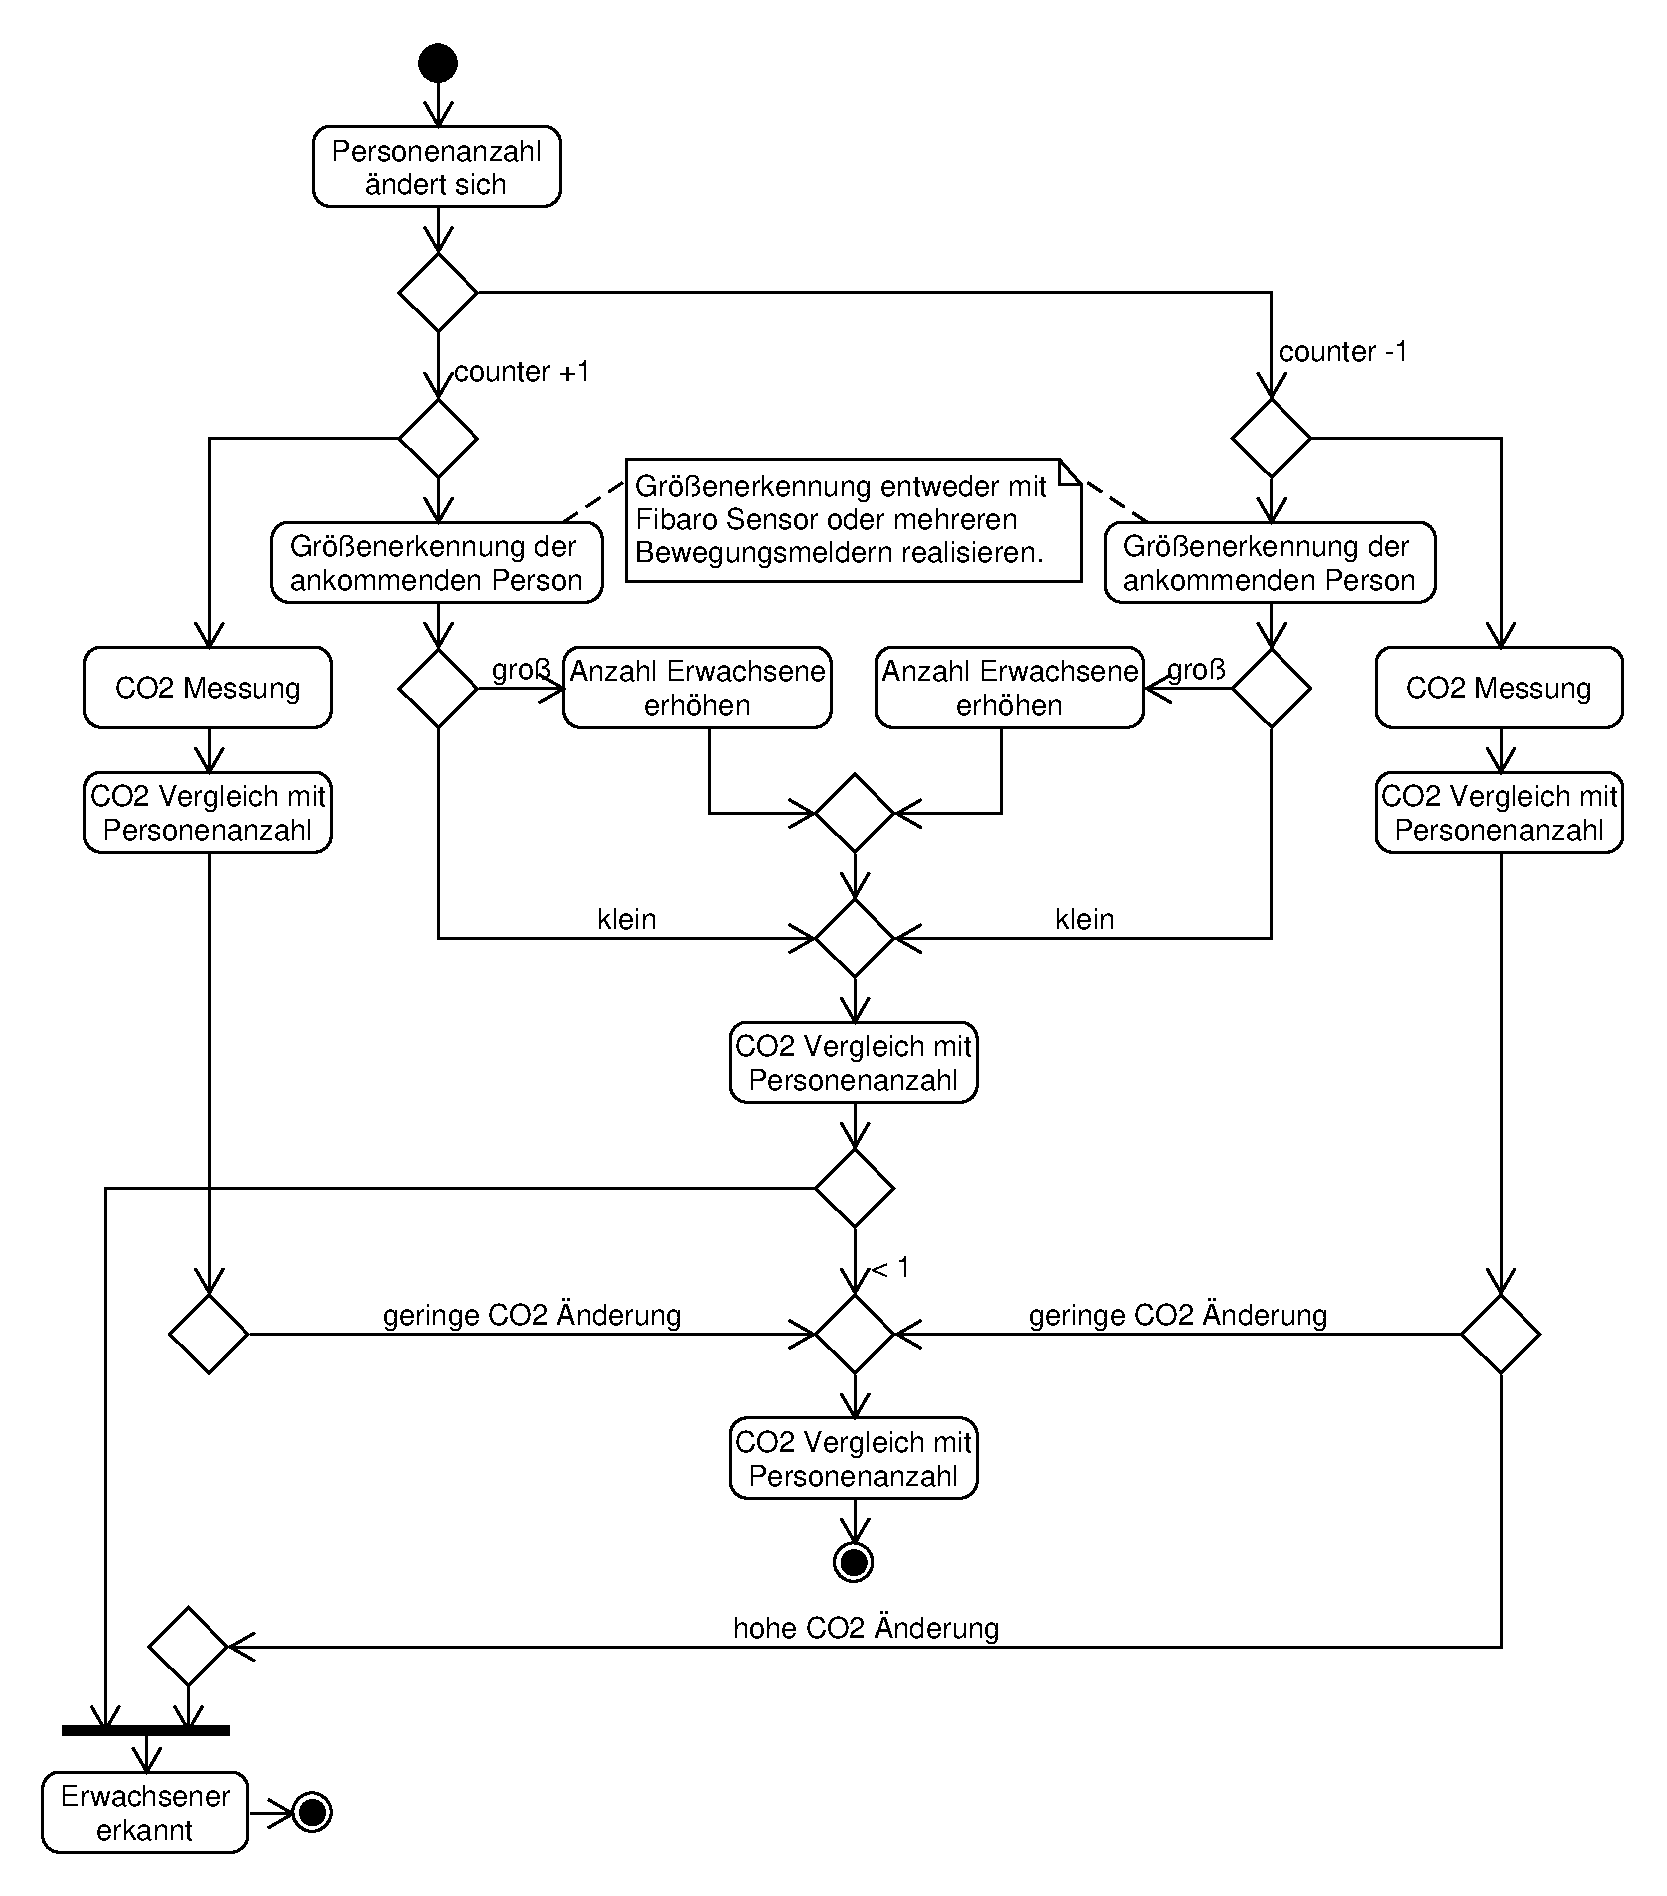
\includegraphics[width=0.9\textwidth]{img/Szenarien/IdentifizierungErwachsene.pdf}
	\caption{Identifizierung Erwachsener}
	\label{fig:szenarienIdentifizierungErwachsene}
\end{figure}

\subsubsection{Modellierung Gefahrenquellen abstellen}
\emph(//TODO BITTE NOCH BESCHREIBUNGSTEXT EINFÜGEN (siehe Modell)) bereits gemacht?

Wenn sich die Personenanzahl eines PersonCounters ändert, wird die Identifizierung gestartet, ob sich ein Erwachsener im Raum befindet. Wird ein Erwachsener erkannt wird der Zustand der Gefahrenquellen ausgelesen und, wenn nötig, freigeschaltet. Wird bei der Identifizierung kein Erwachsener erkannt wird ebenfalls der Zustand der Gefahrenquellen ausgelesen und gegebenenfalls ein Timer zu deren Abschaltung gestartet, welcher bei erneuter Änderung der Personenanzahl gestoppt wird.

\begin{figure}[h!]
	\centering
	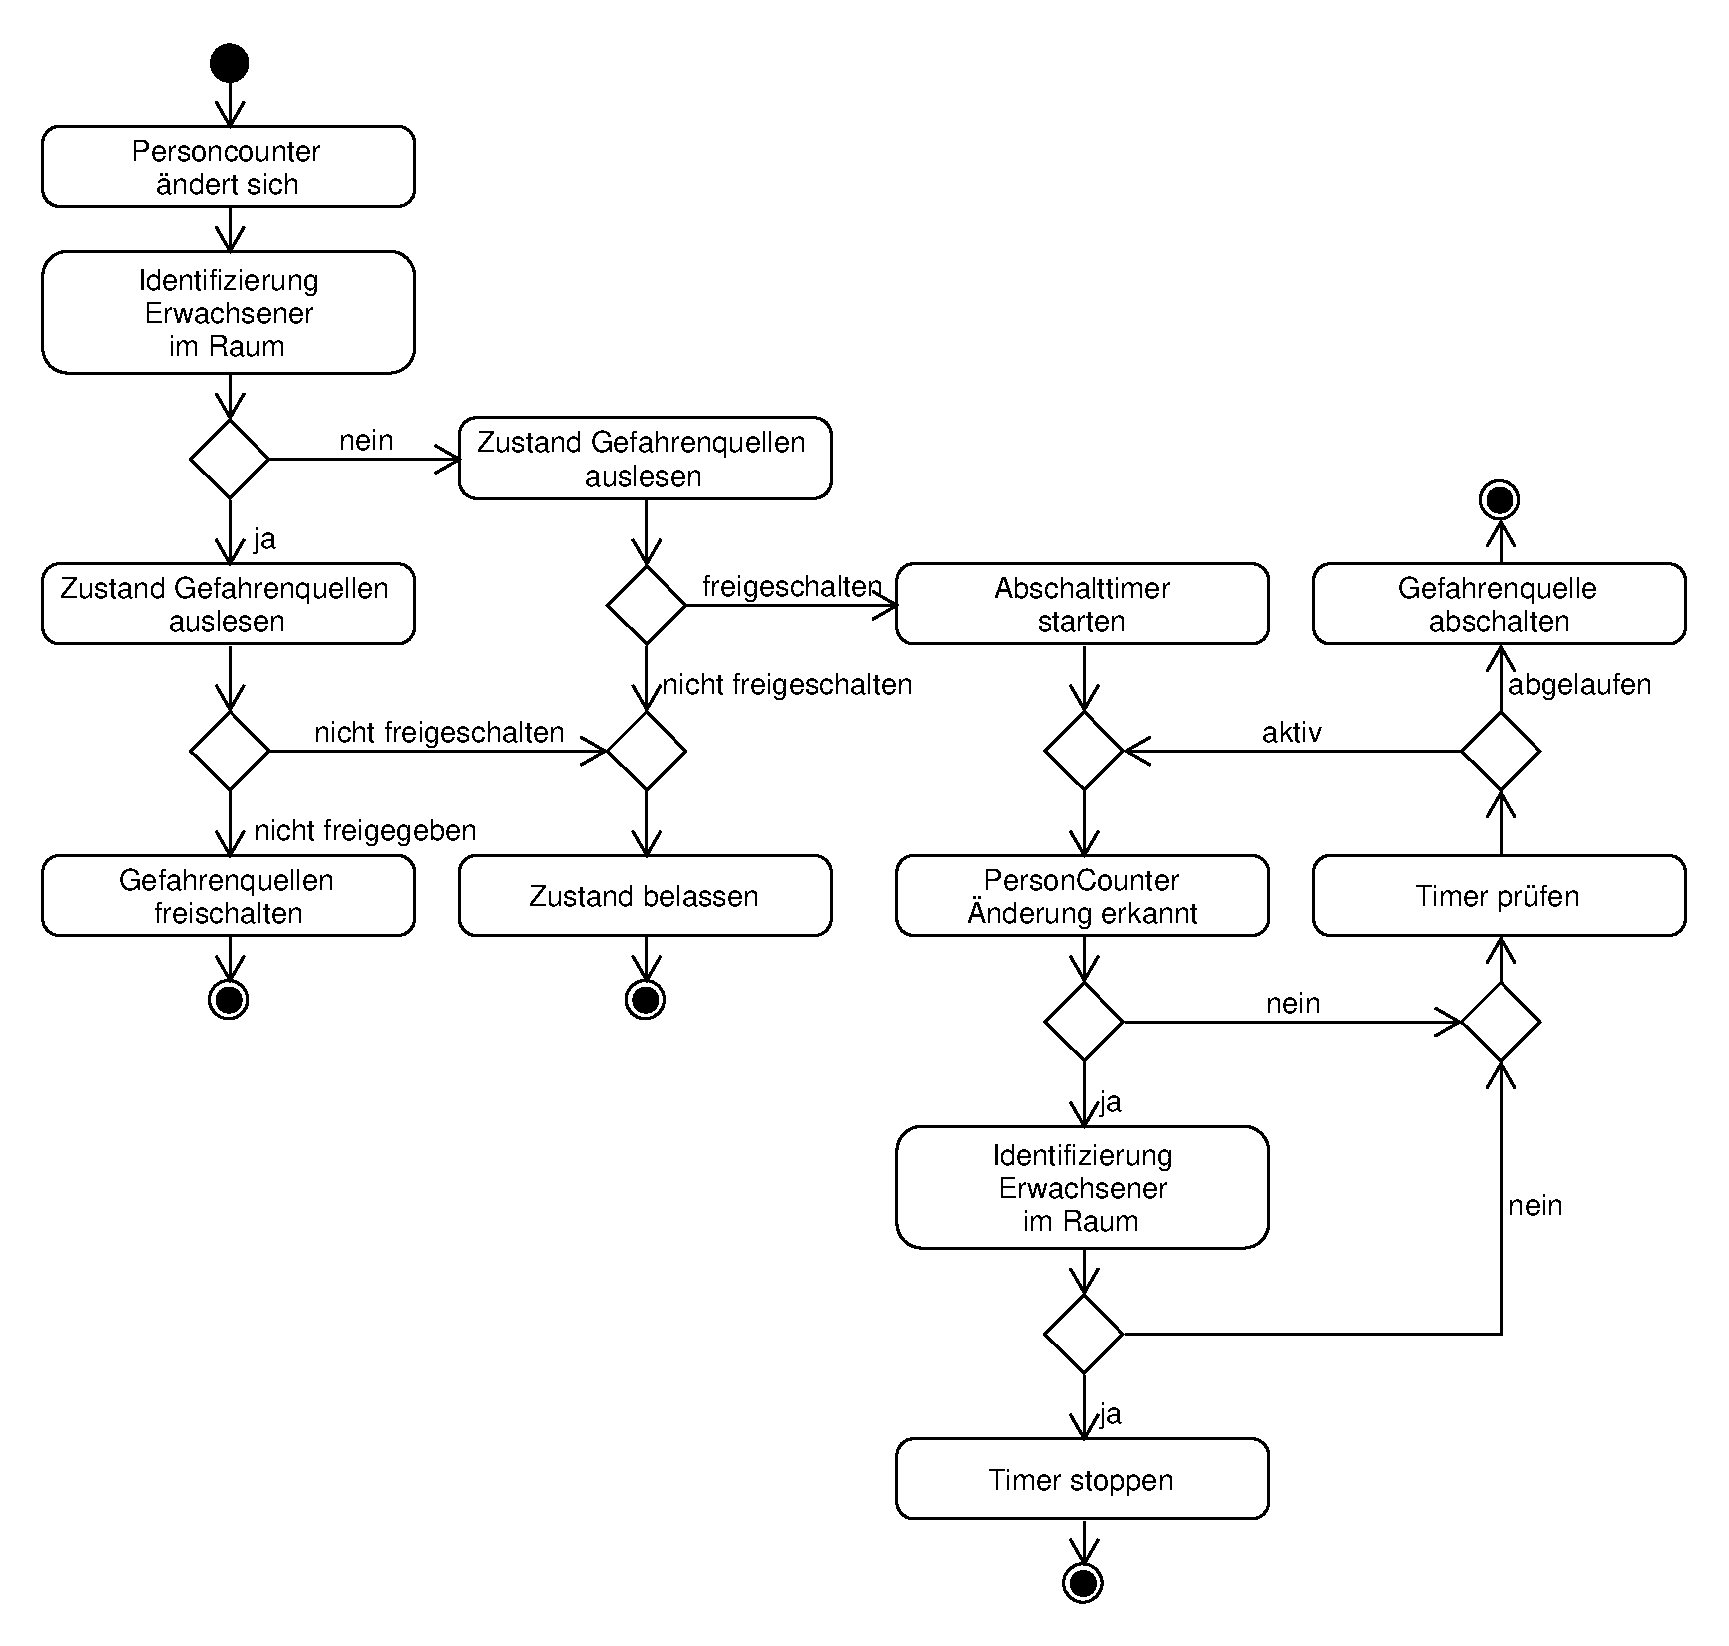
\includegraphics[width=0.9\textwidth]{img/Szenarien/GefahrenquellenAbstellen.pdf}
	\caption{Gefahrenquellen abstellen}
	\label{fig:szenarienGefahrenquellenAbstellen}
\end{figure}


\section{Modulkonzeption}
\label{sec:modulkonzepte}
TODO: allgemeine Beschreibung aller Module, deren Zusammenwirken (Grafik).

\subsection{LockDoorModule}
\emph{(von Simon Schwabe)}

\subsubsection{Allgemein}
Das \emph{LockDoorModule} ist der Vermittler für weitere Module im Zusammenhang mit dem Verlassen der Wohnung. Wenn die Wohnung verlassen und abgeschlossen wird, ist die Wahrscheinlichkeit hoch, dass keine weiteren Personen anwesend sind. Allerdings kann die Wohnung auch irrtümlich abgeschlossen werden und es sind noch weitere Personen anwesend. Um solchen Fehlinterpretationen entgegenzuwirken überprüft das \emph{LockDoorModule} immer, ob wirklich keine Personen erkannt werden und die Wohnung leer steht. Diese Information ist für weitere Module, insbesondere das \emph{AlarmModule}, relevant und wird über den Event Bus mitgeteilt.

\subsubsection{Funktionsweise}
Die genaue Funktionsweise des Moduls wurde im Wesentlichen schon im Abschnitt Szenarien (siehe \prettyref{subsec:szenarioStandby}) beschrieben und modelliert. Das Modell "`Abläufe bei Verschließen der Wohnung aus Systemsicht"' (\prettyref{fig:szenarienStandby}) beschreibt das Vorgehen. Die Aktivität „Standby aktivieren“ kann um das Werfen des entsprechenden Events erweitert werden.

Das Szenario enthält keine detaillierte Beschreibung für die Abschaltung des Standby-Modus, da dies nicht notwendig ist. Für das \emph{LockDoorModule} ist es allerdings erforderlich auf die Ankunft von Personen zu reagieren, z.B. um das \emph{AlarmModule} zu benachrichtigen und die Alarmanlage abzuschalten. %Die Anzahl der durchzuführenden Aktionen ist überschaubar und wird im Modell dargestellt (\prettyref{fig:modulkonzeptionLockDoorSequence}).
Dazu wird bei Ankunft der entsprechende Schalter betätigt, bzw. das Schloss geschlossen. Anschließend wird das Event \emph{LockDoorModule\_unlocked} geworfen. An dieser Stelle ist keine weitere Logik erforderlich.

Das Sequenzdiagramm (\prettyref{fig:modulkonzeptionLockDoorSequence}) stellt mögliche Abläufe bei dem Verschließen der Tür dar. Im ersten Fall ist die Personenanzahl des abgefragten \emph{PersonCounters} sieben, es sind demzufolge noch Personen anwesend und es werden keine weiteren Aktionen durchgeführt. Im zweiten Ablauf erkennt der \emph{PersonCounter} keine anwesenden Personen. Da dies auch eine Fehleinschätzung sein kann, wird in diesem Fall das \emph{InHomeFeedbackModule} aktiviert und über einen Aufruf der ZAutomation-API der Feedback-Modus gestartet. Dieser ermöglicht es eventuell anwesenden Personen auf die anstehende Aktion zu reagieren.

\begin{figure}[h!]
	\centering
	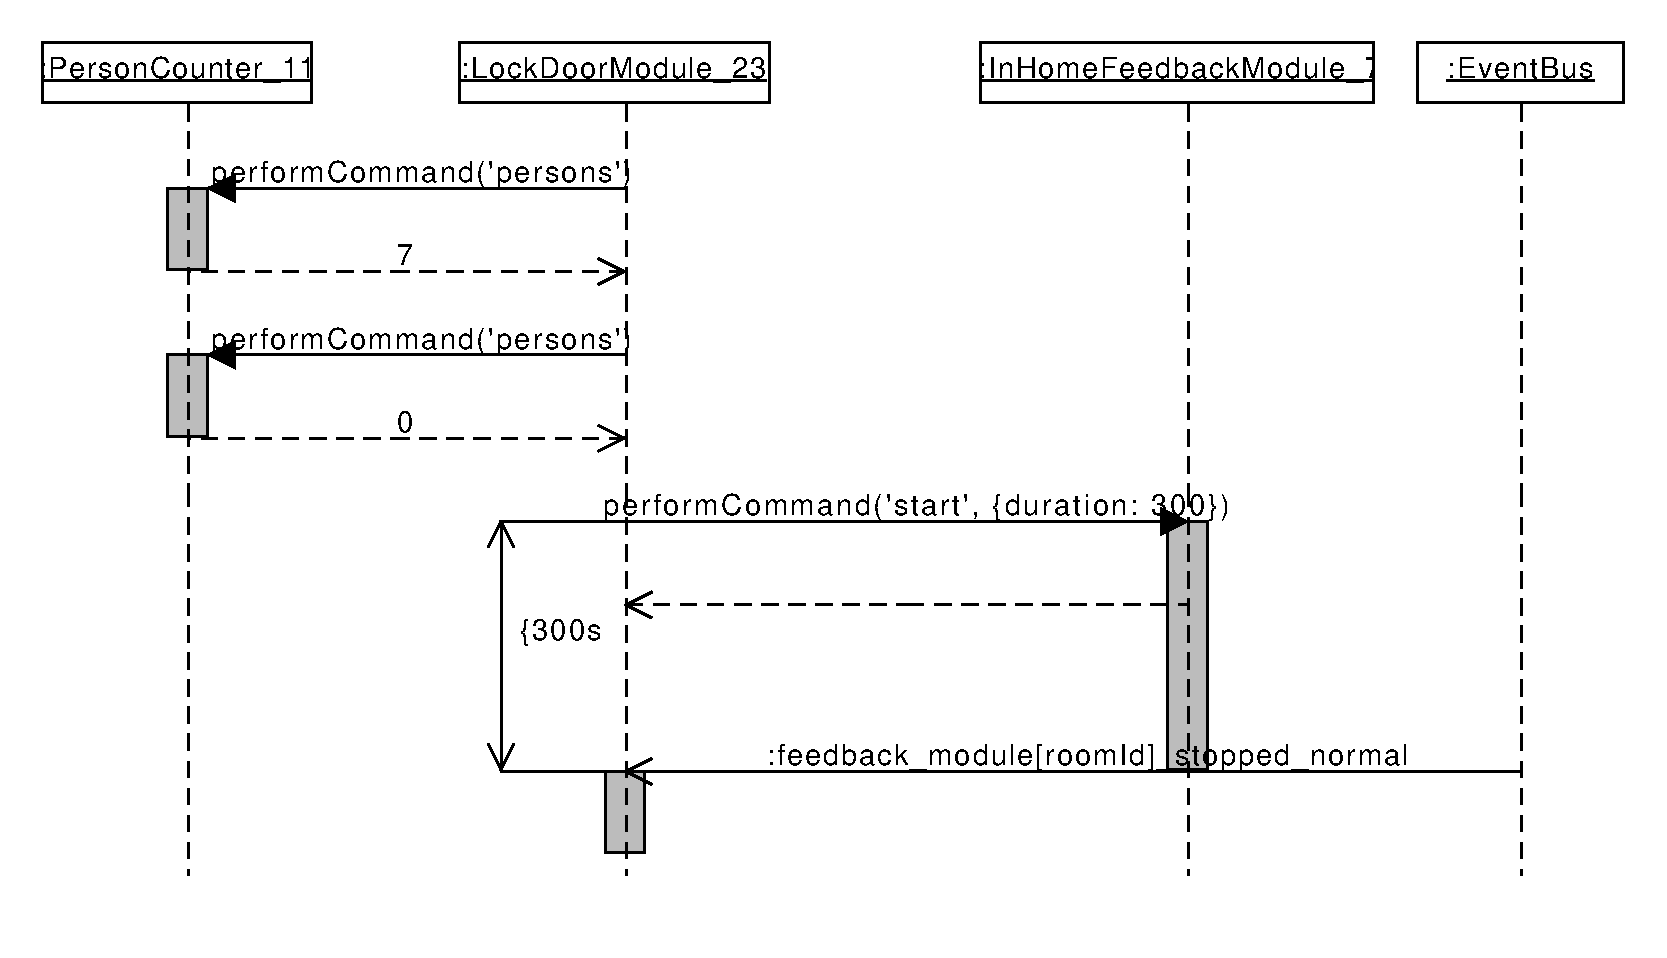
\includegraphics[width=0.9\textwidth]{img/Modulkonzeption/LockDoorSequence.pdf}
	\caption{\emph{LockDoorModule:} Sequenzdiagramm}
	\label{fig:modulkonzeptionLockDoorSequence}
\end{figure}

\subsubsection{Konfiguration}
Bei der Konfiguration des \emph{LockDoorModule} muss das Wohnungstürschloss angegeben werden, alternativ kann dafür ein Schalter benutzt werden, der im Inneren der Wohnung vor dem Verlassen betätigt wird. 
\begin{itemize}
	\item Schloss/Schalter
	\begin{itemize}
		\item Typ: BinarySwitch
		\item erforderlich: ja
	\end{itemize}
\end{itemize}

\subsubsection{Schnittstellen}
Die Schnittstellen, welche dieses Modul nutzt und bereitstellt, sind von großer Bedeutung. Das Modul an sich implementiert eine nur geringe Funktionalität, jedoch ist es eine Brücke zwischen den Modulen zur Raumüberwachung auf der einen Seite, und den Modulen für Aktionen beim Verlassen der Wohnung auf der anderen Seite.

Das \emph{LockDoorModule} bietet über den Event Bus eine Schnittstelle zu anderen Modulen. Diese werden benachrichtigt, sobald davon ausgegangen wird, dass keine Person mehr anwesend ist (\emph{LockDoorModule\_locked}). Die Freischaltung geschieht über ein weiteres Event (\emph{LockDoorModule\_unlocked}).

Das Modul wird als Singleton angelegt, da für jede Wohnung nur ein Modul zur Überwachung der Wohnungstür erforderlich ist. Das hat zur Folge, dass Events keine \emph{VirtualDeviceId} tragen. Damit ist es für Empfänger einfacher, auf entsprechende Events zu reagieren.

Für die Überprüfung der Personenanzahl wird die Schnittstelle \emph{PersonCounterModule} genutzt. Dazu wird für jeden Raum die Anzahl der Personen überprüft.

\begin{table}[h!]
\begin{tabularx}{\textwidth}{
		 >{\hsize=1.25\hsize}X % 40% of 3\hsize 
		>{\hsize=0.5\hsize\centering}X % 30% of 3\hsize
		>{\hsize=1.25\hsize}X % 40% of 3\hsize
		% sum=3.0\hsize for 3 columns
	}
	\hline
	\textbf{Event Name}					& \textbf{Parameter}	& \textbf{Beschreibung} \\
	\hline LockDoorModule\_locked		& - 					& Tür verschlossen, keine Person anwesend \\ 
	\hline LockDoorModule\_unlocked		& - 			 		& Tür geöffnet \\ 
	\hline
\end{tabularx}
\caption{LockDoorModule: Schnittstelle Event Bus}
\end{table}


\subsubsection{Abhängigkeiten}
\begin{itemize}
	\item \emph{PersonCounterModule}
	\item \emph{TurnOffTimerModule}
\end{itemize}
Das \emph{PersonCounterModule} wird zur Überprüfung der Personenanzahl je Raum genutzt. Dazu werden Aufrufe über die ZAutomation-API an das Modul gesendet.

Das \emph{TurnOffTimerModule} stellt eine Schnittstelle zum \emph{FeedbackModule} her. Durch die zusätzliche Abstraktionsschicht des \emph{TurnOffTimerModule} arbeitet das \emph{LockDoorModule} nicht direkt gegen das \emph{FeedbackModule}, sondern startet lediglich den \emph{TurnOffTimer}. Dieser übernimmt die Kommunikation mit dem \emph{FeedbackModule}.

\subsubsection{Interne Speicher}
\begin{itemize}
	\item konfiguriertes Türschloss
\end{itemize}


\subsection{PersonCounterModule}
\emph{(von Philip Laube)}
\subsubsection{Allgemein}
Das \emph{PersonCounterModule} übernimmt die Aufgabe, die Anzahl der Personen im jeweiligen Raum zu speichern. Jede Möglichkeit einer Erkennung ob eine Person den Raum betreten oder verlassen hat kann über dieses Modul kommuniziert werden um es anderen Modulen zur Verfügung zu stellen. Dies macht dieses Modul zu einem zentralen Bestandteil.

Ein \emph{PersonCounterModule} enthält zusätzlich die Information, für welchen Raum es bestimmt ist. Somit kann es beliebig oft wiederverwendet werden.

Der jeweilige Personenzähler pro Raum wird durch Module, die ihn benötigen, instanziiert. Vorhandene Personenzähler werden einfach verwendet.

\subsubsection{Funktionsweise}
Dieses Modul wird nur indirekt benutzt. Es dient als Datenhaltung für die wichtige und von anderen Modulen benötige Informationen der Personenanzahl (\prettyref{fig:szenarienPersonenerkennung}).

Die Instanziierung des Moduls findet entweder zentral über ein Modul statt oder wird als Funktion bereitgestellt. Es kann dann entweder automatisch oder pro Modul über eine Funktion instanziiert und benutzt werden.

\subsubsection{Konfiguration}
\begin{itemize}
	\item Zähler
	\begin{itemize}
		\item Typ: Metrik
		\item erforderlich: ja
	\end{itemize}
	\item Raum
	\begin{itemize}
		\item Typ: Text
		\item erforderlich: ja
	\end{itemize}
\end{itemize}

\subsubsection{Schnittstellen}

\begin{table}[H]
	\begin{tabularx}{\textwidth}{
			>{\hsize=1.25\hsize}X % 40% of 3\hsize 
			>{\hsize=0.5\hsize\centering}X % 30% of 3\hsize
			>{\hsize=1.25\hsize}X % 40% of 3\hsize
			% sum=3.0\hsize for 3 columns
		}
		\hline
		\textbf{URL}						& \textbf{Parameter}	& \textbf{Beschreibung} \\
		\hline /command/person\_entered		& - 					& Erhöht den Zähler um 1. \\ 
		\hline /command/person\_left		& - 			 		& Mindert den Zähler um 1. \\
		\hline /command/persons				& - 					& Liefert die aktuelle Anzahl an Personen des Raums. \\
		\hline
	\end{tabularx}
	\caption{\emph{PersonCounterModule}: Schnittstelle ZAutomation}
\end{table}

\begin{table}[H]
	\begin{tabularx}{\textwidth}{
			>{\hsize=1.5\hsize}X 
			>{\hsize=0.5\hsize}X
		}
		\hline
		\textbf{Event Name}													& \textbf{Beschreibung} \\
		\hline [DeviceId]:PersonCounterModule\_[RaumId]\_person\_entered	& - \\ 
		\hline [DeviceId]:PersonCounterModule\_[RaumId]\_person\_left		& - \\
		\hline
	\end{tabularx}
	\caption{\emph{PersonCounterModule}: Schnittstelle Event Bus}
\end{table}

\subsubsection{Abhängigkeiten}
\begin{itemize}
	\item Keine, da dieses Modul Grundfunktionalitäten bereitstellt.
\end{itemize}

\subsubsection{Interne Speicher}
\begin{itemize}
	\item Raum ID
	\item Anzahl der Personen im Raum
\end{itemize}


\subsection{RoomAccessModule}
\emph{(von Philip Laube)}

\subsubsection{Allgemein}
Das \emph{RoomAccessModule} übernimmt die Aufgabe, Personen zu erkennen, die einen Raum verlassen oder betreten haben. Dies geschieht entweder unverzüglich oder zeitversetzt, je nach Art der zugrundeliegende Module.

Dieses Modul stellt grundlegende Unterstützung zunächst für Bewegungssensoren, später eventuell auch erweiterte Logik für andere Sensoren zur Personenerkennung bzw. Raumwechsel.

Ein \emph{RoomAccessModule} enthält zusätzlich die Information für welche Räume es bestimmt ist, somit kann es beliebig oft wiederverwendet werden.

\subsubsection{Funktionsweise}
Diese Realisierung entspricht der geplanten Realisierung des Szenarios zu Beginn des Projekts (\prettyref{subsec:szenarioPersonCounter}). Exakt diese Logik wird zunächst durch dieses Modul implementiert (\prettyref{fig:szenarienPersonenerkennungTür}).

Es wird der zugehörige Personenzähler der jeweiligen Räume angesprochen und die Anzahl jeweils korrigiert. Weitere Logik anderer Module kann durch ein Event erfolgen. Jedwede Logik die direkt mit der Personenanzahl in Verbindung steht muss den Personenzähler (\emph{PersonCounterModule}) ansprechen.

\subsubsection{Konfiguration}
\begin{itemize}
	\item Sensor Eins
	\begin{itemize}
		\item Typ: Bewegungssensor
		\item erforderlich: ja
	\end{itemize}
	
	\item Raum Eins
	\begin{itemize}
		\item Typ: Raum
		\item erforderlich: ja
	\end{itemize}

	\item Sensor Zwei
	\begin{itemize}
		\item Typ: Bewegungssensor
		\item erforderlich: ja
	\end{itemize}
	
	\item Raum Zwei
	\begin{itemize}
		\item Typ: Raum
		\item erforderlich: ja
	\end{itemize}
\end{itemize}

\subsubsection{Schnittstellen}
\begin{table}[H]
	\begin{tabularx}{\textwidth}{
			>{\hsize=1.25\hsize}X 
			>{\hsize=0.75\hsize}X
			% sum=2.0\hsize for 2 columns
		}
		\hline
		\textbf{Event Name}						& \textbf{Beschreibung} \\
		\hline [DeviceId]:RoomAccessModule\_[verlassenderRaumId]\_[betretenerRaumId]\_transition\_detected	& Wenn ein Übergang einer Person von einem Raum in den nächsten 	Raum erfolgt ist wird dieses Event ausgelöst \\ 
		\hline 
	\end{tabularx}
	\caption{\emph{RoomAccessModule}: Schnittstellen Event Bus}
\end{table}

\subsubsection{Abhängigkeiten}
\begin{itemize}
	\item Daten des \emph{PersonCounterModule} zum Zählen der Personen in einem Raum
\end{itemize}

\subsubsection{Interne Speicher}
\begin{itemize}
	\item zwei Bewegungssensoren
	\item Raum Zuordnung der beiden Sensoren
	\item \emph{PersonCounterModule} der Raumzuordnungen
\end{itemize}


\subsection{StandbyModule}
\emph{(von Zarina Muratbekovna Omurova)}
\subsubsection{Allgemein}
Das \emph{StandbyModule} übernimmt die Aufgabe, das Haus in einen Standby-Modus zu versetzen.

Im Fall, dass niemand zu Hause ist und das Event "`LockDoor\_locked"' vom \emph{LockDoorModule} eingegangen ist, werden ausgewählte Geräte, wie Lampen, Heizung oder Elektrogeräte im Haus in einen definierten Zustand geschaltet. Manche Geräte, z.B. Steckdosen, sollen ausgeschaltet werden, wenn die Wohnung in den Standby-Modus geht. Andere Geräte, z.B. Orientierungsleuchten oder Alarmanlagen sollen angeschaltet werden. Diese Geräte und die entsprechenden Aktionen werden beim Anlegen des \emph{StandbyModules} konfiguriert.

Bei dem Event "`LockDoor\_unlocked"', werden keine Aktionen durchgeführt, dies bewirkt, dass der interne Zustand des \emph{StandbyModules} auf "`stopped"' geändert wird.

Wenn die Tür geöffnet wird, wird automatisch der Standby-Modus ausgeschaltet und ein entsprechendes Event an andere Module gesendet.

\subsubsection{Funktionsweise}

\begin{figure}[h!]
	\centering
	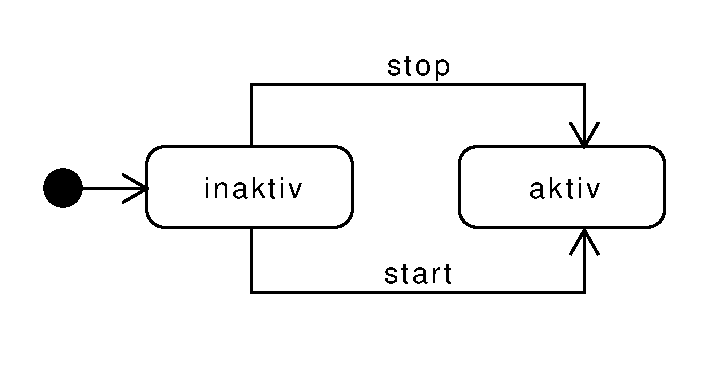
\includegraphics[scale=0.7]{img/Modulkonzeption/StandbyStateMachine.pdf}
	\caption{Zustandsdiagramm – \emph{StandbyModule}}
	\label{fig:standbyStateMachine}
\end{figure}


Dieses Modell veranschaulicht die verschiedenen internen Zustände des \emph{StandbyModules} und deren Zustandsübergänge. Wenn es im inaktiven Zustand ist, wird das Modul durch einen Startkommando in einen aktiven Zustand übergehen und im aktivem Zustand kann das Modul in einen inaktiven Zustand wechseln.

\subsubsection{Konfiguration}
\begin{itemize}
	\item Geräte, welche bei Aktivierung des Standby geschaltet werden
	\begin{itemize}
		\item 	Typ: Liste [Switch Binary, Switch Multilevel]
		\item Aktion: on/off 
		\item erforderlich: ja
	\end{itemize}
	\item Geräte, welche bei Dektivierung des Standby geschaltet werden
	\begin{itemize}
		\item 	Typ: Liste [Switch Binary, Switch Multilevel]
		\item Aktion: on/off 
		\item erforderlich: ja
	\end{itemize}
	\item Raum
	\begin{itemize}
		\item Typ: Text
		\item erforderlich: ja
	\end{itemize}
\end{itemize}

\subsubsection{Schnittstellen}
\begin{table}[H]
	\begin{tabularx}{\textwidth}{
			>{\hsize=1.25\hsize}X % 40% of 3\hsize 
			>{\hsize=0.5\hsize\centering}X % 30% of 3\hsize
			>{\hsize=1.25\hsize}X % 40% of 3\hsize
			% sum=3.0\hsize for 3 columns
		}
		\hline
		\textbf{URL}						& \textbf{Parameter}	& \textbf{Beschreibung} \\
		\hline /command/started				& - 					& Starten des Standby-Modus. \\ 
		\hline /command/stopped				& - 			 		& Stoppen des Standby-Modus. \\
		\hline /command/state				& stopped started	& Liefert den aktuellen Zustand des Moduls. \\
		\hline
	\end{tabularx}
	\caption{\emph{StandbyModule}: Schnittstelle ZAutomation}
\end{table}

\begin{table}[H]
	\begin{tabularx}{\textwidth}{
			>{\hsize=1.25\hsize}X % 66.66% of 3\hsize 
			>{\hsize=0.5\hsize\centering}X % 16.66% of 3\hsize
			>{\hsize=1.25\hsize}X % 16.66% of 3\hsize
			% sum=3.0\hsize for 3 columns
		}
		\hline
		\textbf{Event Name}								& \textbf{Parameter}	& \textbf{Beschreibung} \\
		\hline [DeviceId]:StandbyModule\_[RaumId]\_started	& - 				& Standby-Modus wurde gestartet \\ 
		\hline [DeviceId]:StandbyModule\_[RaumId]\_stopped	& - 				& Standby-Modus wurde beendet \\
		\hline
	\end{tabularx}
	\caption{\emph{StandbyModule}: Schnittstelle Event Bus}
\end{table}

\subsubsection{Abhängigkeiten}
\begin{itemize}
	\item Module Events (LockDoor)
\end{itemize}

\subsubsection{Interne Speicher}
\begin{itemize}
	\item Raum ID
	\item Zustand des Raums (im Standby: stopped/started)
	\item Switches/Dimmers
\end{itemize}


\subsection{InHomeFeedbackModule}
\emph{(von Patrick Hecker)}
\subsubsection{Allgemein}
Das \emph{FeedbackModule} übernimmt die Aufgabe, Personen im Haus über eingehende Aktionen zu informieren. Neben den eingehenden Aktionen (von Personen außerhalb des Hauses) kann auch auf Aktionen, die vom System automatisch gestartet wurden, hingewiesen werden (Timer, Grenzwert eines Sensors überschritten, ...). Die Personen im Haus haben dadurch die Möglichkeit auf Aktionen zu reagieren, indem sie sie abbrechen bzw. verzögern können. Der konkrete Feedbackmechanismus kann individuell konfiguriert werden und gliedert sich in folgende fünf Kategorien (detaillierter in Abschnitt Konfiguration).

\begin{itemize}
	\item visuelles Feedback (bspw. Lampen, LED’s an Schalter, ...),
	\item akustisches Feedback (bspw. Sirene, ...)
	\item Nachricht (bspw. E-Mail, Push-Nachricht, ...)
	\item Aufruf spezieller Module (bspw. Philips Hue, Bose, ...)
	\item HTTP
	\item JavaScript
\end{itemize}
Ein Feedbackmodul enthält zusätzlich die Information für welchen Raum es bestimmt ist, somit kann es beliebig oft wiederverwendet werden.

\subsubsection{Funktionsweise}

\begin{figure}[h!]
	\centering
	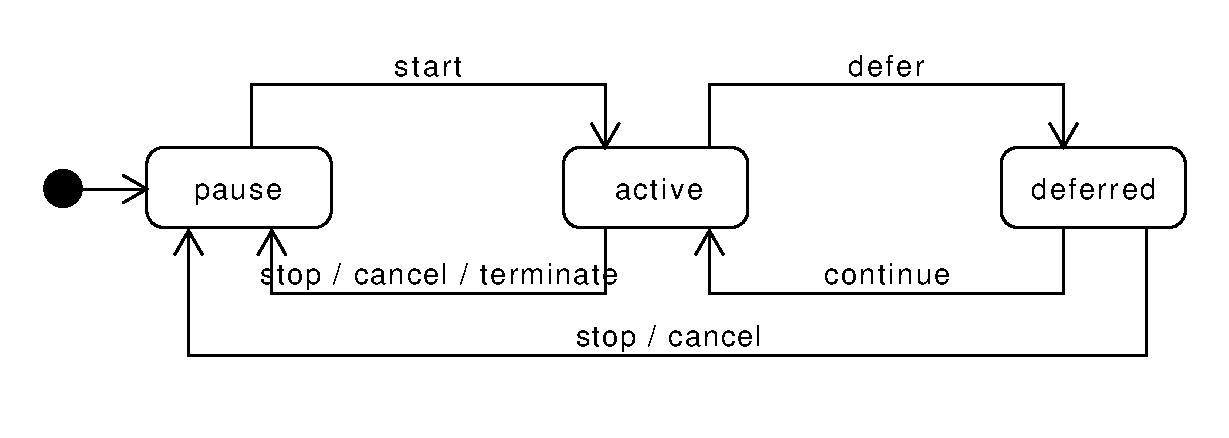
\includegraphics[scale=0.7]{img/Modulkonzeption/FeedbackStateMachine.pdf}
	\caption{Zustandsdiagramm – \emph{InHomeFeedbackModule}}
	\label{fig:feedbackStateMachine}
\end{figure}

\begin{figure}[h!]
	\centering
	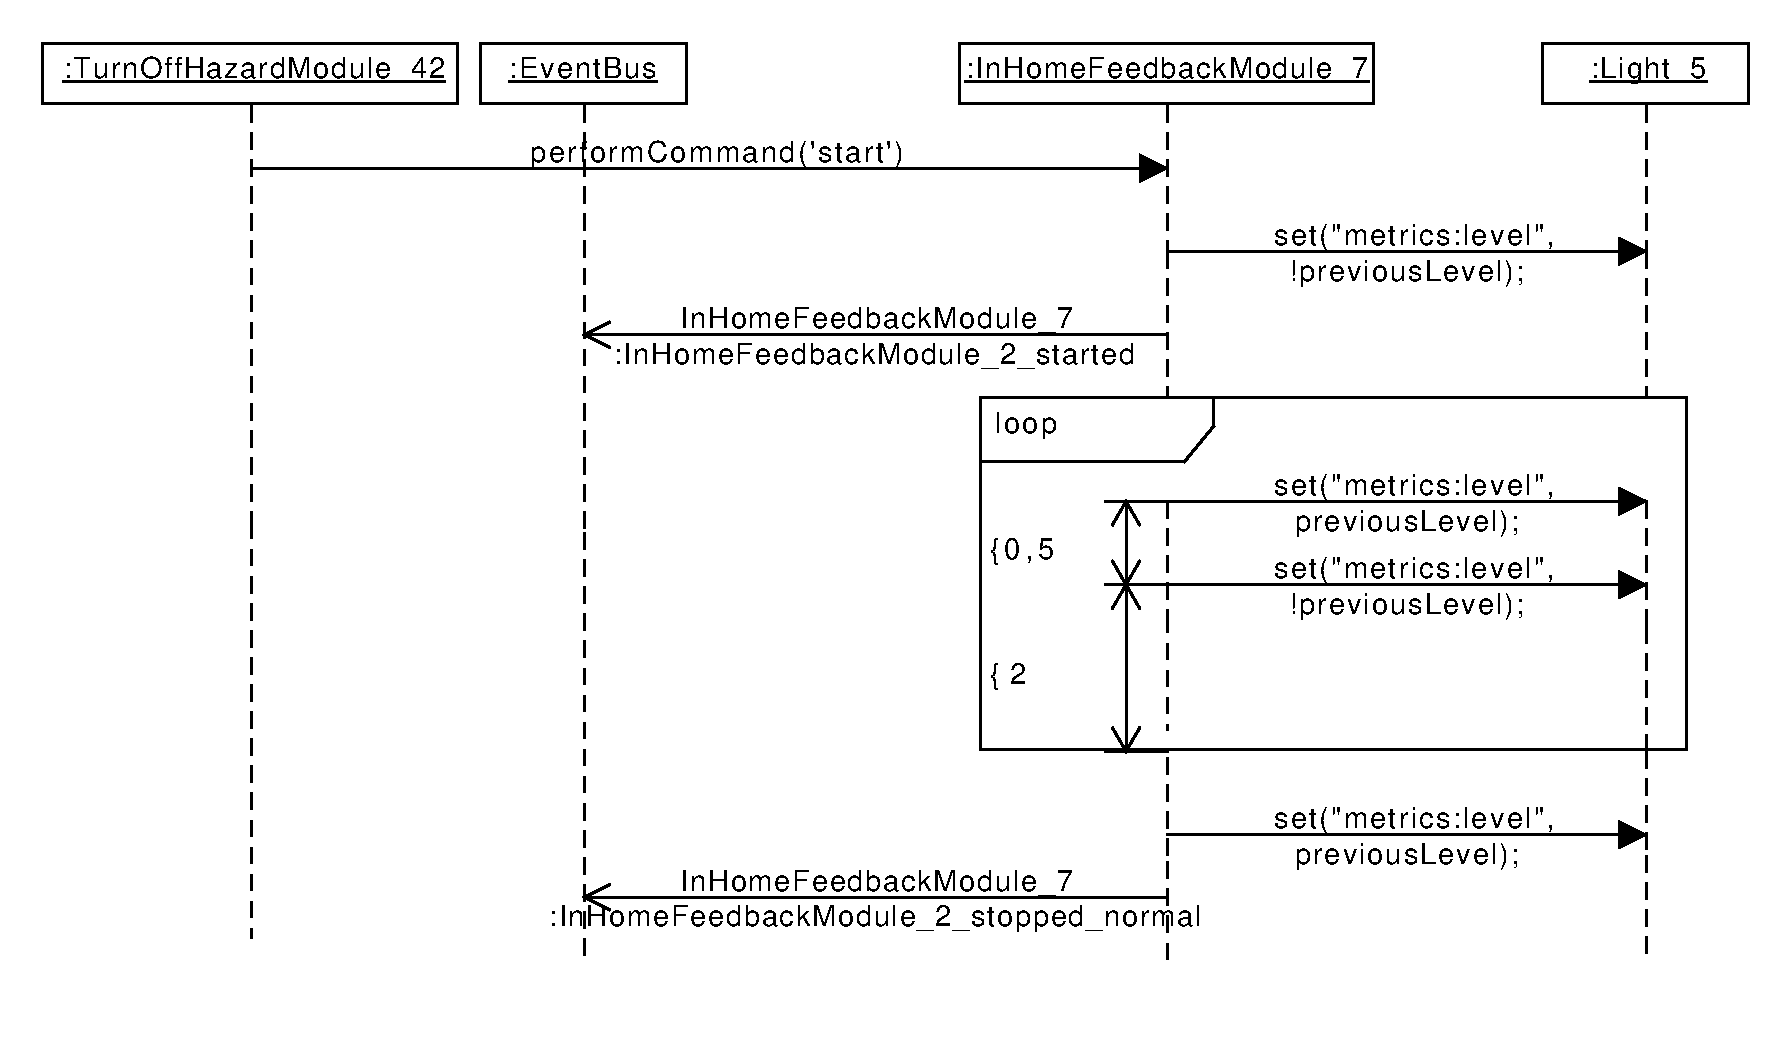
\includegraphics[width=0.9\textwidth]{img/Modulkonzeption/FeedbackSequence.pdf}
	\caption{Sequenzdiagramm – \emph{InHomeFeedbackModule} – Beispiel 1}
	\label{fig:feedbackSequence}
\end{figure}

\begin{figure}[h!]
	\centering
	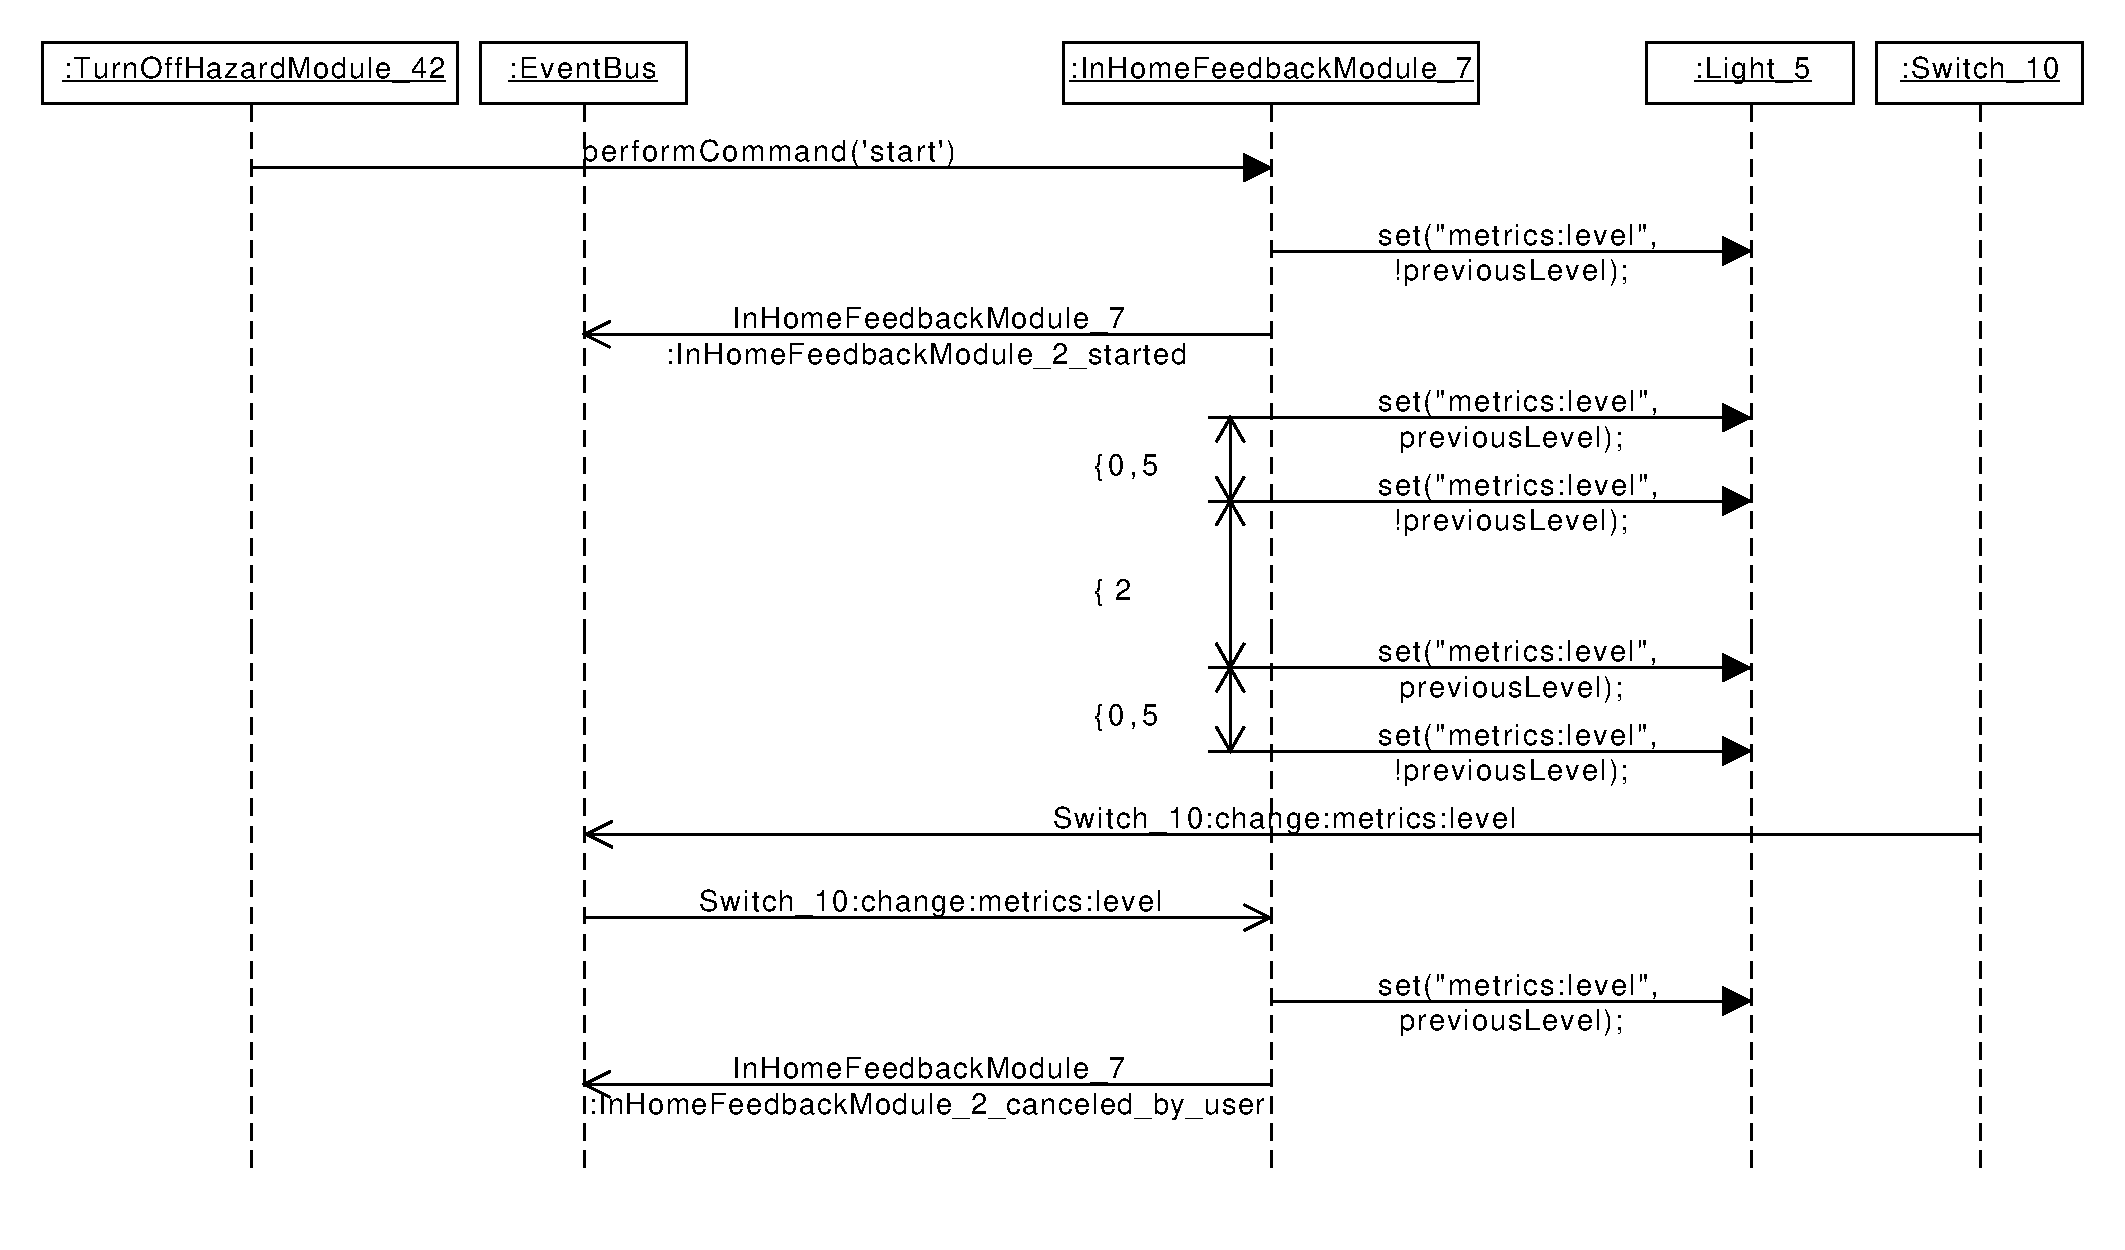
\includegraphics[width=0.9\textwidth]{img/Modulkonzeption/FeedbackSequenceUser.pdf}
	\caption{Sequenzdiagramm – \emph{InHomeFeedbackModule} – Beispiel 2}
	\label{fig:feedbackSequenceUser}
\end{figure}


\subsubsection{Konfiguration}

\begin{itemize}
	\item visuelles Feedback
	\begin{itemize}
		\item Typ: Liste [Binary Switch, Multilevel Switch]
		\item Aktion: an/aus/an/aus/an/... bzw. 0-99-0-99-0-...
		\item erforderlich: nein
		\item Option:
		\begin{itemize}
			\item Frequenz
			\begin{itemize}
				\item Typ: Text
				\item erforderlich: nein
				\item Standard: 5 Sekunden
			\end{itemize}
		\item spezieller Wert, bspw. RGB (RGB + Warmweiß + Kaltweiß)
		\end{itemize}
	\end{itemize}
	\item akustisches Feedback
	\begin{itemize}
		\item Typ: Liste [*] \textrightarrow{ }bspw. Aeon Labs Sirene \textrightarrow{ }Binary Switch
		\item Aktion: an/aus
		\item erforderlich: nein
	\end{itemize}
	\item Nachricht
	\begin{itemize}
		\item Vorbedingung: Auswahl von E-Mail bzw. Push-Nachricht
		\item Typ: Liste [Text] (E-Mail-Adresse bzw. URL)
		\item Aktion: HTTP-Request
		\item erforderlich: nein
	\end{itemize}
	\item Aufruf spezieller Module
	\begin{itemize}
		\item Typ: Liste [Binary Switch, Multilevel Switch] \textrightarrow{ }Device Type der speziellen Module! (deviceType \textrightarrow{ }namespace\_deviceType)
		\item Aktion: an/aus bzw. 0/99
		\item erforderlich: nein
		\item Option:
		\begin{itemize}
			\item spezieller Wert, bspw. RGB (R + G + B + Warmweiß + Kaltweiß)
		\end{itemize}
	\end{itemize}
	\item HTTP
	\begin{itemize}
		\item Typ: Text
		\item erforderlich: nein
	\end{itemize}
	\item JavaScript
	\begin{itemize}
		\item Typ: Text
		\item erforderlich: nein
	\end{itemize}
	\item Raum
	\begin{itemize}
		\item Typ: Text
		\item erforderlich: ja
	\end{itemize}
	\item Dauer (bis automisch deaktiviert)
	\begin{itemize}
		\item Typ: Text
		\item erforderlich: nein
		\item Standard: 30 Sekunden
	\end{itemize}
	\item Verzögerungszeit
	\begin{itemize}
		\item Typ: Text
		\item erforderlich: nein
		\item Standard: 600 Sekunden
	\end{itemize}
	\item Schalter (zum Abbrechen der eingehenden Aktion)
	\begin{itemize}
		\item Typ: Binary Switch
		\item erforderlich nein
	\end{itemize}

\end{itemize}

\subsubsection{Schnittstellen}
%todo tabelle einfügen

\begin{table}[H]
	\begin{tabularx}{\textwidth}{
			>{\hsize=1.25\hsize}X % 40% of 3\hsize 
			>{\hsize=0.5\hsize\centering}X % 30% of 3\hsize
			>{\hsize=1.25\hsize}X % 40% of 3\hsize
			% sum=3.0\hsize for 3 columns
		}
		\hline
		\textbf{URL}						& \textbf{Parameter}	& \textbf{Beschreibung} \\
		\hline 
		/command/start				
				& duration (opt.) \newline endless=true (opt.) 	
						& Starten des Feedback-Modus (die Durchführung der Aktion wird nicht beeinflusst). Der Parameter "`endless=true"' startet den Feedback-Modus, ohne automatische Terminierung nach einer bestimmten Zeitspanne. \\ 
		\hline 
		/command/stop		
				& - 			 		
						& Stoppen des Feedbackmodus (die Durchführung der Aktion wird nicht beeinflusst). \\
		\hline 
		/command/state
				& - 				
						& Liefert den aktuellen Zustand des Moduls. \\
		\hline
		/command/cancel
				& -
						& Die Aktion abbrechen. \\
		\hline
		/command/defer
				& duration (opt.)
						& Die Aktion um eine bestimmte Zeit verschieben. \\
		\hline
	\end{tabularx}
	\caption{\emph{InHomeFeedbackModule}: Schnittstelle ZAutomation}
\end{table}

\begin{table}[H]
	\begin{tabularx}{\textwidth}{
			>{\hsize=1.2\hsize}X 
			>{\hsize=0.8\hsize}X
			% sum=2.0\hsize for 2 columns
		}
		\hline
		\textbf{Event Name}						& \textbf{Beschreibung} \\
		\hline
		[deviceId]:InHomeFeedbackModule\_[roomId]\_started	
				& Feedback-Modus wurde gestartet \\
		\hline 
		[deviceId]:InHomeFeedbackModule\_[roomId]\_stopped\_normal
				& Feedback-Modus wurde nach der vorgegebenen Zeit beendet \\
		\hline
		[deviceId]:InHomeFeedbackModule\_[roomId]\_stopped\_manual
				& Feedback-Modus wurde  gestoppt \\
		\hline
		[deviceId]:InHomeFeedbackModule\_[roomId]\_canceled\_by\_user
				& Feedback-Modus wurde vom Nutzer abgebrochen (aufrufende Komponente sollte dieses Event abfangen und entsprechend reagieren) \\
		\hline
		[deviceId]:InHomeFeedbackModule\_[roomId]\_deferred
				& Aktion wurde um eine bestimmte Zeit aufgeschoben \\
		\hline
		[deviceId]:InHomeFeedbackModule\_[roomId]\_continued
				& - \\
		\hline
	\end{tabularx}
	\caption{\emph{InHomeFeedbackModule}: Schnittstellen Event Bus}
\end{table}

\subsubsection{Abhängigkeiten}
\begin{itemize}
	\item Module, für Geräte von Drittanbietern (Philips Hue, Bose, ...)
\end{itemize}

\subsubsection{Interne Speicher}
\begin{itemize}
	\item Raum ID
	\item Zustand - aktiviert, deaktiviert, aufgeschoben
	\item Dauer - falls Modulkonfiguration für den Command überschrieben
	\item Verzögerungszeit - falls Modulkonfiguration für den Command überschrieben
	
\end{itemize}


\subsection{PersonIdentificationModule}
\emph{(von Martin Petzold)}

\subsubsection{Allgemein}
Das \emph{PersonIdentificationModule} übernimmt die Aufgabe, anhand der Personenanzahl und von Größen- und CO$_2$-Messungen Aussagen darüber zu treffen, ob sich erwachsene Personen oder ausschließlich Kinder im  jeweiligen Raum befinden.

Das \emph{PersonIdentificationModule} erkennt anhand der Messung des CO$_2$-Wertes in einem Raum und einer Größenmessung über eine Höhenmessungsschranke (\prettyref{subsec:groessenerkennungAnTuer}), ob sich in einem Raum eine erwachsene Person befindet oder nicht. Dabei erkennt das Modul Erwachsene nur, wenn beide Messungen entsprechende Ergebnisse liefern.

\subsubsection{Funktionsweise}
Das Modul benötigt ein \emph{PersonCounterModule} für den Raum, in welchem es angewandt wird, da der Abgleich der CO$_2$-Messungen nur in Verbindung des Wissens der Personenanzahl ausgewertet werden kann. Weiterhin erfolgt die Größenmessung in Zusammenhang mit der Änderung der im Raum befindlichen Personenanzahl. Somit ergibt sich die Funktionsweise, dass bei Änderung der Personenanzahl im Raum geprüft wird, ob durch die sich an den Raumzugängen durchgeführten Größenmessungen Erwachsene registriert wurden. Danach beginnt als Abgleich der Größenmessung die Messung der CO$_2$-Änderung im Raum. Haben nach den Messvorgängen beide Messgrößen die Anwesenheit eines Erwachsenen registriert gibt das Modul die Erkennung eines Erwachsenen bekannt. Stellt  allerdings eines der beiden Systeme fest, dass sich kein Erwachsener im Raum befindet, oder alle Erwachsenen den Raum verlassen haben, wird das Signal "`kein Erwachsener erkannt"' gesendet. Dieser Ablauf ist auch im Modell (\prettyref{fig:personIdentification}) dargestellt.

\begin{figure}[h!]
	\centering
	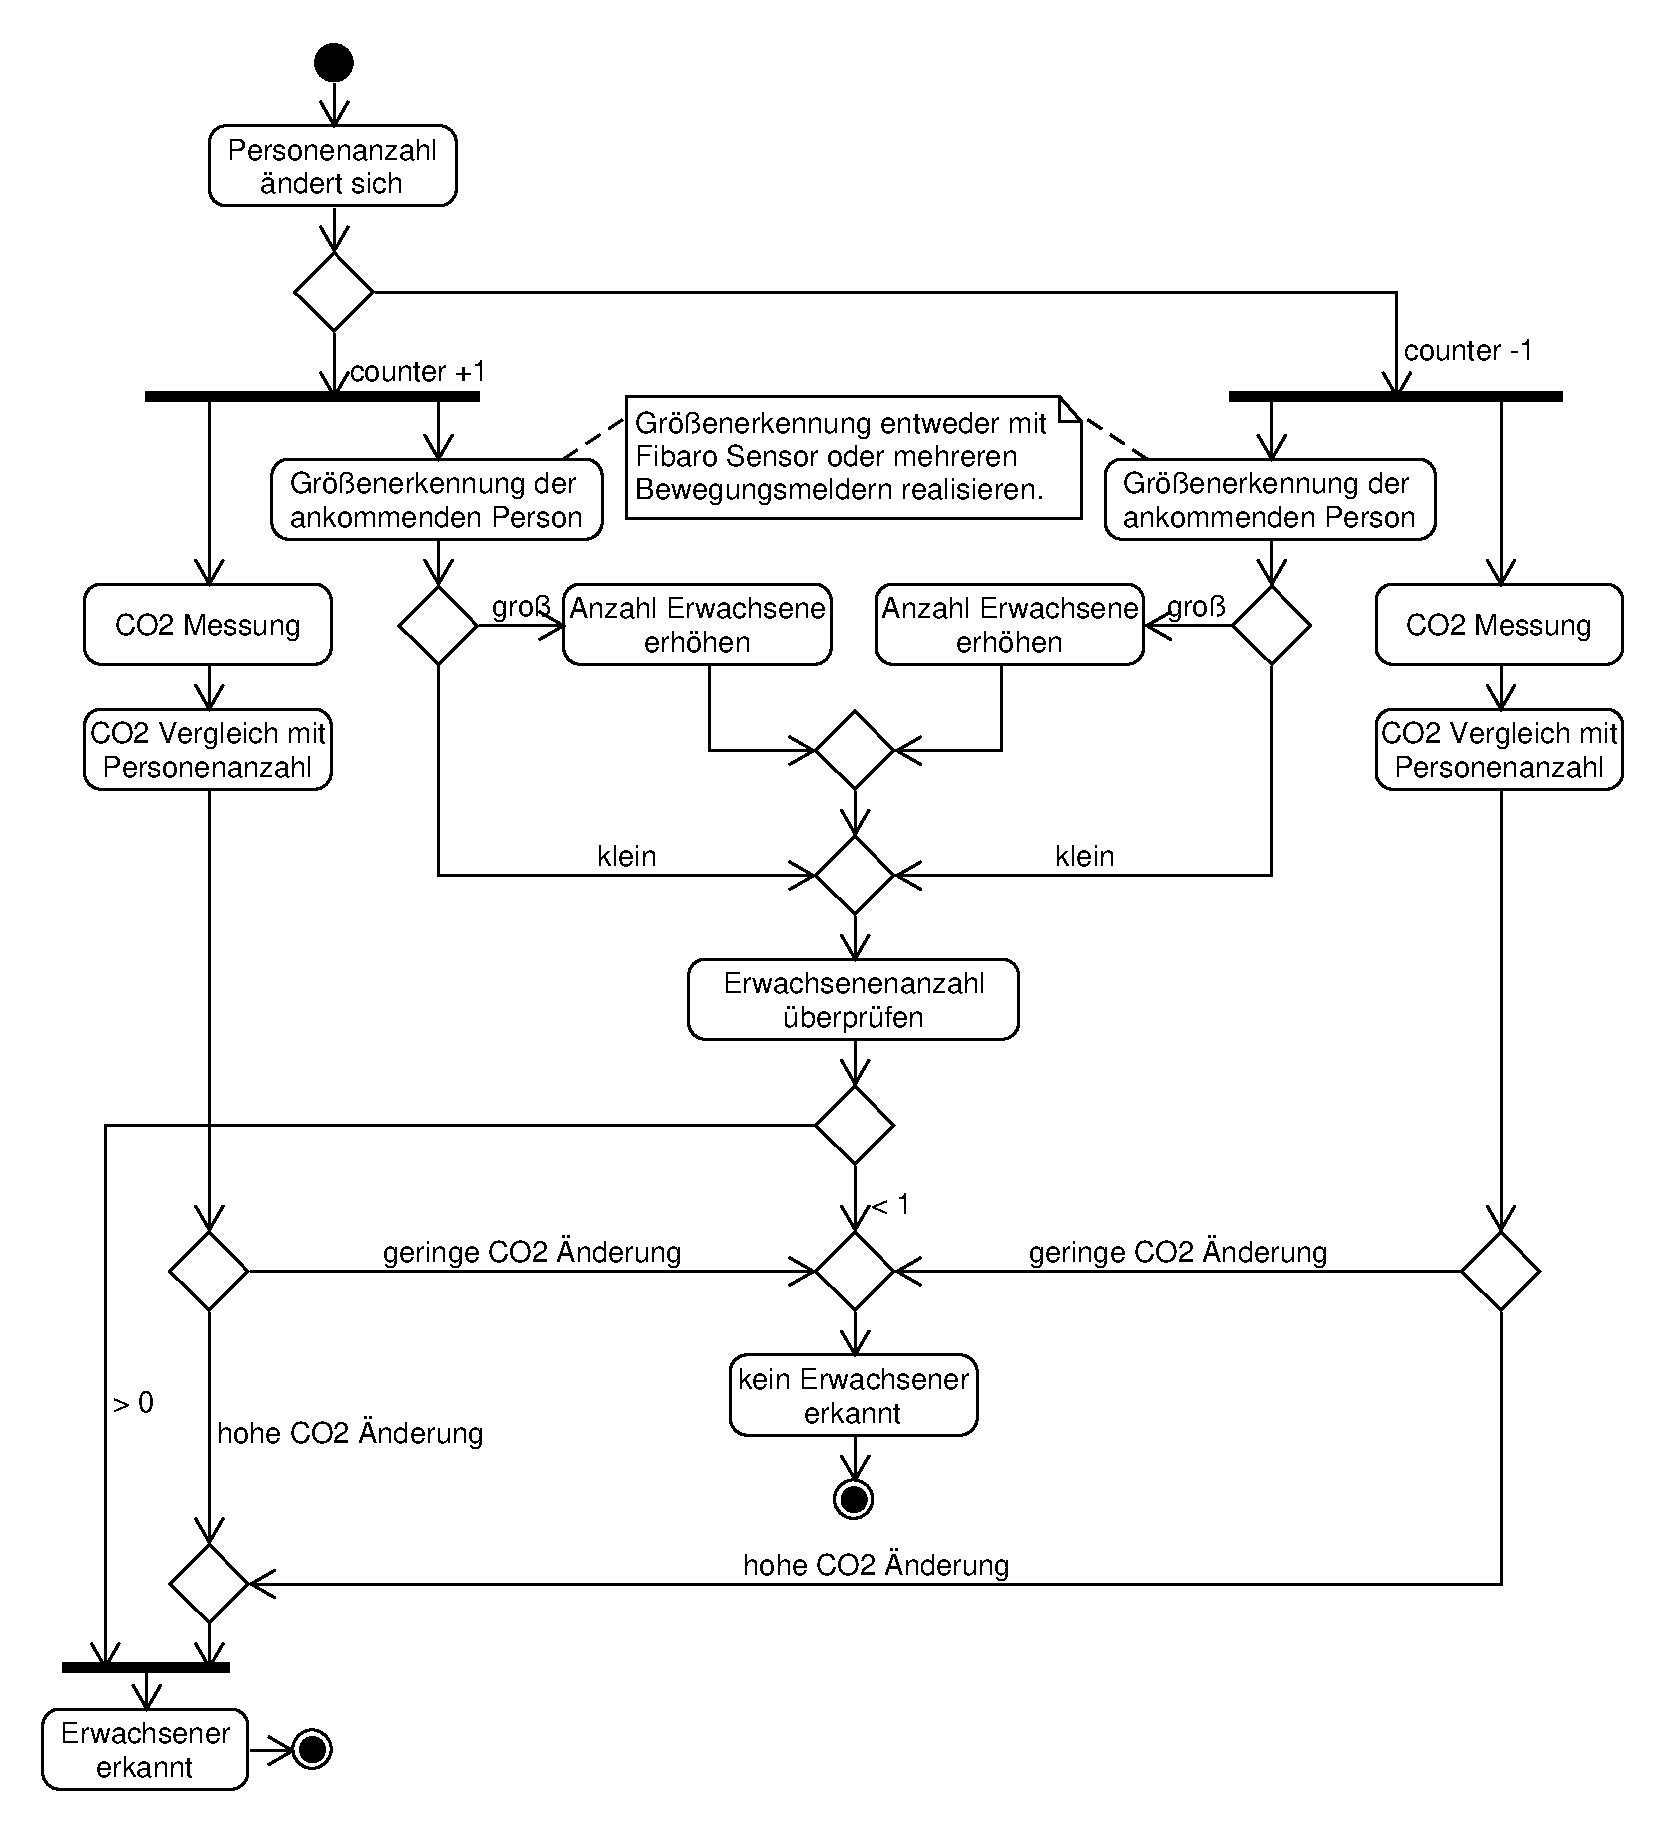
\includegraphics[width=0.9\textwidth]{img/Modulkonzeption/PersonIdentificationStateMachine.pdf}
	\caption{\emph{PersonIdentificationModule} - Zustandsdiagramm}
	\label{fig:personIdentification}
\end{figure}

\paragraph{CO$_2$-Messung} Das Modul startet die CO$_2$-Messung, wenn:

\begin{enumerate}
	\item das modulinterne "`runningState"' auf "`true"' gesetzt ist
	\item das modulinterne Messdatenobjekt initialisiert wurde
	\item alle Tür- und Fensterkontakte geschlossen sind
	\item der CO$_2$-Sensor einen ersten Messwert sendet
\end{enumerate}

Danach werden in einem bestimmten Intervall die vom CO$_2$-Sensor gesendeten Daten aufgenommen. Nachdem die Messwerte aufgenommen wurden, wird, um Messungenauigkeiten auszugleichen, durch die \gls{mkq} eine Geradenfunktion anhand der Messwerte erstellt. Nachdem diese Funktion errechnet wurde, wird anhand der Zeitpunkte des ersten und des letzten Messpunktes eine CO$_2$-Differenz bestimmt (\prettyref{fig:personIdentificationChart}).

\begin{figure}[h!]
	\centering
	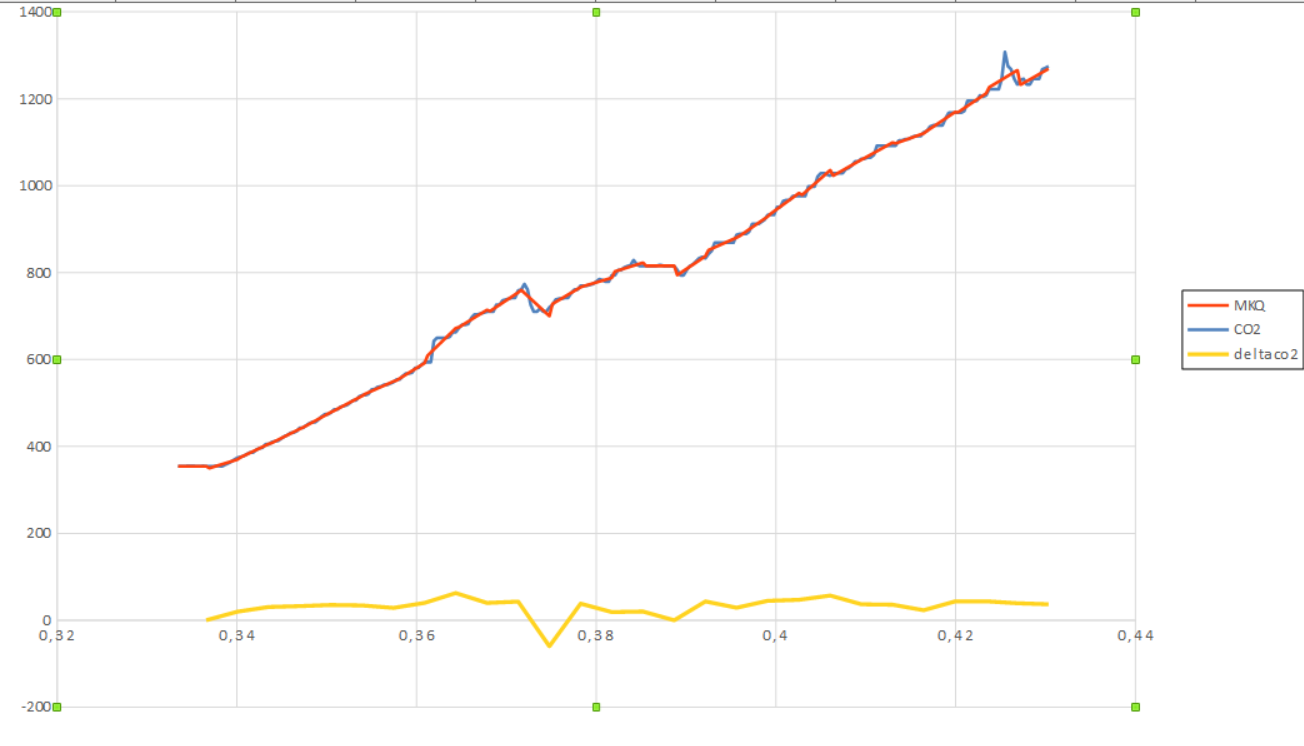
\includegraphics[width=0.9\textwidth]{img/Modulkonzeption/PersonIdentificationChart.png}
	\caption{Erfassung und Mittlung der CO$_2$-Werte}
	\label{fig:personIdentificationChart}
\end{figure}

\paragraph{Zeitraum für Messungen}
Der Wert von einer Minute Wartezeit pro 25.000 Liter Raumvolumen ist ein Erfahrungswert, der sich aus Probemessungen und der Beispielrechnung nach dem intellexi Standardlehraussagen Stand 2014 ergibt\footnote{\url{http://projektserver.informatik.fh-zwickau.de/attachments/download/4128/BerechnungenundTabellenCO2BerbrauchMensch.pdf}}. Wobei davon Ausgegangen wird, dass innerhalb dieser Zeitspanne eine Unterscheidung des CO$_2$-Verbrauchs von Kindern und Erwachsenen möglich ist.

\paragraph{Höhenmessung}
Die Höhenmessung des Moduls vergleicht die Zeitpunkte der letzten Änderung des dem Modul zugeordneten \emph{PersonCounters} und der Sensoren zur Höhenmessung. Wenn innerhalb eines Zeitraumes ("`highmeasureWaitingtime"') in Sekunden gleichzeitig eine Höhenerkennung und eine Änderung des \emph{PersonCounters} erfolgt, wird ein Erwachsener erkannt. Der, wenn der \emph{PersonCounter} sich verringert, vom "`adultCounter"' abgezogen und wenn er sich erhöht auf den "`adultCounter"' addiert wird.

\paragraph{Vergleich der Messungen}
Sobald die CO$_2$-Differenz bestimmt wurde, wird dessen Ergebnis mit der Personenanzahl und den Angaben zu den Personae verrechnet. Dabei wird verglichen, ob das CO$_2$-Delta den Standardwert für den maximalen CO$_2$-Verbrauch für Kinder der gleichen Anzahl Personen im Raum übersteigt. Ist der Verbrauch im Raum höher, gibt die CO$_2$-Messung ihr "`OK"', dass ein Erwachsener erkannt wurde. Ist sowohl dieses Ok gegeben als auch der "`AdultCounter"' der Höhenmessung größer 1, schaltet das Modul auf "`on"', ansonsten bleibt es "`off"'.

\paragraph{Abbruchbedingungen und Reinitialisierung}
Es gibt mehrere Bedingungen, welche die momentanen Messdaten zurücksetzen und neu starten. Daraufhin gibt das Modul seinen aktuellen Status über den Event Bus bekannt. Diese Bedingungen sind:
\begin{enumerate}
	\item der zugehörige \emph{PersonCounter} ändert sich
	\item ein Fenster- oder Tür-/Sensorkontakt schaltet "`off"'
	\item eine CO$_2$-Messung ist abgeschlossen und wurde ausgewertet
\end{enumerate}

\paragraph{Neue Commands}
Gegen Ende der Entwicklung wurde eine Schnittstelle entwickelt, welche es ermöglicht, die CO$_2$-Messung zu deaktivieren. Infolge dessen wird die Erkennung von Erwachsenen nur anhand der Höhenmessung durchgeführt.

\paragraph{CO$_2$-Sensor Korrekturfaktor}
Diese Einstellmöglichkeit des Moduls ermöglicht es, die Messwerte des CO$_2$-Sensors anzupassen. Das ist notwendig, da die CO$_2$-Werte, welche zur Berechnung der Schwellwerte für das Volumen eines idealen Raumes berechnet werden.

Ein idealer Raum ist dadurch definiert, dass er keinen Luftaustausch mit der Umgebung hat, nicht mit Möbeln bestückt ist und die Luft im Raum gleichmäßig umgewälzt wird. Da diese Faktoren meist nicht gegeben sind, wird der Korrekturfaktor dazu genutzt, diese konstanten Abweichungen auszugleichen. Es wäre weiterhin denkbar, statt des Korrekturfaktors eine Kalibrierung zu benutzen.

\subsubsection{Konfiguration}
\begin{itemize}
	\item CO$_2$-Sensor
	\begin{itemize}
		\item Typ: Multilevel Sensor
		\item erforderlich: ja
		\item Ausgabewert: CO$_2$-Gehalt in ppm
	\end{itemize}
	\item doorWindowContacts
	\begin{itemize}
		\item Typ: Liste[Binary Switches]
		\item erforderlich: ja
		\item Ausgabewert: true/false
	\end{itemize}
	\item peopleSizeMeasurement 
	\begin{itemize}
		\item Typ: Liste[Binary Switches]
		\item erforderlich: ja
		\item Ausgabewert: true/false
	\end{itemize}
	\item roomHeight
	\begin{itemize}
		\item Typ: integer
		\item erforderlich: ja
	\end{itemize}
	\item roomWidth
	\begin{itemize}
		\item Typ: integer
		\item erforderlich: ja
	\end{itemize}
	\item roomLength
	\begin{itemize}
		\item Typ: integer
		\item erforderlich: ja
	\end{itemize}
	\item roomId
	\begin{itemize}
		\item Typ: integer
		\item erforderlich: ja
	\end{itemize}
	\item correctionFactor
	\begin{itemize}
		\item Typ: integer
		\item erforderlich: ja
	\end{itemize}
	\item personCounter
	\begin{itemize}
		\item Typ: Metrik
		\item erforderlich: ja
	\end{itemize}
\end{itemize}

\subsubsection{Schnittstellen}
\begin{table}[H]
	\begin{tabularx}{\textwidth}{
			>{\hsize=1.25\hsize}X % 40% of 3\hsize 
			>{\hsize=0.5\hsize\centering}X % 30% of 3\hsize
			>{\hsize=1.25\hsize}X % 40% of 3\hsize
			% sum=3.0\hsize for 3 columns
		}
		\hline
		\textbf{URL}						& \textbf{Parameter}	& \textbf{Beschreibung} \\
		\hline 
		/command/areThereAdults				
		& - 	
		& Gibt ein Boolean zurück ob sich im Raum Erwachsene befinden. \\ 
		\hline 
		/command/setPersons		
		& Anzahl, Erwachsenenanzahl		% TODO: wie heißen die Parameter wirklich?	 		
		& Setzt die Anzahl der Personen im Raum und startet C02-Messung. \\
		\hline 
		/command/giveData
		& - 				
		& Gibt die Personen-, Erwachsenen- und Kinderanzahl an, die das System registriert hat. \\
		\hline
		/command/setCorrectionFactor
		& Factor
		& Korrekturfaktor für die CO$_2$-Messung. \\
		\hline
		/command/setMeasureTimeDelta
		& TimeDelta
		& Zeitabstand zwischen Änderung des PersonCounter und Höhenmessung, welche noch einen Zusammenhang darstellen. \\
		\hline
		/command/start
		& -
		& \\
		\hline
		/command/stop
		& - 
		& \\
		\hline
		/command/debugOn
		& - 
		& \\
		\hline
		/command/debugOff
		& - 
		& \\
		\hline
	\end{tabularx}
	\caption{PersonIdentification: Schnittstelle ZAutomation}
\end{table}

\begin{table}[H]
	\begin{tabularx}{\textwidth}{
			>{\hsize=1.2\hsize}X 
			>{\hsize=0.8\hsize}X
			% sum=2.0\hsize for 2 columns
		}
		\hline
		\textbf{Event Name}						& \textbf{Beschreibung} \\ %TODO Beschreibung einfügen?
		\hline
		[deviceId]:PersonIdentificationModule\_[roomId]\_started	
		& - \\
		\hline 
		[deviceId]:PersonIdentificationModule\_[roomId]\_stoped
		& - \\
		\hline
		[deviceId]:PersonIdentificationModule\_[roomId]\_adult\_there
		& - \\
		\hline
		[deviceId]:PersonIdentificationModule\_[roomIId]\_no\_adult\_there
		& - \\
		\hline
	\end{tabularx}
	\caption{PersonIdentification: Schnittstellen Event Bus}
\end{table}

\subsubsection{Abhängigkeiten}
\begin{itemize}
	\item \emph{PersonCounterModule}
\end{itemize}

\subsubsection{Interne Speicher}

\begin{table}[H]
	\begin{tabularx}{\textwidth}{
			>{\hsize=0.85\hsize}X 
			>{\hsize=0.85\hsize}X
			>{\hsize=1.45\hsize}X
			>{\hsize=0.85\hsize}X
			% sum=2.0\hsize for 2 columns
		}
		\hline
		\textbf{Speicher Name}	& \textbf{Datentyp}		& \textbf{Beschreibung}		& \textbf{Initialwert} \\
		\hline
		level					& integer				& Entsprechung des Status "`off"' ist false und "`on"' ist true.	& off \\
		\hline
		status					& boolean				& Status true wenn Erwachsener erkannt, false wenn nicht oder Zustand undefiniert.	& false \\
		\hline
		personCount				& integer				& Interner Zwischenspeicher der Personenanzahl vom zugehörigen Personcounter.	& 0 \\
		\hline
		adultCount				& integer				& Erkannte Erwachsene, welche durch die Größenmessung erkannt wurden.	& 0 \\
		\hline
		room					& integer				& RoomId																& -1 \\
		\hline
		correctionFactor		& integer				& Konstante zur Korrektur,  welche  mit  Messungen multipliziert wird.	& 1 \\
		\hline
		runningState			& boolean				& Zustand ob die Messungen ausgewertet werden oder nicht.			& true \\ 
		\hline
	\end{tabularx}
	\caption{PersonIdentification: Interne Speicher}
\end{table}


\subsection{TurnOffTimerModule}
\emph{(von Tobias Weise)}
\subsubsection{Funktionsweise}
Das \emph{TurnOffTimerModule} übernimmt die Aufgabe, nach einem eingehenden Command mit der Angabe der Ablaufdauer und einer zugewiesenen Priorität, einen Timer zu starten. Nach Ablauf oder Unterbrechung des Timers wird ein entsprechendes Event an den Event Bus verschickt. 

Ein \emph{TurnOffTimerModule} enthält zusätzlich die Information, für welchen Raum es bestimmt ist. Somit kann es beliebig oft innerhalb eines Raumes verwendet werden.

\subsubsection{Schnittstellen}

\begin{longtabu} to \textwidth{
		>{\hsize=1.25\hsize}X % 40% of 3\hsize 
		>{\hsize=0.5\hsize\centering}X % 30% of 3\hsize
		>{\hsize=1.25\hsize}X % 40% of 3\hsize
		% sum=3.0\hsize for 3 columns
	}
	\hline
	\textbf{URL}						& \textbf{Parameter}	& \textbf{Beschreibung} \\
	\hline
	\endhead
	/command/start\_timer				& time 					& Starten des Timers, für die Länge der angegebenen Dauer in Sekunden. \\ 
	\cline{2-3}
										& priority		 		& Für den Timerstart muss eine Priorität angegeben werden. Je höher der Wert, desto höher die Priorität. \\
	\hline 
	/command/stop						& -						& Stoppen des Timers. \\
	\hline
	\caption{\emph{TurnOffTimerModule}: Schnittstelle ZAutomation}
\end{longtabu}

\begin{longtabu} to \textwidth{
		>{\hsize=1.25\hsize}X 
		>{\hsize=0.75\hsize}X
	}
	\hline
	\textbf{Event Name}									& \textbf{Beschreibung} \\
	\hline
	\endhead
	[DeviceId]:TurnOffTimerModule\_[RaumId]\_expired	& Benachrichtigung, wenn die Zeit des Timers abgelaufen ist. \\ 
	\hline 
	[DeviceId]: TurnOffTimerModule\_[RaumId]\_canceled	& Benachrichtigung, wenn der Zeitablauf unterbrochen wurde. \\
	\hline
	\caption{\emph{TurnOffTimerModule}: Schnittstelle Event Bus}
\end{longtabu}
	
\subsubsection{Abhängigkeiten}
\begin{itemize}
	\item \emph{InHomeFeedbackModule}: wenn der Timer aktiviert wurde, wird auch das Nutzerfeedback gestartet und falls durch Nutzerinteraktion das \emph{Feedbackmodul} unterbrochen wird, wird der Timer ebenfalls abgebrochen	
\end{itemize}


\subsubsection{Interne Speicher}
\begin{itemize}
	\item Raum ID
	\item Variable "`cancel"': "`1"' wenn der Timer unterbrochen wurde, "`0"' sonst
\end{itemize}

\subsubsection{Einsatzmöglichkeiten}
Der \emph{TurnOffTimer} wurde für das Projekt so erstellt, dass nur eine Instanz des Timers für jeden Raum genutzt werden kann. Anhand der Prioritäten ist es jedoch möglich, mit den entsprechenden Timer-Commands eine bestimmte Wichtigkeit zu definieren. Dabei ist zu beachten, dass ein höherer Zahlenwert eine höhere Priorität bedeutet. Nachfolgende Abbildung (\prettyref{fig:turnOffTimer}) soll das Verhalten des Timers bei entsprechender Priorisierung näher verdeutlichen.

\begin{figure}[h!]
	\centering
	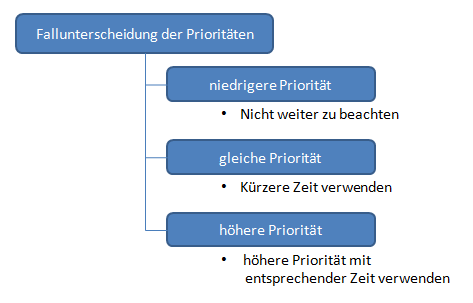
\includegraphics[width=0.5\textwidth]{img/Modulkonzeption/TurnOffTimer.png}
	\caption{Übersicht Prioritätenverhalten}
	\label{fig:turnOffTimer}
\end{figure}

Eine andere Möglichkeit zur Integration des Timers besteht darin, dass jedes Modul, welches pro notwendigen Raum definiert wird, eine eigenständige Instanz des Timers erzeugt. Dieser instanziierte Timer existiert anschließend solange, wie dieses Modul ihn für eine Timerlaufzeit benötigt.


\subsection{TurnOffHazardModule}
\emph{(von Patrick Hecker und Tobias Weise)}

\subsubsection{Allgemein}
Das \emph{TurnOffHazardModule} übernimmt die Aufgabe, eine vom Nutzer individuell erstellbare Liste an Gefahrenquellen zu speichern. Daraufhin soll das Modul in einem zuvor definierten Fehlerfall alle Gefahrenquellen, die in der Liste aufgeführt sind, abschalten bzw. eine spezielle Aktion ausführen. Um definieren zu können, wann ein Fehlerfall vorliegt, wird in dem Modul die Anzahl der Kinder, der Erwachsenen und der Personen im Raum allgemein registriert. Das Abschalten der Geräte erfolgt jedoch nicht direkt. Ein Abschalttimer für den Raum ermöglicht anwesenden Personen die Aktion abzubrechen.

Ein \emph{TurnOffHazardModule} enthält zusätzlich die Information, für welchen Raum es bestimmt ist.

\subsubsection{Funktionsweise}
Ein Beispielablauf könnte sein, dass eine erwachsene Person den Raum verlässt. Daraufhin wird der \emph{PersonCounter} und das \emph{PersonIdentificationModule} aktiv, um nach einer internen Berechnung, die Information, dass ein Erwachsener den Raum verlassen hat, anderen Modulen zur Verfügung zu stellen.

Das \emph{TurnOffHazardModule} registriert dieses Ereignis und beginnt sofort mit der Abschaltroutine, indem es den \emph{TurnOffTimer} startet. In diesem Beispiel wird angenommen, dass sich keine weitere Person im Raum befindet und der Abschalttimer ohne Abbruch abläuft. Nach Ablauf benachrichtigt der Abschalttimer das \emph{TurnOffHazardModule}, welches die konfigurierten Gefahrenquellen abschaltet.

Dieses Beispielszenario ist nachfolgend in einem Sequenzdiagramm modelliert wurden.

\begin{figure}[h!]
	\centering
	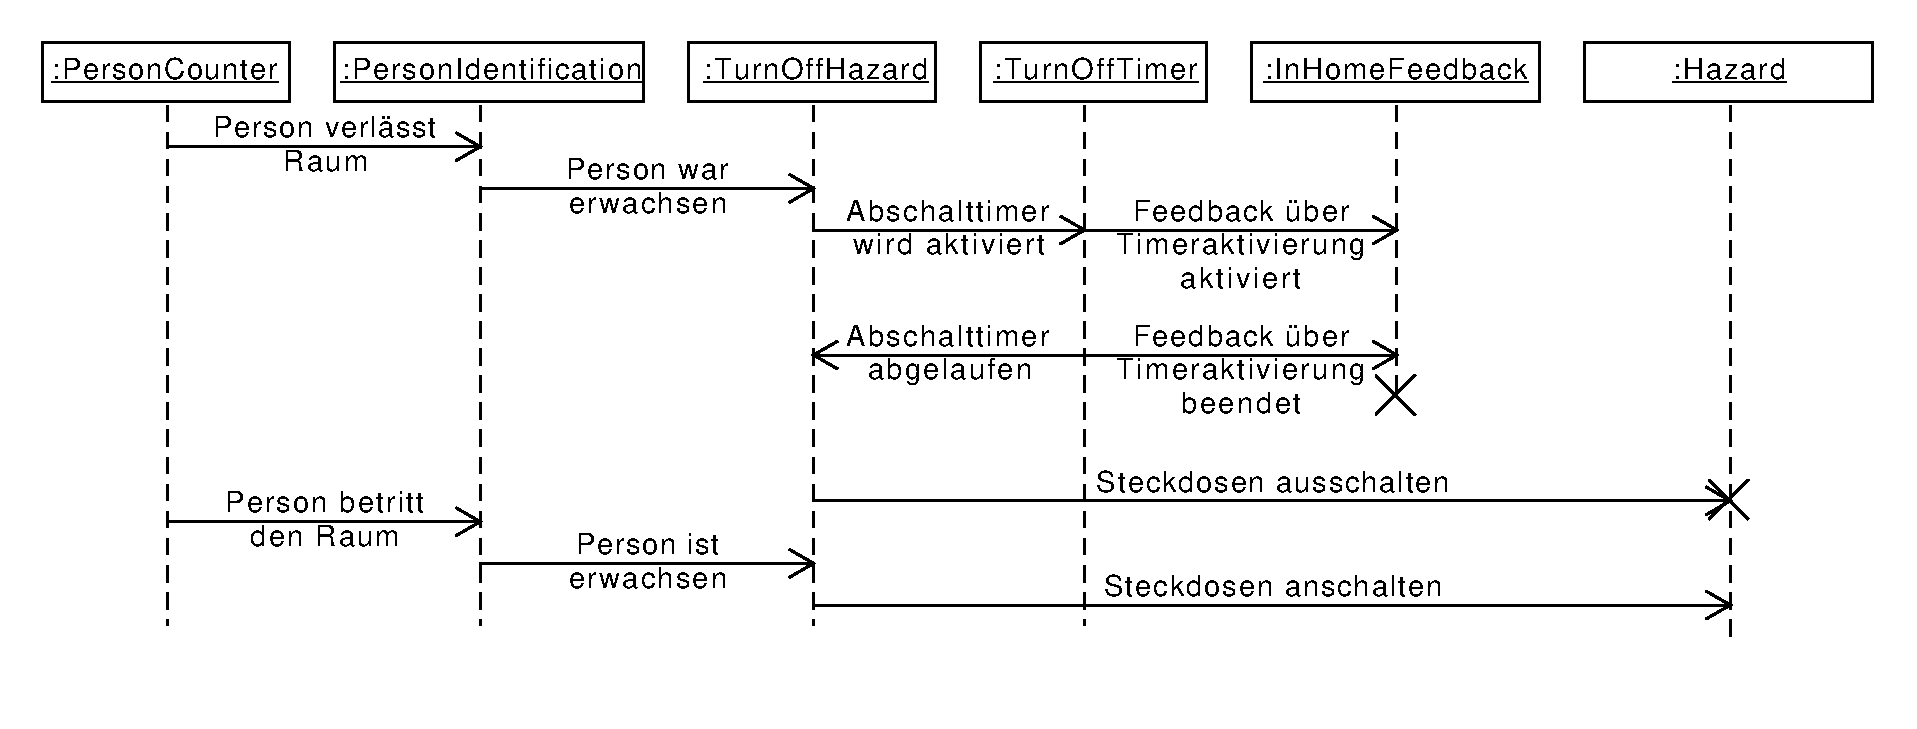
\includegraphics[width=\textwidth]{img/Modulkonzeption/TurnOffHazardSequence.pdf}
	\caption{\emph{TurnOffHazardModule}: Sequenzdiagramm}
	\label{fig:turnOffHazard}
\end{figure}

\subsubsection{Konfiguration}
\begin{itemize}
	\item Gefahrenquellen
	\begin{itemize}
		\item Typ: Liste [Binary Switch, Multilevel Switch]
		\item Aktion: definierte Aktion beim Abschalten bzw. Einschalten
		\item erforderlich: ja
	\end{itemize}
	
	\item Dauer (bis automatisch deaktiviert)
	\begin{itemize}
		\item Typ: Text
		\item erforderlich: ja
		\item Default: 60 s
	\end{itemize}
	
	\item Priorität (beim Starten des \emph{TurnOffTimerModule})
	\begin{itemize}
		\item Typ: Text
		\item erforderlich: nein
		\item Default: 5
	\end{itemize}
	
	\item Raum ID
	\begin{itemize}
		\item Typ: Text
		\item erforderlich: ja
	\end{itemize}
\end{itemize}

\subsubsection{Schnittstellen}
\begin{longtabu} to \textwidth{
		>{\hsize=0.8\hsize}X
		>{\hsize=1.2\hsize}X
	}
	% ----------- begin header -----------
	\hline
	\textbf{URL}				& \textbf{Beschreibung} \\
	\hline
	\endhead
	% ----------- end header -----------
	
	% ----------- begin footer -----------
	\multicolumn{2}{r}{{Fortsetzung auf nächster Seite}}  \\
	\endfoot
	\endlastfoot
	% ----------- end footer -----------
	/command/hazardOff			& Abschalten aller Gefahrenquellen aus der Liste. \\
	\hline
	/command/hazardOn			& Einschalten aller Gefahrenquellen aus der Liste. \\
	\hline 
	/command/state				& Liefert den aktuellen Zustand des Moduls. \\
	\hline
	/command/history			& Liefert eine Liste mit den Zeitpunkten und deren Begründung nach abgeschalteten Gefahrenquellen. \\
	\hline
	
	\caption{\emph{TurnOffHazardModule}: Schnittstelle ZAutomation}
\end{longtabu}

\subsubsection{Abhängigkeiten}
\begin{itemize}
	\item Module für Geräte von Drittanbietern
	\item \emph{TurnOffTimerModule} zum Starten und Stoppen des \emph{TurnOffTimerModule}
	\item \emph{PersonCounterModule} zum Erfassen der Personenzahlen im Raum
	\item \emph{PersonIdentificationModule} zum Erfassen der Kinder und Erwachsenen im Raum
\end{itemize}

%TODO: deutsche Modulnamen?

\subsubsection{Interne Speicher}
\begin{itemize}
	\item Raum ID
	\item Liste aller Gefahrenquellen
	\item Dauer eines aktivierten \emph{TurnOffTimerModules}
	\item Priorität beim Starten des \emph{TurnOffTimerModules}
	\item Anzahl der Kinder im Raum
	\item Anzahl der Erwachsenen im Raum
	\item Anzahl der Personen im Raum
	\item Zustand des zugehörigen \emph{TurnOffTimerModules}
	\item Historie zum Speichern der Abschaltzeiten und Abschaltbegründung der Gefahrenquellen
\end{itemize}

%%%%%%%%%%%%%%%%%%%%%%%%%%%%%%%%%%%%%%%%%%%%%%%%%%%%%%%%%%%%%%%%%%%%%%%%%%%%%%%%
\section{Auswahl der Sensoren}
\label{sec:sensorAuswahl}
\emph{(von Simon Schwabe)}

\subsection{Voraussetzungen bei der Auswahl}
Zu Beginn des Projekts standen noch keine Sensoren für die Arbeit und Entwicklung zur Verfügung. Es ist deshalb erforderlich, eine Auswahl an Sensoren zu treffen, welche bestmöglich geeignet ist, die erarbeiteten Szenarien zu realisieren. Für die Sensoren besteht Wahlfreiheit, allerdings müssen einige Rahmenbedingungen beachtet werden.

\begin{enumerate}
	\item Im Rahmen des Projekts wird ausschließlich mit der Z-Wave-Funktechnologie gearbeitet.
	\item Sensoren sollten über den Händler Z-Wave Europe\footnote{\url{http://new.zwave.eu/index.php?id=13\&L=0}} erhältlich sein, da mit diesem Unternehmen im Rahmen eines anderen Projekts zusammengearbeitet wird.
	\item Die Gesamtkosten für die Sensoren sollten 500 € nicht übersteigen.
\end{enumerate}

\subsection{Recherche und Auswahl}
Zwar existiert auf den ersten Blick eine Vielzahl an Geräten, bei genauerer Betrachtung fällt allerdings auf, dass nur wenige verschiedene Kategorien von Sensoren existieren. (Tür- und Fensterkontakte, Überflutungssensoren, Rauchmelder, Bewegungsmelder, Temperatur"~, Helligkeit"~, UV- und Vibrationssensoren)
% ("~ prevents hyphenation)

Die meisten erhältlichen Geräte stellen nicht nur einen Sensor zur Verfügung, sondern bieten eine Kombination verschiedener Sensoren. In diesem Projekt sollen Sensoren eingesetzt werden, um die Anwesenheit von Personen zu erkennen. Deshalb sind Rauch- und Überflutungssensoren nicht hilfreich.

Bewegungsmelder sind die am Besten geeigneten Sensoren zur Erkennung von Personen. Deshalb wurden Bewegungsmelder in drei verschiedenen Ausprägungen in die Auswahl aufgenommen. Es wurden verschiedene Modelle gewählt, um deren Leistungsfähigkeit und Funktionsumfang bestmöglich untersuchen und vergleichen zu können.

Eine besondere Stellung nimmt der CO$_2$-Sensor ein. Zum einen ist er kostenintensiver, zum anderen ist im Voraus nicht bekannt, ob er geeignet ist, die Anwesenheit von Personen anhand des CO$_2$ Ausstoßes zu erkennen und verschiedene Persona (Kinder, Erwachsene) zu identifizieren.

In Ergänzung zum CO$_2$-Sensor wurde ein Tür- und Fensterkontakt ausgewählt. Dieser ist nützlich, um feststellen, ob ein Fenster geöffnet ist. Ist das der Fall, werden die CO$_2$-Werte verfälscht und besitzen unter Umständen keine Aussagekraft.

Die folgende Tabelle gibt einen Überblick der erworbenen Sensoren sowie deren  Messgegenstand. Um ein Z-Wave-Netzwerk aufzubauen, ist ein Z-Wave-Funktransceiver erforderlich, dazu wird ein entsprechender USB-Stick genutzt. Zur direkten Interaktion mit dem Netzwerk wurde ein Popp Wall Controller (Wandschalter) gewählt. Dieser ermöglicht die Steuerung von Geräte und stellt die direkteste Form der Interaktion für den Bewohner dar. Exemplarisch für viele Geräte, welche über Z-Wave angesprochen und gesteuert werden können, wurde eine schaltbare Steckdose gewählt. Diese kann programmatisch an- und abgeschaltet und die Farbe des LED-Ring geändert werden.

\subsection{Übersicht bestellter Sensoren}

\begin{longtabu} to \linewidth {
		>{\hsize=1.1\hsize}X
		>{\hsize=0.5\hsize}X
		>{\hsize=1.1\hsize}X
		>{\hsize=1.3\hsize}X
		% sum=2.0\hsize for 2 columns
	}
	% ----------- begin header -----------
	\hline
	\textbf{Abbildung}			& \textbf{Preis}		& \textbf{Produktname, Bestellnummer}		& \textbf{Messgegenstand, Bemerkung} \\
	\hline
	\endhead
	% ----------- end header -----------

	% ----------- begin footer -----------
	\multicolumn{4}{r}{{Fortsetzung auf nächster Seite}}  \\
	\endfoot
	\endlastfoot
	% ----------- end footer -----------

	\vspace{0cm}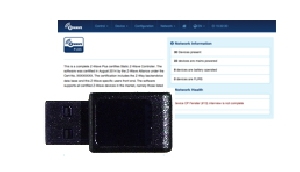
\includegraphics[width=0.24\textwidth]{img/Sensorauswahl/UZB.jpeg}
	& 94,01 €
	& USB Stick inkl. Z-Way Controller Software \newline \textbf{ZMEEUZBWAY}
	& - \\
	\hline
	\vspace{0cm}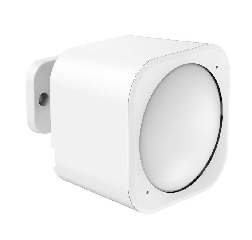
\includegraphics[width=0.24\textwidth]{img/Sensorauswahl/Aeotec.jpg}
	& 64,99 €
	& Z-Wave Multisensor 6 \newline \textbf{AEOEZW100}
	& Bewegung, Temperatur, Vibration, UV, Luftfeuchtigkeit \\
	\hline
	\vspace{0cm}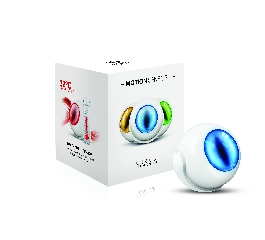
\includegraphics[width=0.24\textwidth]{img/Sensorauswahl/FibaroMulti.jpg}
	& 56,99 €
	& Z-Wave Multisensor \newline \textbf{FIB\_FGMS-001}
	& Bewegung, Temperatur, Licht \\
	\hline
	\vspace{0cm}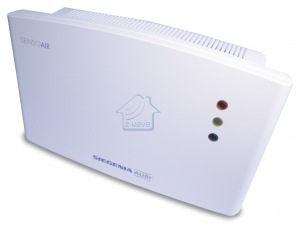
\includegraphics[width=0.24\textwidth]{img/Sensorauswahl/SensoAir.jpeg}
	& 355,81 €
	& Sensoair Z-Wave CO$_2$ Sensor - Table (Tischgerät)
	& CO$_2$; Einsatzmöglichkeit zur Personenerkennung nicht geklärt; wird nur für Überwachung der Luftqualität beworben; mit Fensterkontakt kombinierbar
	\\
	\hline
	\vspace{0cm}\includegraphics[width=0.24\textwidth]{img/Sensorauswahl/Philio.jpeg}
	& 64,13 €
	& Z-Wave 4 in 1 Sensor (Door, Motion, Illumination, Temperature) \newline \textbf{PHI\_PST02-1A}
	& Tür-  Fensterkontakt, Bewegungsmelder, Helligkeit, Temperatur \\
	\hline
	\vspace{0cm}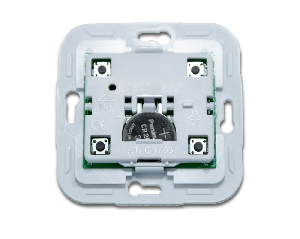
\includegraphics[width=0.24\textwidth]{img/Sensorauswahl/PoppWallController.jpg}
	& 37,01 €
	& Z-Wave.Me Funkwandschalter \newline \textbf{ZMEEWALLC-2}
	& Wandschalter zur Simulation eines Türschlosses oder für einen Abbruchmechanismus einer eingehenden Aktion\\
	\hline
	\vspace{0cm}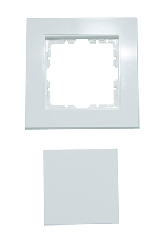
\includegraphics[width=0.24\textwidth]{img/Sensorauswahl/PoppFrame.jpg}
	& 7,98 €
	& Rahmen + Einzelwippe System 55 \newline \textbf{ZME\_SW7}
	& Rahmen für Schalter\\
	\hline
	\vspace{0cm}
\includegraphics[width=0.24\textwidth]{img/Sensorauswahl/FibaroWallPlug.jpg}
	& 63,89 €
	& Zwischenstecker Schalter Typ F (Schuko) \newline \textbf{FIBEFGWPF-102}
	& Aktor zur Demonstration, außerdem Sensor Stromverbrauch \\
	\hline
	\caption{Übersicht bestellter Sensoren}
\end{longtabu}

%%%%%%%%%%%%%%%%%%%%%%%%%%%%%%%%%%%%%%%%%%%%%%%%%%%%%%%%%%%%%%%%%%%%%%%%%%%%%%%%
\section{Sensorevaluation}
Dieser Abschnitt soll die ausgewählten Sensoren (\prettyref{sec:sensorAuswahl}) im Detail beschreiben und charakterisieren. Dabei wird analysiert, welche Funktionen von den Sensoren wie erwartet erfüllt werden, bzw. in welchen Bereichen die Geräte nicht wie angenommen arbeiten.

Die Geräte stellen zahlreiche Konfigurationsparameter bereit, über diese kann die Arbeitsweise der Sensoren an die Anforderungen angepasst werden. Diese Parameter zu überprüfen, deren Änderung auf die Arbeitsweise zu untersuchen und geeignete Konfigurationen in Hinblick auf die Szenarien zu finden, ist Ziel dieses Abschnitts.

Dabei soll festgestellt werden, ob grundsätzliche technische Probleme auftreten und wie sich diese bestenfalls lösen oder zumindest so weit einschränken lassen, dass sie der geplanten Verwendung der Geräte nicht im Wege stehen.

%\begin{itemize}
%	\item Ergebnisse der Sensorevaluation (je Sensor)
%	\item Was funktioniert wie erwartet/was nicht?
%	\item Welche technischen Probleme, lassen sich diese einschränken?
%	\item Sind Probleme auf Hardware/Software zurückzuführen?
%\end{itemize}

\subsection{Fibaro Multisensor}
\emph{(von Philip Laube)}

\subsubsection{Allgemein}

\begin{description}
	\item[Energieversorgung] CR123A Batterie, 3,6 VDC
	\item[Empfohlene Installationshöhe] 2,4 m
	\item[Temperaturreichweite] -20 °C bis 100 °C
	\item[Temperaturgenauigkeit] 0,5 °C bei 0 °C bis 40 °C
	\item[Lichtintensitätsreichweite] 0 – 32000 LUX
	\item[Reichweite des Z-Wave Funk] bis zu 50 m außerhalb von Gebäuden, bis zu 30 m innerhalb von Gebäuden
	\item[Reichweite des Bewegungssensors] 7 m
\end{description}

\begin{figure}[h!]
	\centering
	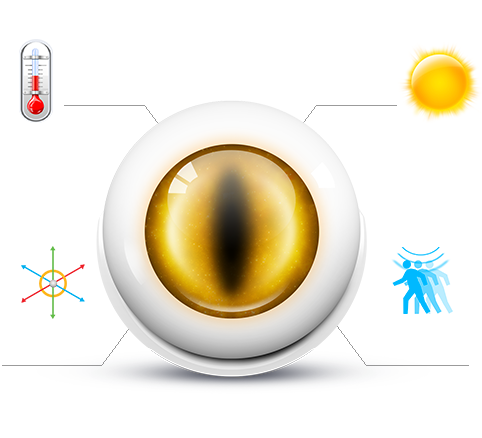
\includegraphics[scale=0.4]{img/Sensorevaluation/FibaroMulti.png}
	\caption{Fibaro Multisensor}
	\label{fig:sensorenFibaroMulti}
\end{figure}

Dieses Gerät ist vielseitig einsetzbar, da eine Vielzahl von Sensoren zur Verfügung stehen. Die Bewegungssensoren sollen dazu verwendet werden eine Person beim Durchgehen eines Türdurchganges zu beobachten.
Neben dem Bewegungssensor beinhaltet der Fibaro Multisensor ein Thermometer, einen Lichtsensor sowie einen Erschütterungssensor.
Der Erschütterungssensor wird standardmäßig als Diebstahlschutz verwendet um zusätzliche Ereignisse auszulösen.

\begin{figure}[h!]
	\centering
	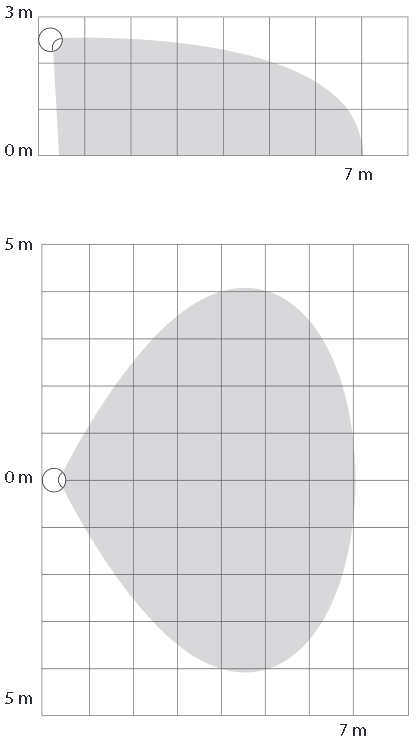
\includegraphics[scale=0.4]{img/Sensorevaluation/FibaroMultiRange.png}
	\caption{Reichweite des Bewegungssensors}
	\label{fig:sensorenFibaroMultiRange}
\end{figure}
 
\begin{figure}[h!]
	\centering
	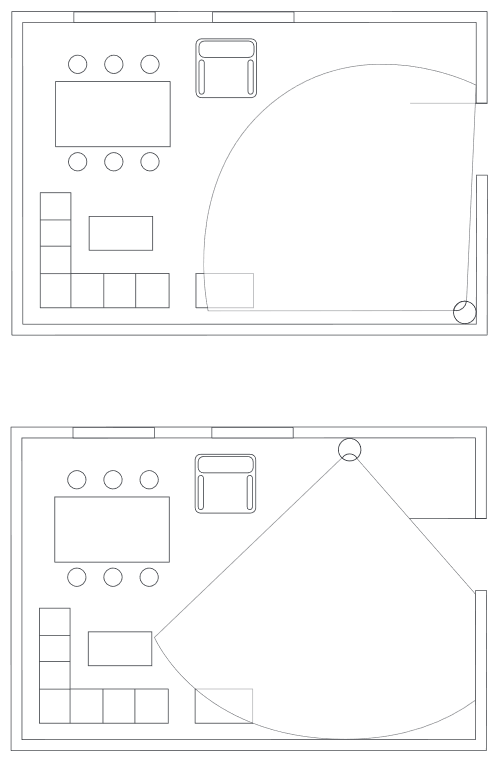
\includegraphics[scale=0.4]{img/Sensorevaluation/FibaroMultiExamples.png}
	\caption{Generelle Installationspunkte zum Beobachtung eines Raumes}
	\label{fig:sensorenFibaroMultiExamples}
\end{figure}

\subsubsection{Praxistest – Türdurchgang}
Für die Konfiguration der Geräte müssen folgende Anpassungen vorgenommen werden:
\begin{description}
	\item [Parameter 1] = 8
	\item [Parameter 2] = 0
	\item [Parameter 6] = 1 (Sekunden)
	
\end{description}

Das hat dann zur Folge, dass jede Sekunde ein Event geworfen wird. Mit diesen Parametern wird zudem jede kleinste Bewegung eines Menschen, die für eine solche Funktion notwendig ist, erkannt. Nun werden pro Raum ein Sensor vor die Tür mit Sicht zur Tür befestigt. Diese werden dann später von einem Modul der diesen Raumdurchgang implementiert benutzt.

\subsubsection{Parameterübersicht}
\begin{description}
	\item [Parameter 1] Wird benutzt um die Sensitivität des Sensors einzustellen und ist ein Wert zwischen 8 und 255 wobei ein kleinerer Wert eine höhere Sensitivität zur Folge hat.
	\item [Parameter 2] Gibt einen Wert an, um den Bewegungssensor für gewisse Zeit nach dem Erkennen von Bewegung blind zu stellen. Dabei ist der Wertebereich hier zwischen 0 – 15, wobei eine Einheit einer halben Sekunde entspricht. So entspricht ein Wert von 0 0,5 Sekunden während ein Wert von 15 8 Sekunden entspricht.
	\item [Parameter 6] Anzahl der Sekunden, nach denen der Sensor ein "`Off-Event"' an den Hauptcontroller (hier Z-Way) sendet, der Sensor wechselt dann in den inaktiven Zustand. Erkannte Bewegungen innerhalb dieses Zeitfensters verlängern das Intervall entsprechend. Um dem entgegenzuwirken kann Parameter 2 weiter angepasst werden.
\end{description}

Mit diesen eingestellten Parametern kann nun bei einem Türdurchgang mit zwei solcher Bewegungssensoren eine Person zuverlässig erkannt werden. Ein Personenzähler speichert dabei die erkannten Werte dauerhaft. 

\begin{description}
	\item [Parameter 8] Gibt nur an zu welcher Tageszeit der Sensor aktiv sein soll. Bei dem Wert 0 ist er den ganzen Tag aktiv, bei dem Wert 1 nur am Tag und bei einem Wert von 2 nur bei Nacht. Hinzuzufügen ist hier, dass die Bestimmung ob Tag oder Nacht ist, durch den internen Lichtsensor realisiert wird. Dieser Wert kann unter dem Parameter 9 eingestellt werden.
	\item [Parameter 20] Die Sensitivität des Erschütterungssensors (Wertebereich 0 – 122 = 0,08 –  2 g = Wert * 0,016 g).
	\item [Parameter 22] Alle wie viele Sekunden wird der Sensor zurückgesetzt und ein neuer Erschütterungswert kann gesendet werden.
	\item [Parameter 26] Der Alarm kann hiermit über einen Broadcast an alle Geräte in der Reichweite gesendet werden, sofern diese einen solchen Broadcast empfangen können.
	\item [Parameter 40] Die minimale Änderung des einfallenden Lichts in Lux um den aktuellen Lux Wert zu senden.
	\item [Parameter 42] Alle wie viele Sekunden soll der Lux Wert gesendet werden, unabhängig von der Änderung des einfallenden Lichts.
	\item [Parameter 60] Die minimale Änderungen der Temperatur bis der aktuelle Wert gesendet wird.
	\item [Parameter 62] Alle wie viele Sekunden wird die Temperatur gemessen.
	\item [Parameter 64] Alle wie viele Sekunden soll der Temperatur-Wert gesendet werden, unabhängig von der Änderung der Temperatur.
	\item [Parameter 66] Anpassung der erkannten Temperatur zur Kalibrierung des Geräts.
	\item [Parameter 80+] Alle Einstellungen für die integrierte LED des Sensors.
\end{description}

\subsubsection{Weitere Funktionalitäten}
Mit dem Parameter 24 = 4 und einer eingestellten minimalen Vibration in Parameter 20 sowie einem Intervall in Parameter 22 in Sekunden kann ein Seismograph eingestellt werden. Dabei wird ab dem Erreichen des Minimalwertes intervallmäßig der erkannte Erschütterungswert gesendet solang die Erschütterung über dem Minimalwert anhält.
%TODO Quellen ergänzen
%Weitere Einstellungen, sowie alle konkreten Wertebereiche sind in der Anleitung Motion-Sensor_EN_5.3.14.pdf zu finden.

%http://www.fibarouk.co.uk/counting-people-using-two-motion-sensors/
%http://www.fibaro.com/manuals/en/Motion-Sensor/Motion-Sensor_EN_5.3.14.pdf
%http://www.fibaro.com/de/the-fibaro-system/motion-sensor
%http://www.fibaro.com/sites/all/themes/fibaro/images/motion-sensor/en/motion_sensor_02.png


\subsection{Fibaro Wall Plug (FGWPx-102) – Zwischenstecker}
\label{subsec:fibaroWallPlug}

\emph{(von Patrick Hecker)}
\subsubsection{Funktionalität}
\begin{itemize}
	\item Z-Wave kompatibler Zwischenstecker in Form eines Steckdosenadapters
	\item Steuerung elektrischer Geräte (max. 2,5 kW)
	\item Messung von Wirkleistung und Stromverbrauch
	\item Anzeige über Schaltzustand und Stromverbrauch über Mehrfarben-LED-Ring
	\item Steuerung am Gerät über Taste
\end{itemize}

\begin{figure}[h!]
	\centering
	
\includegraphics[width=0.6\textwidth]{img/Sensorevaluation/FibaroWallPlug.jpg}
	\caption{Fibaro Wall Plug}
	\label{fig:sensorenFibaroWallPlug}
\end{figure}

\subsubsection{Z-Way Elemente}
\begin{itemize}
	\item Fibaro Wall Plug
	\begin{itemize}
		\item Binary Switch
		\item Steuerung des Schaltzustandes
	\end{itemize}
	\item Meter Electric
	\begin{itemize}
		\item Sensor Multilevel
		\item Stromverbrauch in kW
	\end{itemize}
	\item Sensor Power
	\begin{itemize}
		\item Sensor Multilevel
		\item Wirkleistung in W
	\end{itemize}
\end{itemize}

\subsubsection{Konfiguration}

\paragraph{Immer An - Funktion}
\begin{itemize}
	\item Parameter 1:
	\begin{description}
		\item [0] aktiviert,
		\item [1] deaktiviert
	\end{description}
\end{itemize}

\paragraph{Der Zwischenstecker kann auf Z-Wave Netzwerk Alarm reagieren}
\begin{description}
	\item [Parameter 34:] Welcher Alarm soll Reaktion auslösen?
	\begin{description}
		\item [1] genereller Alarm
		\item [2] Rauchalarm
		\item [4] CO Alarm
		\item [8] CO$_2$ Alarm
		\item [16] Temperaturalarm
		\item [32] Überflutungsalarm
		\item [63] auf jeden Alarm reagieren
	\end{description}
	\item [Parameter 35:] Reaktion auf Alarm
	\begin{description}
		\item [0] keine Reaktion,
		\item [1] Schaltzustand ein,
		\item [2] Schaltzustand aus, zyklischer Wechsel (an/aus) jede Sekunde	
	\end{description}
	\item [Parameter 39:] Dauer der Reaktion
	\begin{itemize}
		\item 1 – 65536 Sekunden
	\end{itemize}
\end{description}

\paragraph{Aussenden verschiedener Reports}
\begin{description}
	\item [Parameter 40 - 45] nur bei Änderung des Stromverbrauchs
	\item [Parameter 47] periodisch, ohne Berücksichtigung des Stromverbrauchs
	\begin{description}
		\item [Parameter 40:] Sofortiger Report über Stromverbrauch (W)
		\begin{itemize}
			\item 1 – 100 \% (Änderung des Stromverbrauchs)
		\end{itemize}
		\item [Parameter 42:] Standardmäßiges Aussenden von Reports über den Stromverbrauch
		\begin{itemize}
			\item 1 – 100 \% (Änderung des Stromverbrauchs)
		\end{itemize}
		\item [Parameter 43:] Zeitintervall zum Senden eines Reports über den Stromverbrauch
		\begin{itemize}
			\item 1 – 254 Sekunden (bezieht sich auf Parameter 42)
		\end{itemize}
		\item [Parameter 45:] Änderung in der Stromaufnahme durch gesteuerte Geräte (kWh)
		\begin{itemize}
			\item 1 – 254 (0,01 – 2,54 kWh)
		\end{itemize}
		\item [Parameter 47:] Zeitintervall zwischen den Reports über die momentane Wirkleistung und den Stromverbrauch
		\begin{itemize}
			\item 1 – 65534 Sekunden
			\item Erklärung: Report im Zeitintervall, ohne Änderung im Verbrauch!
		\end{itemize}
		\item [Parameter 49:] Messen des Eigenstromverbrauchs des Wall Plug Moduls
		\begin{description}
			\item [0] keine Einbeziehung des Eigenstromverbrauchs
			\item [1] inklusive Eigenstromverbrauch
		\end{description}
	\end{description}
\end{description}

\paragraph{Einstellungen zu Assoziationsgruppe 2}
\begin{description}
	\item [Parameter 50:] Unterer Leistungsschwellwert
	\item [Parameter 51:] Oberer Leistungsschwellwert
	\item [Parameter 52:] Konfiguration des Verhaltens beim Überschreiten der festgelegten Leistungsschwellwerte (z.B. das Aus- oder Einschalten aller assoziierten Geräte beim unterschreiten des unteren Leistungsschwellwerts (Parameter 50))
\end{description}

\paragraph{Farbeinstellungen}
\begin{description}
	\item[Parameter 60:] Leistungsschwellwert für violettes Blinken
	\begin{itemize}
		\item 1000 – 32000 (100 – 3200 W)
	\end{itemize}
	\item [Parameter 61:] LED-Ring-Farbe im Einschaltzustand
	\item [Parameter 62:] LED-Ring-Farbe im Ausschaltzustand
	\item [Parameter 63:] LED-Ring-Farbe bei Z-Wave-Alarmmeldung
	\item [Parameter 61 - 63:] Farbwerte
	\begin{description}
		\item [1] White
		\item [2] Red
		\item [3] Green
		\item [4] Blue
		\item [5] Yellow
		\item [6] Cyan
		\item [7] Magenta
		\item [8] Farbe aus
	\end{description}
\end{description}
Weitere Informationen (auch technische Details) sind dem Handbuch zu entnehmen (\url{http://www.fibaro.com/manuals/de/FGWPx-101/FGWPx-101-DE-A-v1.00.pdf}).


\subsection{Aoetec Multisensor Sensor}
\emph{(von Alexander Keller)}

\subsubsection{Allgemein}

Im Bereich Smarthome hat man eine riesige Auswahl von verschiedenen Sensoren. Je nach Bedarf bieten die Multisensoren verschiedene Funktionalitäten welche Bewegungen, Raumtemperatur, Licht oder andere registrieren können. Der Aeotec Sensor erfasst 6 verschiedene Messwerte. Die Sensoren messen Raumtemperatur, Lichtstärke, Luftfeuchtigkeit, Bewegung, UV-Sensor und Vibration. Diese Werte überträgt der Multisensor mit einer drahtlosen Kommunikationsschnittstelle names Z-Wave.

In unserem Projekt kommt dieser Sensor zum Einsatz, um das \emph{AlarmModule}, \emph{PersonIdentificationModule} und \emph{TurnOffHazardModule} mithilfe seiner Sensortechnik zu unterstützen.


\subsubsection{Konfigurationsmöglichkeiten}

Nachdem man das Gerät erfolgreich im Z-Way Home Center hinzugefügt hat, besteht die Möglichkeit den Multisensor über die Expert-UI zu konfigurieren.

\begin{figure}[h!]
	\centering
	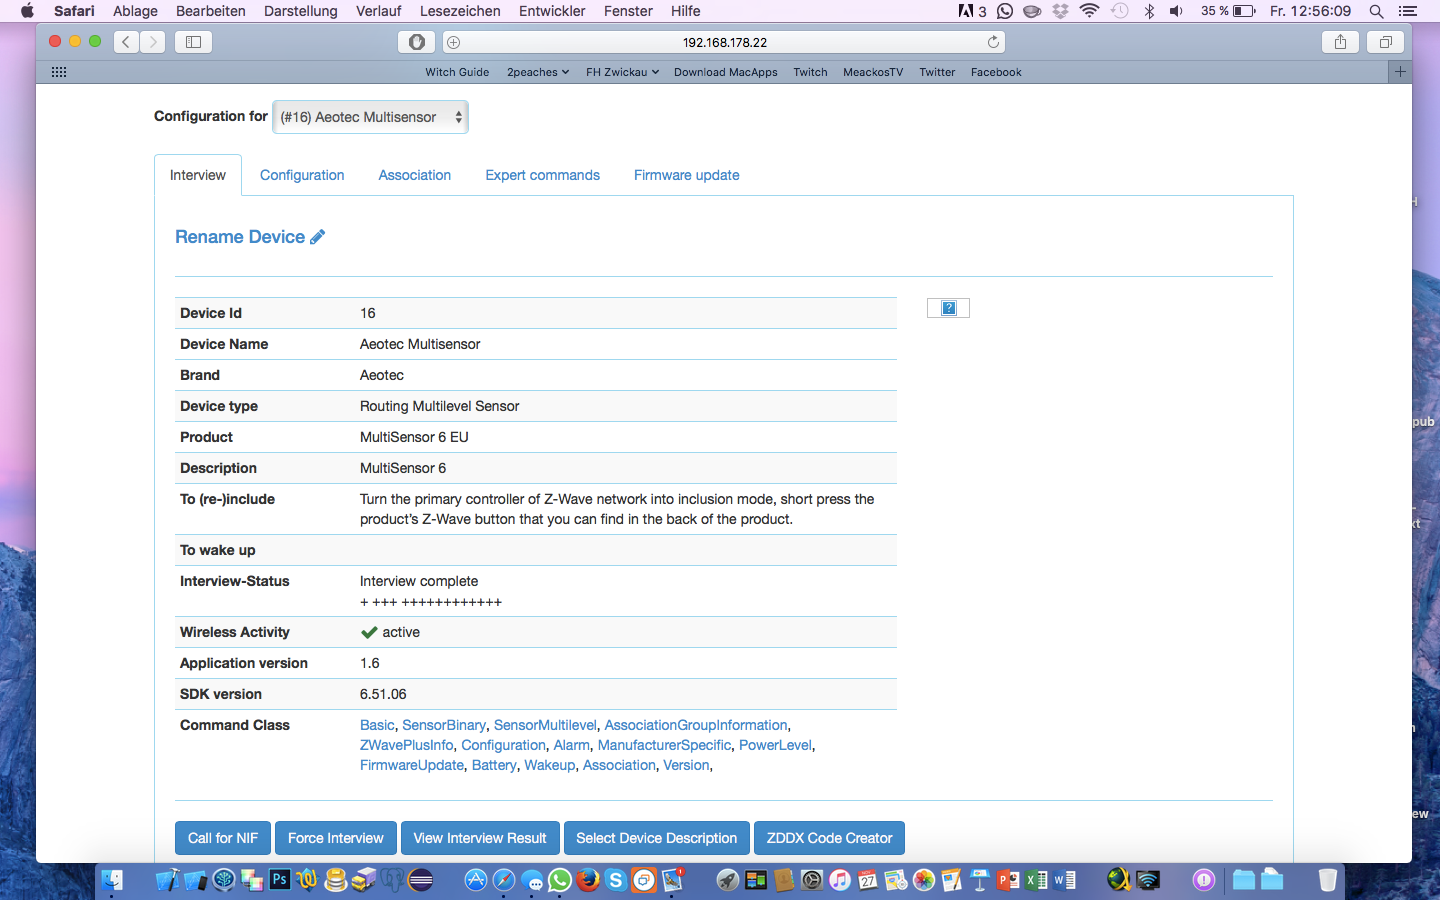
\includegraphics[width=0.9\textwidth]{img/Sensorevaluation/AeoScreenshot.png}
	\caption{Übersichtsseite des Aeotec Multisensor}
	\label{fig:sensorenAeoScreenshot}
\end{figure}

Der Z-Way Server erstellt automatisiert eine Übersichtsseite nachdem der Sensor erfolgreich hinzugefügt wurde. In diesem Reiter besteht die Möglichkeit das Gerät umzubenennen, Netzwerkstatus abzurufen, \gls{sdk} Version.

Im Reiter „Configuration“ findet man alle Einstellungsmöglichkeiten die der Sensor bietet. In der nachfolgenden Tabelle, finden sie alle Konfigurationsoptionen.
\begin{longtabu} to \linewidth {
		>{}X
		>{}X
		>{}X
	}
	
	% ----------- headings -----------
	\hline
	\textbf{Name}							& \textbf{Optionen}		& \textbf{Beschreibung} \\
	\hline
	\endfirsthead
	\hline
	\textbf{Name}							& \textbf{Optionen}		& \textbf{Beschreibung} \\
	\hline
	\endhead
	\hline 
	% ----------- end headings -----------
	% ----------- begin footer -----------
	\multicolumn{3}{r}{{Fortsetzung auf nächster Seite}}  \\ 
	%\hline
	\endfoot
	%\hline
	\endlastfoot
	% ----------- end footer -----------
	Wake Up 10 Minutes when	batteries are inserted	
			& No \newline Yes				
					& Der Sensor "`erwacht"' alle 10 Minuten, wenn Batterien eingelegt sind. \\ 

	\hline 
	On Time									& X Minuten	 		& Wie lang sollen die verschiedenen Sensoren den aktuellen Wert speichern bevor diese aktualisiert werden \\ 
	\hline
	Enable/Disable the function of motion Sensor &
			(0) disable \newline
			(1) enable, the current PIR sensitivity level=1. (minimum level) \newline
			(2) enable, the current PIR sensitivity level = 2. \newline
			(3) enable, the current PIR sensitivity level=3. \newline
			(4) enable, the current PIR sensitivity level=4. \newline
			(5) \uline{enable, the current PIR sensitivity level=5. (maximum level)} \newline &
					Es besteht die Möglichkeit den Bewegungssensor zu deaktivieren \& die Intensität einzustellen \\
	\hline
	Motion Detection &
			(1) \uline{Send Basic Set CC.} \newline
			(2) Send Sensor Binary Report CC. &
					Welchen Standard soll der Aeotec Sensor sende, wenn der Bewegungssensor ausgelöst wurde \\
	\hline
	Low Batterie Value &
			X \% &
					Ab welchen prozentualen Wert soll der Sensor bescheid geben, wenn der Batteriestand niedrig ist. \\
	\hline
	Reports for Parameter 41 – 44 &
			(0) \uline{disable} \newline
			(1) enable &
					Diese Funktionalität dient dazu um bestimmte Schwellenwerte in bestimmten Zeitabständen zu an den Z-Way Server zu senden. (Netzwerktraffic) \\
	\hline
	Humidity Automatic Report &
			X Schwellenwert &
					Festlegen eines Schwellenwertes für den Feuchtigkeitssensor \\
	\hline
	Luminance Automatic Report &
			X Luminanz &
					Festlegen eines Schwellenwertes für den Lichtsensor \\
	\hline
	Battery Automatic Report &
			X Prozent &
					Festlegen eines Schwellenwertes für die Batterieänderung \\
	\hline
	Threshold change in ultraviolet to induce an automatic report. &
			X Schwellenwert &
					Festlegen eines Schwellenwertes für Ultra Violettes Licht \\
	\hline
	Low Temperature Alarm Report &
			(0) Disable to send the alarm report of low temperature \newline
			(1) Enable to send the alarm report of low temperature &
				 Bericht wenn die Temperatur unter 15 Grad fällt. \\
	\hline
	Unsolicitate reports interval for timing groups 1 / 2 / 3 &
			X Sekunden &
					Alle X Sekunden sendet der Motion Sensor einen Bericht. \\
	\hline
	Lock Configuration &
			(0) Disable all configuration parameters to be locked.\newline
			(1) Enable all configuration parameters to be locked. &
					Alle Änderungen von Parametern werden gespeichert. \\
	\hline
	Reset to default factory setting &
			(1) Resets all configuration parameters to default setting. \newline
			(1431655765) Reset the product to default factory setting and be excluded from the Z-wave network. &
					Hier besteht die Möglichkeit den Mutlisensor komplett auf Werkseinstellung zurückzusetzen \& ihn anschließend aus dem Z-Way Netzwerk zu entfernen. \\
	\hline
	WakeUp Settings &
			X Sekunden &
					Nach wie vielen Sekunden der Sensor erwachen sollen, wenn keine Aktivität vorhanden war \\
	\hline
		
\caption{Konfiguration des Aeotec-Sensors} \\
\end{longtabu}

\subsubsection{Praxistest}
Um das Gerät ausführlich testen zu können, ist es notwendig als ersten Schritt die Batterien einzulegen. Der Motion Sensor von Aeotec benötigt 4x AAA Batterien, welche mindestens 12 Monate lange halten.
\subsubsection{Motion Sensor}
Die effektive Reichweite des Bewegungssensors ist begrenzt. Anhang der Skizze ist zu erkenne, dass der Radius bei einer Höhe von 3 Metern, maximal 10 Meter beträgt.

\begin{figure}[h!]
	\centering
	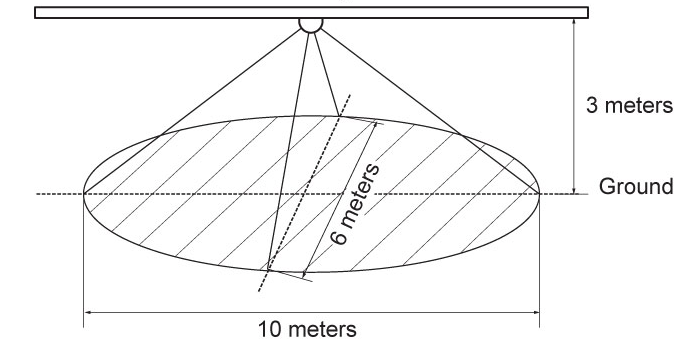
\includegraphics[width=0.9\textwidth]{img/Sensorevaluation/AeoMeter1.png}
	\caption{Bewegungssensor in der Praxis ohne Hindernisse}
	\label{fig:sensorenAeoMeter1}
\end{figure}

Falls eine Wand oder andere Hindernisse im Weg sind muss die Berechnung des Durchmesser, sowie die Reichweite des Bewegungssensors individuell angepasst werden. Im folgenden Beispiel hängt der Sensor von Aeotec nicht an der Decke, sondern ist an einer Wand befestigt.

\begin{figure}[h!]
	\centering
	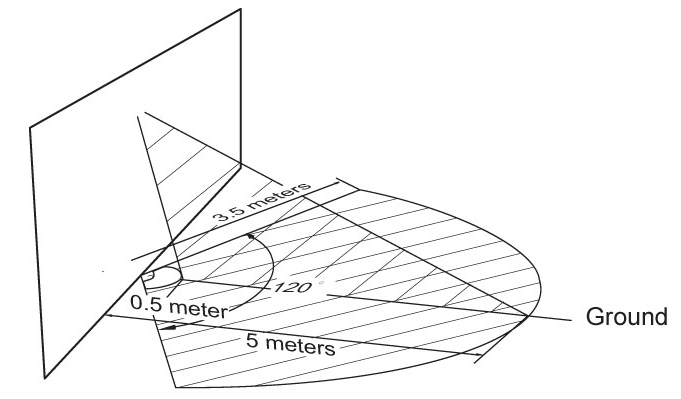
\includegraphics[width=0.9\textwidth]{img/Sensorevaluation/AeoMeter2.png}
	\caption{Bewegungssensor in der Praxis an einer Wand}
	\label{fig:sensorenAeoMeter2}
\end{figure}

\subsubsection{Temperatur}
\begin{figure}[h!]
	\centering
	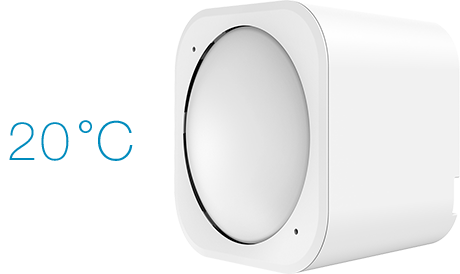
\includegraphics[width=0.5\textwidth]{img/Sensorevaluation/AeoTemp.png}
	\caption{Aoetec Temperatursensor}
	\label{fig:sensorenAeoTemp}
\end{figure}

Der Multisensor der Firma Aeotec bietet die Möglichkeit dem Nutzer die aktuelle Raumtemperatur anzuzeigen. Im Praxistest hat sich gezeigt, dass die Temperatur immer 1 – 3 Grad Celsius zu viel angezeigt hat. Eine Kalibrierung des Sensors ist laut Konfigurationsmöglichkeiten (siehe oben) nicht möglich. Das wiederum heißt, dass der Nutzer seinen Schwellenwert immer um den Mittelwert 2 Grad Celsius anheben sollte.

\subsubsection{Lichtsensor}
\begin{figure}[h!]
	\centering
	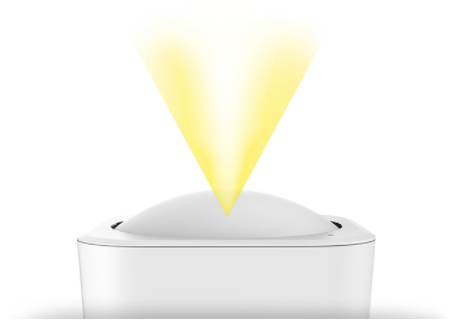
\includegraphics[width=0.5\textwidth]{img/Sensorevaluation/AeoLight.png}
	\caption{Aoetec Lichtsensor}
	\label{fig:sensorenAeoLight}
\end{figure}

In der Praxis erwies sich sich der Lichtsensor für sehr zuverlässig. Der Anwendungsbereich dafür wäre eine automatisierte Rollladensteuerung oder Lampensteuerung.

\subsubsection{Luftfeuchtigkeitssensor}
\begin{figure}[h!]
	\centering
	
\includegraphics[width=0.5\textwidth]{img/Sensorevaluation/AeoHum.png}
	\caption{Aoetec Feuchtigkeitssensor}
	\label{fig:sensorenAeoHum}
\end{figure}

Der Aoetec Sensor besitzt einen Luftfeuchtigkeitssensor mit diesem man die Luftfeuchtigkeit zwischen 0\% und 100\% messen kann. Die praktische Anwendung wäre eine automatisierte Tür- \& Fenstersteuerung, welches ein perfektes Klima im Raum ermöglicht.

\subsubsection{Vibrationssensor}
\begin{figure}[h!]
	\centering
	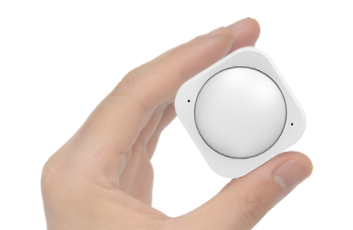
\includegraphics[width=0.5\textwidth]{img/Sensorevaluation/AeoVib.png}
	\caption{Aoetec Vibrationssensor}
	\label{fig:sensorenAeoVib}
\end{figure}

Durch den eingebauten seismischen Sensor überwacht dieser Erschütterungen und Vibrationen. Diese Funktionalität bietet sich bestens um Alarm diesen Vibrationssensor in ein Alarmmodul zu integrieren damit dieser bei ungewöhnlichen Erschütterungen Alarm schlägt.

\subsubsection{UV Sensor}
\begin{figure}[h!]
	\centering
	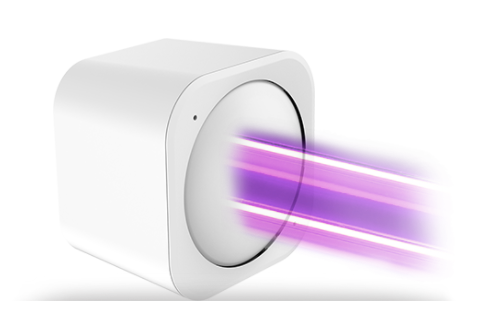
\includegraphics[width=0.5\textwidth]{img/Sensorevaluation/AeoUV.png}
	\caption{Aoetec UV-Sensor}
	\label{fig:sensorenAeoUV}
\end{figure}

Ab einen bestimmten Anteil von ultravioletten Licht ist dieses sehr schädlich für das Auge. Um sich davor zu schützen, sind elektrische Jalousien oder Rollläden notwendig.



\subsection{Philio 4-in-1 Multisensor}
\emph{(von Tobias Weise)}
\subsubsection{Allgemein}
Im Bereich Smart Home existiert eine große Auswahl an unterschiedlichen Sensoren. Je nach Bedarf bietet der Philio 4-in-1 Multisensor verschiedene Funktionalitäten, welche Bewegungen, Tür- und Fenster öffnen bzw. schließen, Licht- oder Temperaturänderungen registrieren können. Der Philio 4-in-1 Multisensor ist somit in der Lage 4 verschiedene Messwerte zu erfassen. Diese Werte überträgt der Multisensor über eine drahtlose Kommunikationsschnittstelle namens Z-Wave an den Z-Way-Server.

Im Rahmen des Projektes kommt dieser Sensor zum Einsatz, um das Öffnen und Schließen der Wohnungstür, sowie Bewegungen innerhalb des Raumes zu registrieren. Dabei findet er hauptsächlich in den Modulen \emph{LockDoorModule}, \emph{PersonCounterModule} und \emph{StandbyModule} Verwendung. Durch die vielseitigen Einstellungsmöglichkeiten der Parameter des Sensors, wird nachfolgend eine Evaluierung der Optionen durchgeführt.

\begin{figure}[h!]
	\centering
	\includegraphics[width=0.4\textwidth]{img/Sensorevaluation/Philio.jpeg}
	\caption{Philio 4-in-1 Multisensor}
	\label{fig:sensorenPhilioMultisensor}
\end{figure}

\subsubsection{Konfigurationsmöglichkeiten}
Nachdem der Sensor erfolgreich in das Z-Wave-Netzwerk hinzugefügt wurde, besteht die Möglichkeit, den Multisensor über die Expert-UI zu konfigurieren.

\begin{figure}[h!]
	\centering
	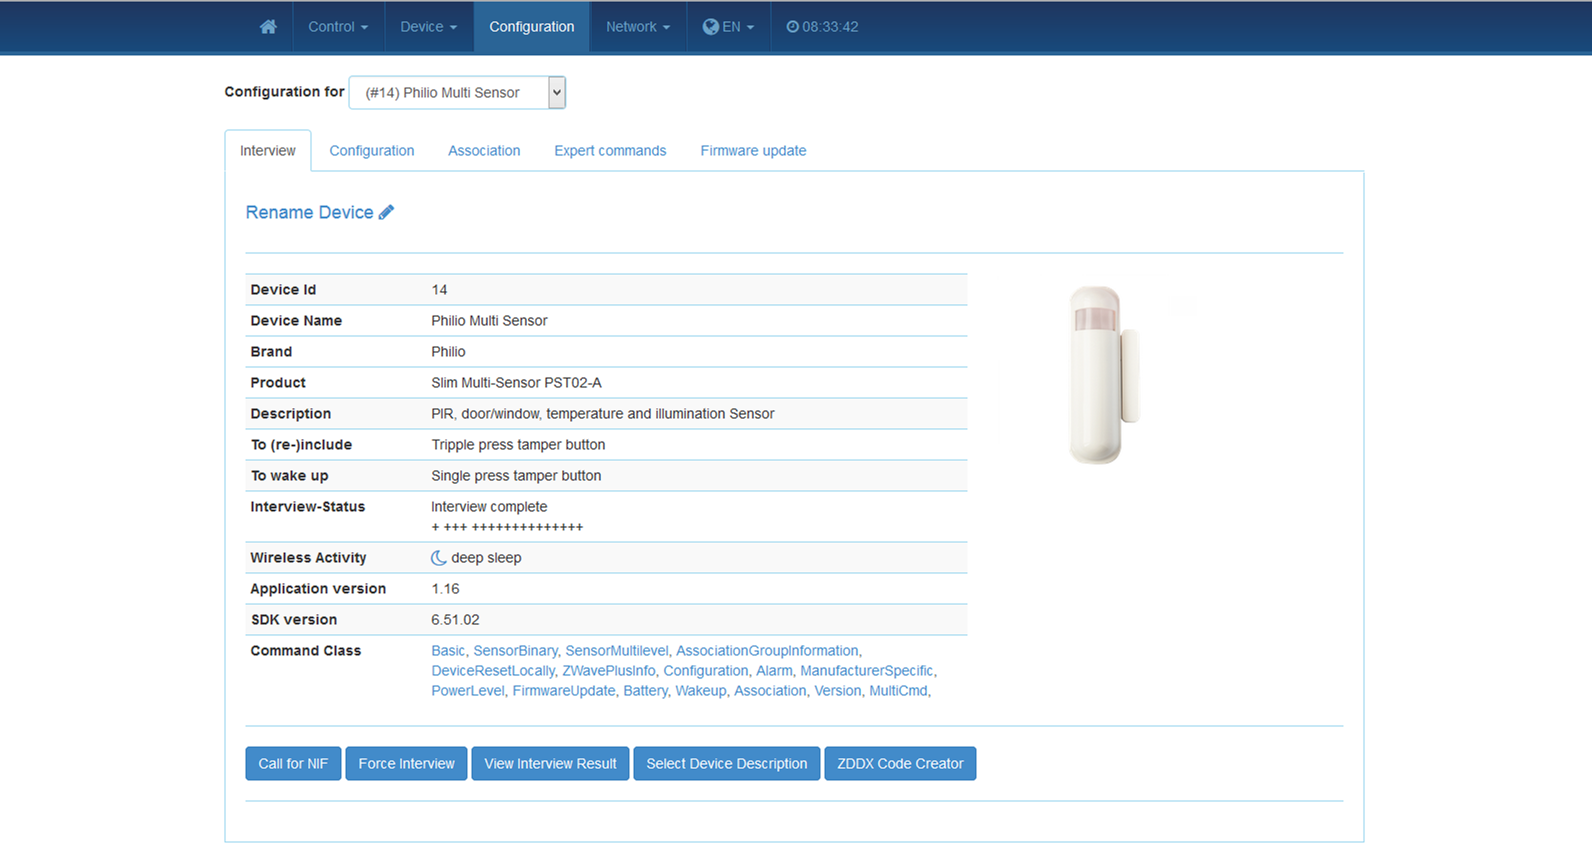
\includegraphics[width=0.9\textwidth]{img/Sensorevaluation/PhilioConf1.png}
	\caption{Übersichtsseite des Philio 4-in-1 Multisensors}
	\label{fig:sensorenPhilioConf1}
\end{figure}

Der Z-Way-Server erstellt automatisiert eine Übersichtsseite, nachdem der Sensor erfolgreich hinzugefügt wurde. In diesem Reiter besteht die Möglichkeit, das Gerät umzubenennen, den Netzwerkstatus abzurufen und die aktuelle Sensor-Version abzufragen. Im Reiter "`Configuration"' finden sich alle Einstellungsmöglichkeiten die der Sensor bietet. Nachfolgend sind die wichtigsten Konfigurationsoptionen in einer Tabelle (\prettyref{tab:PhilioConf}) aufgelistet.


\begin{longtabu} to \linewidth {
		>{\hsize=0.05\hsize}X
		>{\hsize=0.8\hsize}X
		>{\hsize=1.4\hsize}X 
		>{\hsize=1.75\hsize}X
		% sum=4.0\hsize for 4 columns
	}
	% ----------- begin header -----------	
	\hline
	\textbf{Nr}
			& \textbf{Name}
					& \textbf{Beschreibung}
							& \textbf{Werte} \\
	\hline
	\endhead
	% ----------- end header -----------
	
	% ----------- begin footer -----------
	\multicolumn{4}{r}{{Fortsetzung auf nächster Seite}}  \\ 
	\endfoot
	\endlastfoot
	% ----------- end footer -----------
	
	\hline
	2	
			& Grundeinstellung 
					& Setzt den Standardwert, um das Licht einzuschalten.
							& -1 \textrightarrow{ }einschalten \newline 1 – 99 \textrightarrow{ }Dimmerintensität \\
	\hline
	3	
			& Sensitivität des Bewegungsmelders
					& Festlegen der Bewegungserkennungsintensität.
							& 0 \textrightarrow{ }keine Bewegungserkennung \newline
							1 – 99 \textrightarrow{ }1 ist niedrigste Sensitivität, 99 die höchste \\
	\hline
	4	
			& Lichtschwellwert 
					& Festlegen des Beleuchtungsschwellwertes, um das Licht einzuschalten. Wenn das Event auslöst und die Umgebung dunkler ist, als der Schwellwert, geht das Licht an. 
							& 1 – 99 \textrightarrow{ }1 ist dunkel, 99 ist hellster Wert \newline
							100 \textrightarrow{ }Lichterkennung deaktiviert \newline
							0 \textrightarrow{ }Lichterkennung deaktiviert und das Licht wird nie angeschaltet \\
	\hline
	5	
			& Betriebsmodus 
					& Bit 0 und Bit 1 werden freigeschaltet, sobald der DID-Schalter auf Programmmodus umgeschaltet wurde.
							& (Bit) 0 \textrightarrow{ }Sicherheitsmodus \newline
							(Bit) 1 \textrightarrow{ }Testmodus \newline
							(Bit) 2 \textrightarrow{ }Fenster-/Türsensor deaktiviert \newline
							(Bit) 3 \textrightarrow{ }0 für Fahrenheit, 1 für Celsius \newline
							(Bit) 4 \textrightarrow{ }deaktiviere Lichtwertübergabe bei Auslösen des Events \newline
							(Bit) 5 \textrightarrow{ }deaktiviere Temperaturwertübergabe bei Auslösen des Events
							 \\
	\hline
	6	
			& Multisensor Funktionsschalter
					& Setzt den Standardwert, um das Licht einzuschalten. \newline
							& (Bit) 0 \textrightarrow{ }deaktiviere integrierte Beleuchtung \newline
							(Bit) 1 \textrightarrow{ }deaktiviere integrierte Bewegungsmelder-Beleuchtung \newline
							(Bit) 2 \textrightarrow{ }deaktiviere Bewegungsmelder \newline
							(Bit) 3 \textrightarrow{ }wenn Bit 2 0 ist (aktiviert), ist das Gerät dann im selben Raum installiert? 0 = gleicher Raum (Standard), 1 = anderer Raum \newline
							(Bit) 4 \textrightarrow{ }deaktiviere die Verzögerung von 5 Sekunden beim Licht ausschalten, wenn Tür/Fenster geschlossen wurden \newline
							(Bit) 5 \textrightarrow{ }deaktiviere automatisches Licht ausschalten, nachdem Fenster/Tür geöffnet wurden und das Licht anging (keine Verwendung, wenn Bit 2 = 0) \newline
							(Bit) 6 \textrightarrow{ }Aktiviere die Temperaturaufzeichnung. Temperaturreport alle 64 Sekunden, wenn Veränderung von 3 Grad Fahrenheit und Überschreitung von 140 Grad Fahrenheit \\
	\hline
	8	
			& Bewegungsmelder, erneute Entdeckungszeit
					& Setzen der nächsten Entdeckungszeit, wenn ein Objekt entdeckt wurde und sich das Gerät im Sicherheitsmodus befindet.
							& 3 – 127 \textrightarrow{ }eingegebener Wert mal 8 Sekunden entspricht dem Zeitwert. \newline
							Minimale Zeit beträgt 24 Sekunden. \\
	\hline
	9	
			& Abschaltlichtzeit
					& Setzen der Verzögerungszeit, um das Licht wieder auszuschalten, wenn der Bewegungsmelder nicht ausgelöst hat und nachdem das Licht angeschaltet wurde.
							& 4 – 127 \textrightarrow{ }Eingegebener Wert mal 8 Sekunden entspricht dem Zeitwert. \newline Minimale Zeit beträgt 32 Sekunden. \\
	\hline
	10	
			& Auto-Reportzeit der Batterielebensdauer
					& Intervallzeit für automatische Meldung über die Batterierestkapazität
							& 1 – 127 \textrightarrow{ }Eingegebener Wert mal 30 Minuten entspricht dem Zeitwert. \newline Minimale Zeit beträgt 30 Minuten. \\
	\hline
	11	
			& Auto-Reportzeit  des Fenster/Tür Status
					& Intervallzeit für automatische Meldung des Fenster/Tür Status
							& 1 – 127 \textrightarrow{ }Eingegebener Wert mal 30 Minuten entspricht dem Zeitwert. \newline Minimale Zeit beträgt 30 Minuten. \\
	\hline
	12	
			& Auto-Reportzeit der Beleuchtung
					& Intervallzeit für automatische Meldung des Beleuchtungsstatus
							& 1 – 127 \textrightarrow{ }Eingegebener Wert mal 30 Minuten entspricht dem Zeitwert. \newline Minimale Zeit beträgt 30 Minuten. \\
	\hline
	13	
			& Auto-Reportzeit der Temperatur
					& Intervallzeit für automatische Meldung der Temperatur
							& 1 – 127 \textrightarrow{ }Eingegebener Wert mal 30 Minuten entspricht dem Zeitwert. \newline Minimale Zeit beträgt 30 Minuten. \\
	\hline
\caption{Konfiguration des Philio Multisensor}
\label{tab:PhilioConf}
\end{longtabu}

\subsubsection{Praxistest}
Um das Gerät in das Netzwerk einbinden zu können, ist es für die erste Konfiguration nur notwendig, den Stromkreislauf mit der Batterie zu verbinden und schon verbindet sich das Gerät innerhalb von 5 Sekunden automatisch mit dem Z-Wave-Netzwerk, wenn sich der Controller im "`Inclusion Mode"' befindet. Zu einem späteren Zeitpunkt ist eine Integration in das Netzwerk möglich, indem der Manipulationsschutzschalter auf der Rückseite drei Mal gedrückt wird. Ein einmaliges Drücken des erwähnten Schalters, hat ein "´Wake-up"' zur Folge.

In manchen Fällen besteht nach Recherche allerdings die Möglichkeit, dass nach dem Inkludieren keine Funktion angezeigt wird. Um dem Abhilfe zu schaffen, wurde die nachfolgende Anleitung erstellt.

Z-Wave verfügt über die Möglichkeit, Geräte als "`secure"' in das Z-Wave-Netzwerk zu inkludieren. Dabei erfolgt die Kommunikation zwischen dem Sensor und dem Gateway verschlüsselt. Allerdings ist es in diesem Falle möglich, dass der Philio-Multisensor keine Zustandsänderungen an das Gateway sendet. In diesem Fall muss die Experten-Oberfläche des Z-Way-Servers geöffnet werden. (\prettyref{fig:sensorenPhilioConf2}).

\begin{figure}[h!]
	\centering
	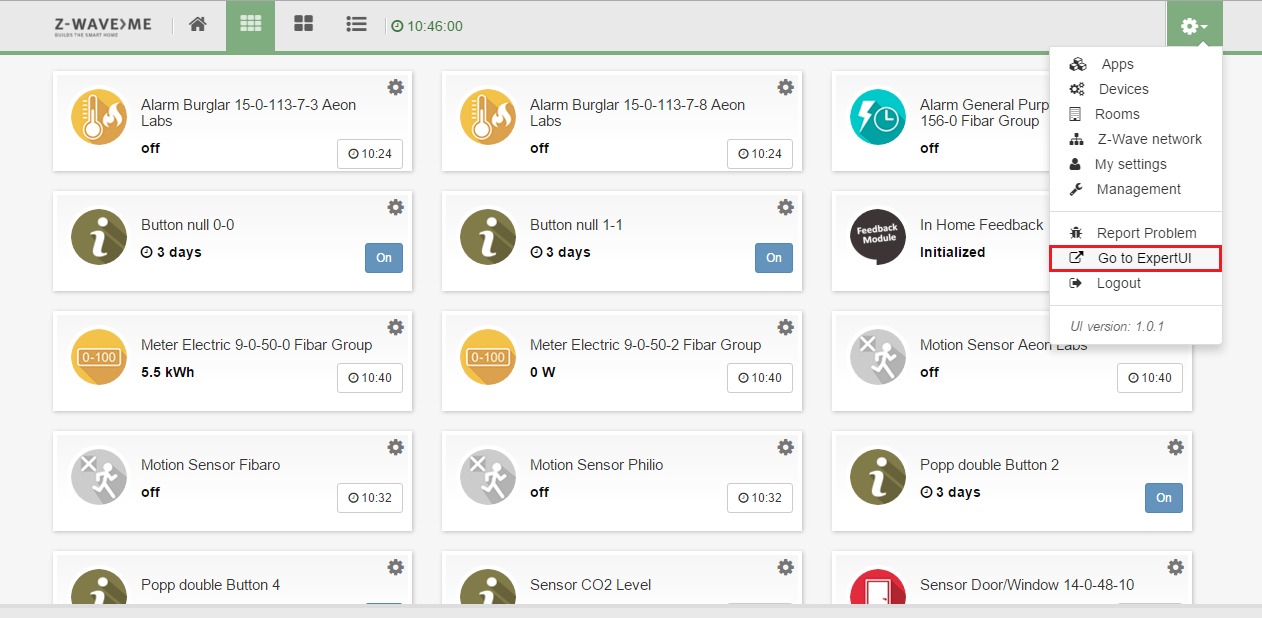
\includegraphics[width=0.9\textwidth]{img/Sensorevaluation/PhilioConf2.png}
	\caption{Oberfläche des Z-Way-Servers}
	\label{fig:sensorenPhilioConf2}
\end{figure}

Anschließend sind die Netzwerkeinstellungen zu öffnen, auf der Experten-Oberfläche  unter "`Network"' und "`Control"' (\prettyref{fig:sensorenPhilioConf3}).

\begin{figure}[h!]
	\centering
	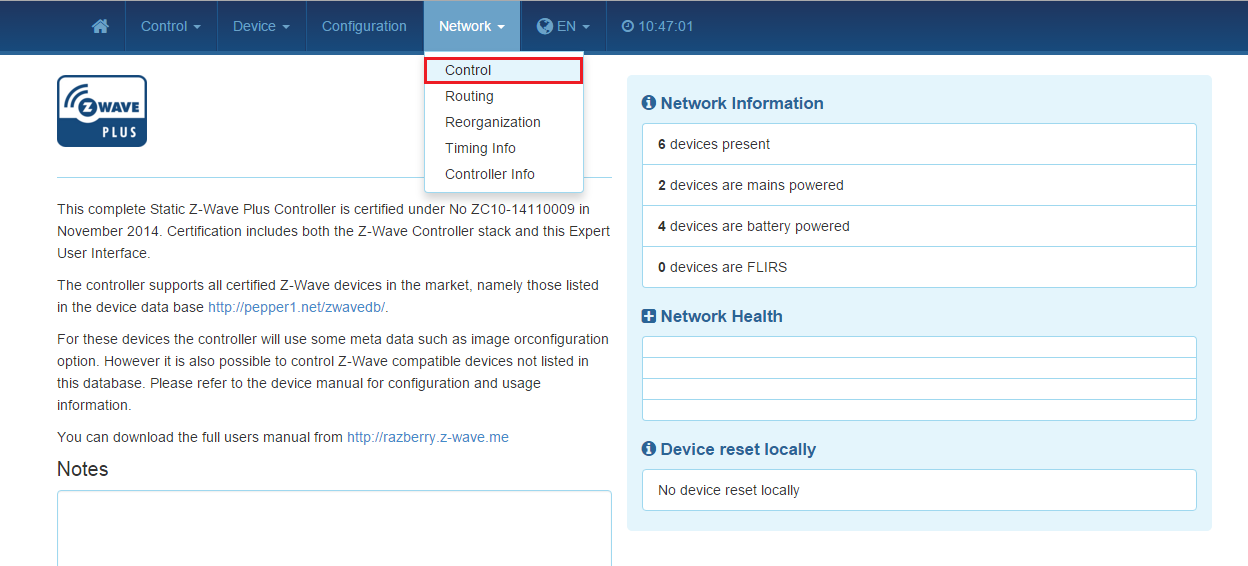
\includegraphics[width=0.9\textwidth]{img/Sensorevaluation/PhilioConf3.png}
	\caption{Experten-Oberfläche}
	\label{fig:sensorenPhilioConf3}
\end{figure}

An dieser Stelle besteht die Möglichkeit, die Art der Inklusion von "`secure"' auf "`unsecure"' zu ändern (1.). Anschließend muss der "`Start Inclusion"'-Button gedrückt werden (2.), um das Inkludieren zu beginnen (\prettyref{fig:sensorenPhilioConf4}). 

\begin{figure}[h!]
	\centering
	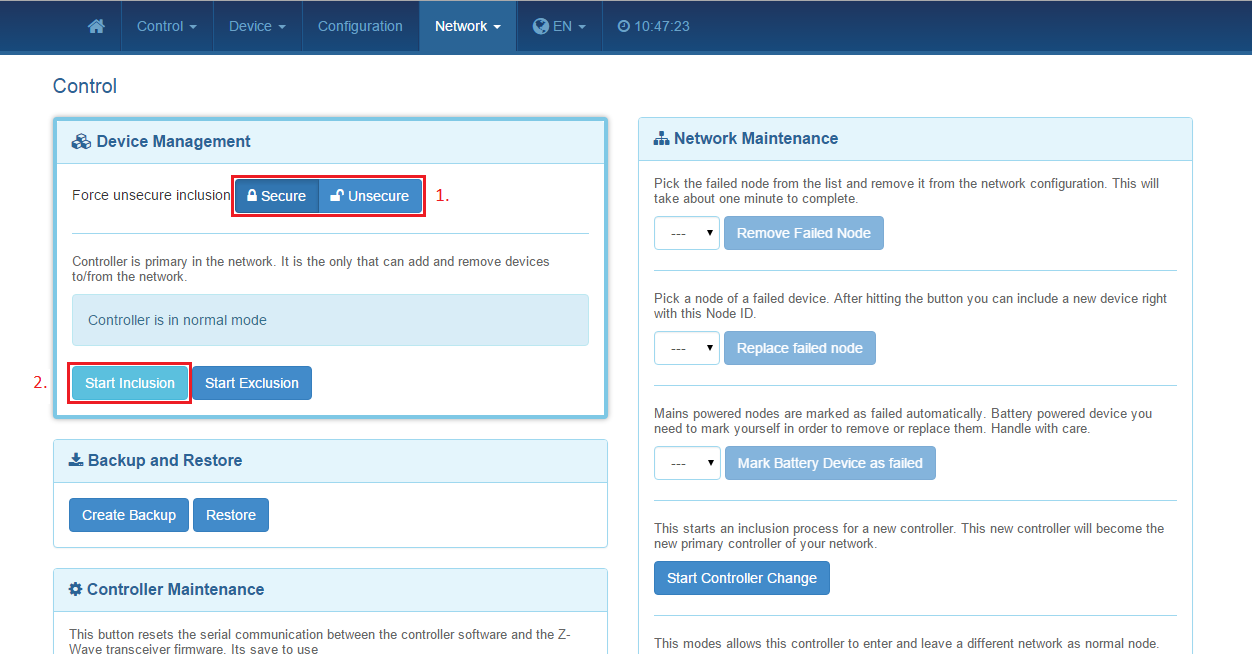
\includegraphics[width=0.9\textwidth]{img/Sensorevaluation/PhilioConf4.png}
	\caption{Auswahl des Inkludiermodus}
	\label{fig:sensorenPhilioConf4}
\end{figure}

Wenn nun die kleine Schalter-Lasche des Sensors dreimal hintereinander (innerhalb von 1,5 Sekunden) betätigt wird, sollte der Multisensor erfolgreich in das Z-Way-Netzwerk integriert worden sein. Auf der Smart Home Benutzeroberfläche werden die Elemente automatisch generiert, welche die Funktionen des Philio-Multisensors darstellen (\prettyref{fig:sensorenPhilioElements}).

\begin{figure}[h!]
	\centering
	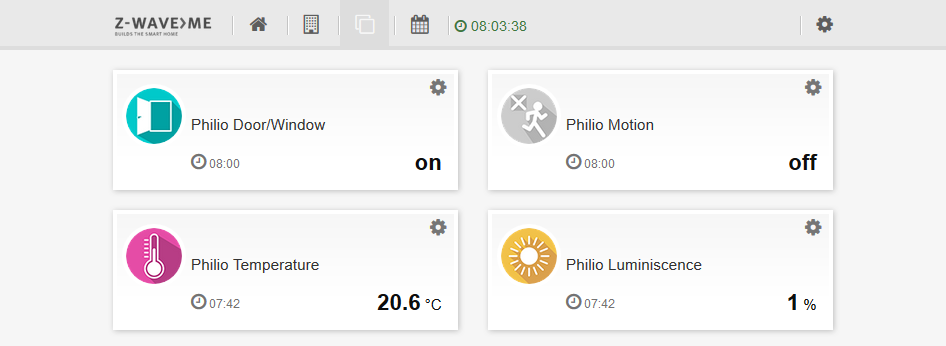
\includegraphics[width=0.9\textwidth]{img/Sensorevaluation/PhilioElements.png}
	\caption{Elemente des Philio Multisensors}
	\label{fig:sensorenPhilioElements}
\end{figure}

\subsection{Sensoair Z-Wave CO$_2$ Sensor (Tischgerät)}

\subsubsection{Beschreibung}
Der Sensor misst die CO$_2$-Konzentration in der Luft in \gls{ppm}. Um die CO$_2$-Konzentration in geschlossenen Räumen erkennen zu können, nutzt die Einheit zwei Sensoren. Der gemessene Werte wird auch über die drei LEDs am Gehäuse symbolisiert. Dabei besitzt der Sensor sieben \gls{ppm}-Warnstufen, welche mithilfe der drei LEDs darstellt werden (\prettyref{fig:sensorenSensoair}).

\begin{figure}[h!]
	\centering
	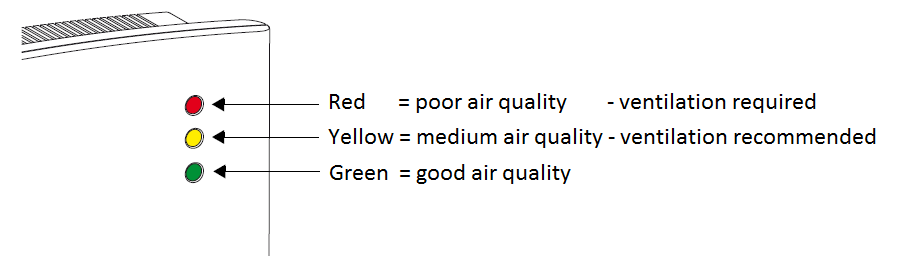
\includegraphics[width=0.9\textwidth]{img/Sensorevaluation/Sensoair.png}
	\caption{Statusanzeigen des Sensoair CO$_2$-Sensors}
	\label{fig:sensorenSensoair}
\end{figure}


\begin{longtabu} to \textwidth{
		>{\hsize=1.0\hsize}X 
		>{\hsize=1.0\hsize}X
	}
	\hline
	\textbf{ppm-Wert (obere Grenze)}	& \textbf{LED-Belegung} \\
	\hline
	\endhead
	% ----------- begin footer -----------
	\multicolumn{2}{r}{{Fortsetzung auf nächster Seite}}  \\ 
	\endfoot
	\endlastfoot
	% ----------- end footer -----------
	350									& grün \\ 
	\hline
	600									& grün und gelb \\
	\hline
	800									& gelb \\
	\hline
	1000								& gelb und rot \\
	\hline
	1500								& rot \\
	\hline
	2000								& einmal langes rotes Blinken \\
	\hline
	2500								& zweimal kurzes rotes Blinken \\
	\hline
	\caption{Visuelle Darstellung von CO$_2$-Messwerten.}
\end{longtabu}

\subsubsection{Besonderheiten bei der Installation}
Der Sensor kann sowohl mit 230 Volt Wechselspannung als auch 24 Volt Gleichspannung betrieben werden, dazu müssen zwei Anschlusskabel ummontiert werden.

Außerdem schreibt die Anleitung einige Bedingungen vor, unter welchen der Sensor genutzt werden soll. Der Sensor ist nur in geschlossenen, trockenen und staubfreien Räumen zu verwenden. Die Verwendung des Sensors ist auf einen Temperaturbereich von 5 – 40 °C beschränkt. Das Gerät ist nicht als Gaswarngerät geeignet und muss von Lösungsmitteln ferngehalten werden, da es zum Beispiel durch Silikondämpfe zu Fehlfunktionen kommen kann. 

\subsubsection{Funktionalität im Z-Wave-Netzwerk}
Der Sensor kann mit Z-Wave-Netzwerken verbunden (inkludiert) und von diesen entfernt (exkludiert) werden. Diese Vorgänge werden vom Gerät durch Blinken der gelben LED bestätigt. Um einem neuen Netzwerk beizutreten, muss der Sensor vorher exkludiert werden.

Bevor der Sensor seine Arbeit aufnehmen kann, muss er kalibriert werden. Dazu muss er in einem gut belüfteten, personenleeren Raum stehen. Der Kalibrierungsvorgang startet mit dem Anschalten des Geräts. Danach vollzieht der Sensor eine Vorwärmphase bei der die grüne LED einmal blinkt. Danach kalibriert sich der Sensor auf 350 \gls{ppm}. Dieser Vorgang dauert ca. 30 Minuten, nach erfolgreicher Kalibrierung leuchtet die LED grün.

\subsubsection{Konfiguration}
\begin{description}
	\item [Parameter 1] besteht aus einem 8-Bit-Feld. Die dezimale Repräsentation der hier gesetzten Bits kann in der Oberfläche eingegeben werden, z.B. für 0000 01001$_2$ wird 7$_{10}$ gesetzt.
	\begin{longtabu} to \textwidth{
			>{\hsize=0.4\hsize}X 
			>{\hsize=1.6\hsize}X
		}
		\hline
		\textbf{Stelle}		& \textbf{Bedeutung} \\
		\hline
		\endhead
		% ----------- begin footer -----------
		\multicolumn{2}{r}{{Fortsetzung auf nächster Seite}}  \\ 
		\endfoot
		\endlastfoot
		% ----------- end footer -----------
		0					& Sendet ungefragt Nachrichten, wenn der Wert 600, 800, 100, 1500, 2000 oder 2500 \gls{ppm} überschreitet\\ 
		\hline
		1					& Schaltet ungefragte Sensor-Reports ein.
		\\
		\hline
		2					& Aktiviert das Senden eines "`an"' Signals bei Erreichen eines definierten CO$_2$-Schwellwertes \\
		\hline
		3					& Aktiviert das Senden des Report als Broadcast. \\
		\hline
		7					& Aktiviert die LED an der Frontseite. \\
		\hline
		\caption{Sensoair Konfiguration für Parameter 1.}
	\end{longtabu}
	\item [Parameter 2] ist das Zeitintervall bei gesetztem Bit 1 und kann auf 1 bis 255 Sekunden gesetzt werden.
\end{description}


\subsection{Popp Wall Controller}
\subsubsection{Aufbau}
\begin{itemize}
	\item Geräteklasse: Controller (primär/sekundär)
	\item 4 Buttons (oben Button 1 und 2, unten Button 3 und 4)
	\item 1 CR2032 Batterie \textrightarrow{ }Gerät befindet sich die meiste Zeit in Sleepmodus
\end{itemize}

Aufgrund des Batteriebetriebs befindet sich der Schalter die meiste Zeit im Sleepmodus, um Energie zu sparen und so die Laufzeit zu verlängern. Das bedeutet, dass Kommandos vom Gateway erst an den Schalter gesendet werden können, wenn dieser nicht im Sleepmodus ist. Um den Schalter zu wecken, ist es nicht ausreichend, einen Button zu drücken. Das Gerät muss explizit aufgeweckt werden. Dazu werden alle vier Buttons gleichzeitig und anschließend Button 2 gedrückt. Danach können geänderte Parameter an das Gerät übertragen werden.

\begin{figure}[h!]
	\centering
	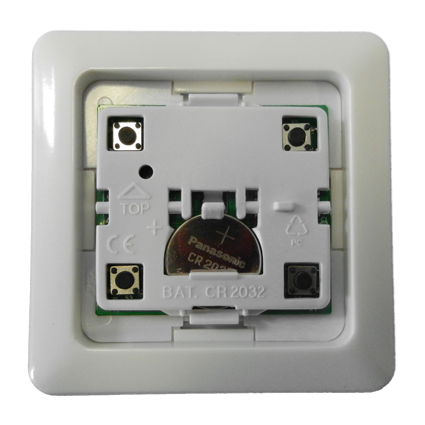
\includegraphics[width=0.4\textwidth]{img/Sensorevaluation/PoppWallController.png}
	\caption{Aufbau des Popp Wall Controllers}
	\label{fig:sensorenPoppController}
\end{figure}

\subsubsection{Buttons}
Die vier Buttons des Schalters können unterschiedlich konfiguriert und genutzt werden. Allgemein ist eine paarweise (Button 1/3 und Button 2/4) und eine separate Verwendung aller Buttons möglich. Außerdem kann Doppelklick aktiviert und deaktiviert werden.

Die Funktionen der Buttons werden über vier "`Command to Control Groups"' definiert und konfiguriert. Diese geben an, welche Kommandos bei Betätigung an assoziierte Geräte gesendet werden. Die Liste der "`Command to Control Groups"' enthalten jeweils neun Einträge.

\begin{itemize}
	\item Disable
	\item Switch On/Off and Dim (send Basic Set and  Switch Multilevel)
	\item Switch On/Off only (send Basic Set)
	\item Switch All
	\item Send Scenes
	\item Send Preconfigured Scenes
	\item Control devices in proximity
	\item Control DoorLock
	\item Central Scene to Gateway
\end{itemize}

\begin{longtabu} to \textwidth{
		>{\hsize=0.9\hsize}X
		>{\hsize=1.2\hsize}X
		>{\hsize=0.9\hsize}X
	}
	% ----------- begin header -----------	
	\hline
	\textbf{Button} &
	\textbf{gepaart} &
	\textbf{separat} \\
	\hline
	\endhead
	% ----------- end header -----------
	% ----------- begin footer -----------
	\multicolumn{3}{r}{{Fortsetzung auf nächster Seite}}  \\
	\endfoot
	\endlastfoot
	% ----------- end footer -----------
	
	Button 1 		& einfacher Klick: Gruppe A & Gruppe A \\
	\cline{1-1} \cline{3-3}
	Button 3		& doppelter Klick: Gruppe C & Gruppe C \\
	\hline
	Button 2		& einfacher Klick: Gruppe B & Gruppe B \\
	\cline{1-1} \cline{3-3}
	Button 4		& doppelter Klick: Gruppe D & Gruppe D \\
	\hline
	
	\caption{Buttons und Assoziationsgruppen des Popp Wall Controllers}
\end{longtabu}

%TODO newpage
%\newpage

Alle Buttons unterstützen verschiedene Klickarten und bieten so Mehrfachfunktionalität. Wenn die Buttons separat verwendet werden, können sie wie folgt geklickt werden:

\begin{description}
	\item [einfaches Klicken] sendet On-Kommando
	\item [doppeltes Klicken] sendet Off-Kommando
	\item [langes Klicken (gedrückt halten)] sendet Dimming-Up-Kommando
	\item [klicken und gedrückt halten]: sendet Dimming-Down-Kommando
\end{description}

\subsubsection{Verwendung als Primärcontroller}
Das Gerät kann als Primärcontroller verwendet werden. In diesem Betriebsmodus wird der Schalter wie ein einfacher Lichtschalter verwendet und bietet ausschließlich die Funktion, eine konfigurierte Lampe an- und auszuschalten. Dazu wird eine direkte, lokale Verbindung zwischen Schalter und Aktor aufgebaut. Es ist kein Gateway erforderlich, welches Befehle vom Schalter entgegennimmt und weiterverarbeitet.

In diesem Betriebsmodus stellt der Schalter alle Funktionen bereit, welche von einem Primärcontroller gefordert werden. Dazu gehört:
\begin{itemize}
	\item Vergabe von Adressen für neu eingebundene Geräte
	\item Aufbauen und Verwalten von Routingtabellen
\end{itemize}

Wird der Schalter als Primärcontroller verwendet, können Aktoren in das lokale, vom Schalter verwaltete Netzwerk eingebunden werden. Bei dieser Inkludierung, geben einzubindende Aktoren ihre Geräteklasse bekannt. Entsprechend dieser Klasse werden anschließend die Buttons des Schalters, bzw. deren Funktion konfiguriert. So können Lampen an- und ausgeschaltet, bzw. gedimmt werden, wenn die Lampen das unterstützen.

Da im gesamten Projekt mit dem Z-Way-Server auf einem Raspberry Pi als Gateway gearbeitet wird, wurde die Verwendung des Schalters als Primärcontroller nicht weitergehend evaluiert.

\subsubsection{Verwendung als Sekundärcontroller}
Als \emph{Sekundärcontroller} kann der Schalter in bestehende Netze eingebunden werden, z.B. in ein von Z-Way verwaltetes Netzwerk. In diesem Modus wird der Schalter über die Oberfläche des Gateways konfiguriert. In diesem Betriebsmodus bietet der Schalter noch mehr Funktionalität. Durch einen Klick auf einen Button können beispielsweise Szenen gestartet werden, z.B. alle Lampen ausschalten. 

Auch wenn der Schalter als Sekundärcontroller verwendet wird, ist es möglich lokale Verbindungen zwischen Schalter und Aktor aufzubauen. \emph{Das ist sehr interessant, da der Schalter so auch Geräte steuern kann, wenn das zentrale Gateway nicht erreichbar oder ausgefallen ist.} Für dieses Verhalten muss über Z-Way-Expert eine Assoziation zwischen Schalter und Aktor hergestellt werden. In dieser Konfiguration werden Kommandos parallel an Gateway und an weitere Assoziationen gesendet (\prettyref{fig:sensorenPoppControllerSek}).

\begin{figure}[h!]
	\centering
	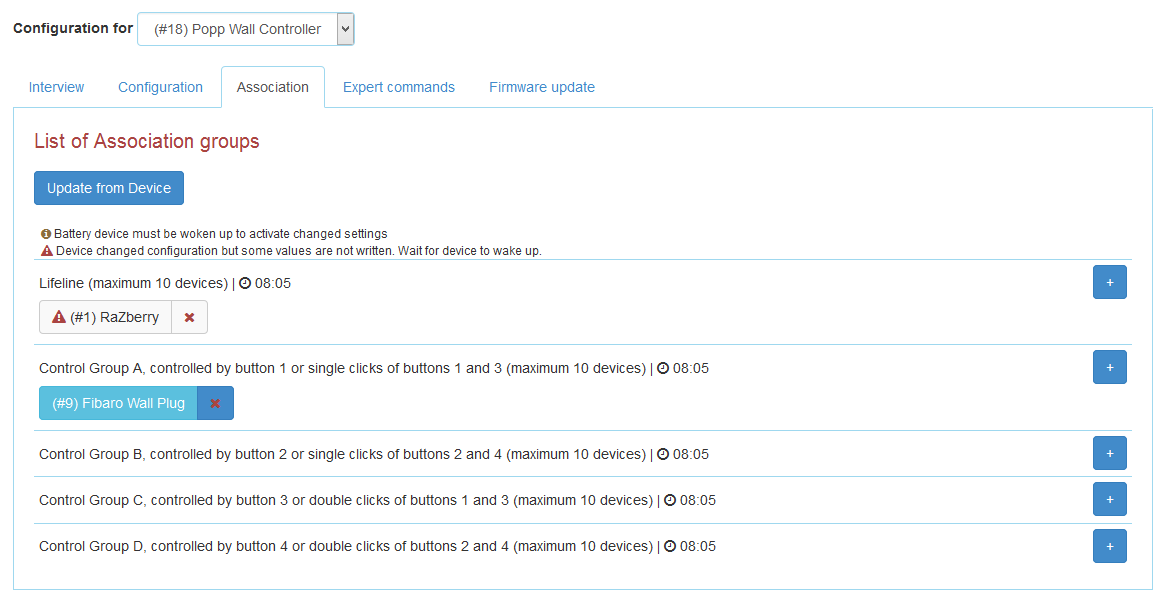
\includegraphics[width=0.9\textwidth]{img/Sensorevaluation/PoppWallControllerSek.png}
	\caption{Z-Way-Oberfläche zur Definition direkter Assoziationen}
	\label{fig:sensorenPoppControllerSek}
\end{figure}

In der Beispielkonfiguration wurde die "`Command to Control Group A"' auf "`Switch On/Off only (send Basic Set)"' gesetzt. Außerdem wurde die Fibaro Schaltsteckdose ("`(\#9) Fibaro Wall Plug"' im Bild oben) als Assoziation für die Gruppe A gesetzt. Somit werden einfache On/Off Kommandos an das Gateway und die Steckdose (\prettyref{subsec:fibaroWallPlug}) gesendet. Auch bei ausgeschaltetem Gateway lässt sich die Steckdose durch den Popp Wall Controller fernsteuern.


\section{Gefahrenquellenabschaltung}
\label{sec:gefahrenquellenabschaltung}

\subsection{Einleitung und Szenariobeschreibung}
Das Szenario "`Gefahrenquellen abstellen"' versucht Ansätze zur Verringerung von Gefahrensituationen im Haushalt, besonders in Bezug auf den Schutz von Kinder, umzusetzen. Dabei werden möglichst viele Informationen durch Sensoren gesammelt, bspw. durch Bewegungssensoren erfasste Daten, mit denen Rückschlüsse über die Präsenz von Personen getroffen werden. Der nächste Schritt ist die Identifizierung von Erwachsenen bzw. Kindern, um Gefahrenquellen abhängig davon abschalten zu können. Um eine mögliche Fehlanalyse der Situation durch das System abzuschwächen soll ein Feedback-Mechanismus die Bewohner über eine auszuführende Aktion informieren und ihnen die Möglichkeit bieten diese abzubrechen. Die Konfiguration der Gefahrenquellen liegt in der Hand des Nutzers.

\subsection{Konzept für die Umsetzung des Szenarios}
Das komplexe Szenario der Gefahrenquellenabschaltung lässt sich nur sinnvoll realisieren, wenn die Funktionalität auf einzelne Module aufgeteilt und entwickelt wird. Zusätzlich wird dadurch eine hohe Wiederverwendbarkeit erreicht.

Nachfolgend werden die erforderlichen Funktionalitäten beschrieben und anschließend, im nächsten Punkt, die entwickelten Module erläutert.

\begin{description}
	\item [Anzahl der Personen in einem Raum] Grundvoraussetzung für das Szenario ist die Information, wie viel Personen sich in einem Raum befinden. Zunächst sollten Gefahrenquellen nur eingeschaltet werden können, falls sich eine Person im Raum befindet und andererseits sollten beim Verlassen des Raums alle Gefahrenquellen ausgeschaltet werden.
	\item [Personenidentifikation] Der Ausbau der erstgenannten Funktionalität besteht in der Identifikation von Kindern und Erwachsenen. Gefahrenquellen dürfen nicht eingeschaltet werden, wenn nur ein Kind im Raum anwesend ist und sollten möglichst zeitnah abgeschaltet werden, sobald ein Erwachsener den Raum verlässt und nur noch ein Kind präsent ist.
	\item [Benachrichtigung anwesender Personen] Es ist nicht sichergestellt, dass alle anwesenden Personen immer zuverlässig erkannt werden. Um die Auswirkungen solcher Fehleinschätzungen des Systems zu reduzieren, sollen eventuell anwesende Personen benachrichtigt werden. Dies kann z.B. durch optische Signale geschehen. Dafür ist eine gewisse Zeitspanne festgelegt, in der die anwesenden Personen die Möglichkeit haben, die anstehende Aktion zu unterbrechen.
	\item [Gefahrenquellen ausschalten] Um den Schutz bestmöglich zu gewährleisten muss der Bewohner, die im Haus befindlichen Gefahrenquellen auswählen können, welche bei Erkennen, dass sich nur ein Kind im Raum befindet, abgeschaltet werden.
\end{description}


\subsection{Umsetzung und Programmierung, entwickelte Module}
Aus den oben beschriebenen Funktionalitäten wurden die im folgenden beschriebenen Module entwickelt. Diese arbeiten eng zusammen und bieten teils spezielle Funktionen, welche für sich genommen wenig nützlich erscheinen.
\begin{description}

\item [PersonCounterModule] Das \emph{PersonCounterModule} bietet eine Schnittstelle um die Anzahl der Personen innerhalb eines Raumes zum derzeitigen Zeitpunkt zu speichern und bereitzustellen. Diese Information kann von Modulen verändert werden, die festellen können ob Personen den Raum betreten oder verlassen haben. Jedes Modul, welches Informationen zur derzeitigen Personenanzahl benötigt, kann auf die Informationen des \emph{PersonCounter} im jeweiligen Raum zurückgreifen.

\item [RoomAccessModule] Um ein Betreten und Verlassen eines Raumes an einem Türdurchgang zu überprüfen wird das \emph{RoomAccessModule} benutzt. Dazu werden Bewegungssensoren auf jeder Seite der Tür benötigt. Die \emph{PersonCounter} der angrenzenden Räume werden jeweils den Sensoren zugeordnet. Dadurch kann eine Bewegungsrichtung und damit ein Betreten und Verlassen eines Raumes festgestellt werden.

\item [PersonIdentifikatorModule] Zusätzlich kann an einem Türdurchgang ein weiterer Bewegungssensor angebracht werden um zu definieren ob die Person die einen Raum betritt bzw. verlässt, ein Erwachsener oder ein Kind ist. Dies wird während des Betreten und Verlassen des Raums überprüft und hält damit zusätzliche Informationen zu den anwesenden Personen. Des Weiteren findet eine weitere Überprüfung über den weiteren Verlauf des CO$_2$ Gehalts in der Luft statt, um die Höhenmessung an der Tür zu bestätigen.

\item [InHomeFeedbackModule] Das \emph{InHomeFeedbackModule} kann benutzt werden um den Nutzern im Raum eine Rückmeldung zu anstehenden Aktionen im Raum zu geben. Dieser kann dann notfalls darauf reagieren und die anstehenden Aktionen abbrechen. Dieser wird über einen ZAutomation-Aufruf auf dem entsprechenden \emph{InHomeFeedbackModule} gestartet. Genau wie \emph{PersonCounter} existieren \emph{InHomeFeedbackModule} je Raum.

\item [TurnOffTimerModule] Wird erkannt das kein Erwachsener mehr im Raum ist startet ein \emph{Timer} der ein Signal an das \emph{InHomeFeedbackModule} weitergibt. Während Ablauf des Timers ist das \emph{InHomeFeedbackModule} aktiv. Wird eine Aktion vom Nutzer während des Zeitraums vorgenommen, wird dies berücksichtigt.

\item [TurnOffHazardModule] Nach Ablauf des \emph{Timers} wird ein Aufruf an das \emph{TurnOffHazardModule} gesendet. Dieser schaltet nun alle definierten Gefahrenquellen ab. Sollte erneut ein Erwachsener erkannt werden können, sofern gewünscht, können die Gefahrenquellen erneut aktiviert werden.
\end{description}


\subsection{Beschreibung des Versuchsaufbau und verwendeter Sensoren}
In einem Versuchsaufbau wurde das oben beschriebene Szenario mit den genannten Modulen realisiert. Die Module wurden wie beschrieben konfiguriert und erstellt. Da schon bei der Entwicklung der Module ausführlich getestet wurde, traten an dieser Stelle keine Probleme auf.
Für den Versuchsaufbau wurden folgende Geräte verwendet:

\begin{description}
\item [Philio und Fibaro Bewegungssensor] Für die Personenerkennung und Zählung an der Tür wurden Bewegungssensoren verwendet. Am besten für einen Türdurchgang sind die Fibaro Bewegungssensoren zu verwenden, da diese auf eine minimale Reaktionszeit von einer Sekunde konfigurierbar sind, d.h. jede Sekunde kann eine Bewegung erkannt werden. Andere vorhandene Bewegungssensoren sind träger und lassen nur eine weitaus höhere Reaktionszeit von 10 bis 18 Sekunden zu, was vorallem bei einem Szenario mit mehreren Personen von Nachteil ist.

\item [Sensoair CO$_2$ Sensor und Aeotec Bewegungssensor] Zur Personenidentifikation wird zum einen der Aeotec Bewegungssensor verwendet, um einen Erwachsenen zu erkennen. Zum anderen wird der CO$_2$ Sensor benutzt um die Erkennung des Bewegungssensors zu überprüfen.

\item [Popp Wall Controller] Der Schalter wird verwendet, um das \emph{InHomeFeedbackModule} zu steuern. Doppeltes Klicken des Button 2 bewirkt, dass ein laufendes Feedback abgebrochen wird und somit die Anwesenheit von Personen signalisiert wird.

\item [Fibaro Wall Plug] Der schaltbare Zwischenstecker mit einer angeschlossenen Schreibtischlampe wird vom \emph{InHomeFeedbackModule} genutzt. Bei Aktivierung des Feedback-Modus schaltet die Steckdose sekündlich an und aus.

\item [Gefahrenquelle] Hier simuliert dargestellt als ein Dummy Modul, was ein Bügeleisen darstellen soll. Dieses Gerät wird letztendlich vom \emph{TurnOffHazardModule} nach Ablauf des Timers deaktiviert.
\end{description}

Folgender theoretischer Ablauf findet in diesem Szenario statt:
\begin{longtabu} to \textwidth{
		>{\hsize=0.8\hsize}X
		>{\hsize=1.2\hsize}X
	}
	\hline
	\textbf{Aktionen des Benutzers}									& \textbf{Reaktion des Systems} \\
	\hline
	\endhead
	Erwachsener betritt den Raum	& Personenzähler erhöht Personenzahl im Raum um eins, Personidentifikator erkennt Person als Erwachsener anhand der Höhenmessung, start der CO$_2$ Messung zur Bestätigung des Ergebnisses der Höhenmessung \\
	\hline
	Kind betritt den Raum	& Personenzähler erhöht Personenzahl im Raum um eins, Personidentifkator erkennt Person als Kind anhand der Höhenmessung, start der CO$_2$ Messung zur Bestätigung des Ergebnisses der Höhenmessung \\
	\hline
	Erwachsener fängt an zu Bügeln	& - \\
	\hline
	Erwachsener beendet bügeln und lässt Bügeleisen an	& - \\
	\hline
	Erwachsener verlässt den Raum	& Personenzähler vermindert Personenzahl im Raum um eins, Personidentifikator erkennt Person als Erwachsener anhand der Höhenmessung, start der CO$_2$ Messung zur Bestätigung des Ergebnisses der Höhenmessung, Feedbackmodul und Timermodul wird aktiviert \\
	\hline
	-	& Nach dem Ablauf des Timers wird das Feedbackmodul deaktiviert und das Bügeleisen abgeschalten. \\
	\hline
	Erwachsener betritt den Raum	& Personenzähler erhöht Personenzahl im Raum um eins, Personidentifikator erkennt Person als Erwachsener anhand der Höhenmessung, start der CO$_2$ Messung zur Bestätigung des Ergebnisses der Höhenmessung \\
	\hline
	Erwachsener betätigt Schalter an schaltbarer Steckdose des Bügeleisens 	& Bügeleisen ist wieder angeschalten \\
	\hline
	\caption{TurnOffTimerModule: Schnittstelle Event Bus}
\end{longtabu}


\subsection{Zusammenfassung}
Das Szenario ist größtenteils nach dem oben ablaufenden Schema durchführbar. Die Module und Sensoren für einen solchen Ablauf sind vorhanden. Einzelne Modul- und Sensortests waren erfolgreich. In der Praxis jedoch sind während des Integrationstests sowohl Module als auch Sensoren im Z-Way-Server ausgefallen und waren erst nach einem Neustart des Servers verfügbar. Die anfänglichen Schwierigkeiten konnten relativ zügig behoben werden und verschieden Testfälle führten zu einem positiven Ergebnis. Die Kombination aus CO$_2$- und Größenmessungen lieferten dabei eine akzeptable Abschätzung über die im Raum befindlichen Personen.


\section{Alarmanlage}
\subsection{Einleitung und Szenariobeschreibung}
Das Szenario "`Haus/Wohnung bei verschließen der Haus-/Wohnungstür in Standby versetzten"' wurde entwickelt, um Nutzern bei Verlassen des Hauses möglichst hohen Komfort zu bieten. Dazu sollen verschiedene Aktionen gestartet werden, sobald der letzte Bewohner das Haus verlässt. Es ist von herausragender Bedeutung zu wissen, ob noch Personen anwesend sind, oder wirklich niemand mehr zu Hause ist. Wenn das der Fall ist, kann das Haus in den Standby-Modus versetzt werden. Dazu können verschiedene Geräte abgeschaltet und eine Alarmanlage aktiviert werden.

\subsection{Konzept für die Umsetzung des Szenarios}
Das oben beschriebene Szenario bringt einige Komplexität mit sich, welche nur schwer auf ein einzelnes Modul abbildbar ist. Aus diesem Grund wurde die zu erbringende Funktionalität analysiert und in überschaubare Funktionseinheiten gegliedert, diese werden wiederum durch einzelne Module repräsentiert. Außerdem bietet die Implementation verschiedener Module zur Bereitstellung einzelner Funktionseinheiten den Vorteil hoher Wiederverwendbarkeit.

Im Folgenden werden erforderte Funktionalitäten beschrieben und darauf folgend die aus den Anforderungen entwickelten Module.

\begin{description}
	\item [Verlassen der Wohnung] Ausgangspunkt des Szenarios ist das Verlassen der Wohnung. Falls die Wohnungstür mit einem intelligenten, vernetzten Türschloss ausgestattet ist, signalisiert dieses beim Verschließen, dass der Standby-Modus aktiviert werden kann. Zu diesem Zeitpunkt wird dieser Modus jedoch nicht instantan aktiviert, dazu sind noch weitere Überprüfungen erforderlich. Ist in der Wohnung kein entsprechendes Schloss vorhanden, kann dieses auch durch einen Schalter in der Nähe der Wohnungstür ersetzt werden.
	\item [Ankommen in der Wohnung] Beim Aufschließen der Wohnungstür wird der Standby-Modus automatisch deaktiviert. Das heißt evtl. aktivierte Alarmanlagen werden deaktiviert oder entsprechend konfigurierte Geräte an- bzw. abgeschaltet.
	\item [Überprüfen der Personenanzahl] Bevor der Standby-Modus der Wohnung aktiviert werden kann, ist es erforderlich zu überprüfen, ob Personen anwesend sind. Sollten sich Personen in der Wohnung aufhalten, darf der Standby-Modus nicht aktiviert werden, da anwesende Personen sonst in ihrer Aktivität gestört würden.
	\item [Benachrichtigen Anwesender] Es ist nicht sichergestellt, dass alle anwesenden Personen immer zuverlässig erkannt werden. Um die Auswirkungen solcher Fehleinschätzungen des Systems zu reduzieren, sollen eventuell anwesende Personen benachrichtigt werden. Dies kann z.B. durch optische Signale geschehen. Dafür ist eine gewisse Zeitspanne festgelegt, in dieser haben anwesende Personen die Möglichkeit, die anstehende Aktion zu unterbrechen. Folglich kann der Standby-Modus in dieser Zeitspanne nicht aktiviert werden. Das stellt allerdings kein Problem dar, da es unerheblich ist, wie schnell genau nach Verlassen der Wohnung der Standby-Modus aktiviert wird.
	\item [Geräte in Standby schalten] Wenn davon ausgegangen werden kann, dass sich keine Personen mehr in der Wohnung aufhalten, kann der Standby-Modus aktiviert werden. Infolgedessen werden konfigurierte Geräte, wie zum Beispiel Steckdosen oder Lampen, ausgeschaltet. Außerdem können Orientierungsleuchten oder Geräte zur Überwachung angeschaltet werden.
	\item[	Alarmanlage aktivieren] Die Aktivierung der Alarmanlage ist nur sinnvoll, wenn sich keine Person in der Wohnung befindet. Deshalb ist es sinnvoll, die Aktivierung der Alarmanlage an die Standby-Schaltung zu koppeln. Nach Aktivierung des Standby-Modus kann die Alarmanlage aktiviert werden. Somit wird die Gefahr von Fehlalarmen reduziert.
\end{description}

\subsection{Umsetzung und Programmierung, entwickelte Module}
Aus den oben beschriebenen Funktionalitäten wurden die im folgenden beschriebenen Module entwickelt. Diese arbeiten eng zusammen und bieten teils spezielle Funktionen, welche für sich genommen wenig nützlich erscheinen.
\begin{description}
	\item [LockDoorModule] Das \emph{LockDoorModule} übernimmt die Koordination der oben beschriebenen Funktionen. Da sich diese Aufgaben immer auf die Wohnung als Ganzes beziehen, wurde das Modul als Singleton konzipiert und kann deshalb nur einmalig angelegt werden. Zur Überprüfung der Personenanzahl wird die ZAutomation-Schnittstelle aller verfügbarer \emph{PersonCounter} verwendet. Wenn endgültig keine Personen erkannt wurden, sendet das \emph{LockDoorModule} ein Event auf dem Event Bus. Abbonenten werden darüber informiert, dass sich keine Personen in der Wohnung befinden und können entsprechende Aktionen ausführen. 
	
	\item [PersonCounterModule] Das \emph{PersonCounterModule} stellt eine Schnittstelle zur Zählung der Personen je Raum bereit. Dazu können verschiedene Sensoren genutzt werden, detaillierter wird dies unter "`Gefahrenquellenabschaltung"' (\prettyref{sec:gefahrenquellenabschaltung}) beschrieben.
	
	\item [InHomeFeedbackModule] Falls durch die \emph{PersonCounter} keine Personen erkannt wurden, startet das \emph{LockDoorModule} den Feedback-Modus. Auch dieser wird über einen ZAutomation-Aufruf auf dem entsprechenden \emph{InHomeFeedbackModule} gestartet. Genau wie \emph{PersonCounter} existieren \emph{InHomeFeedbackModule} je Raum.
	
	\item [StandbyModule] Nach Überprüfung der oben beschriebenen Sachverhalte beim Abschließen der Wohnung tritt das \emph{StandbyModule} in Aktion. Auch dieses Modul existiert nur einmalig für die gesamte Wohnung. Die Konfiguration erlaubt das Festlegen von Regeln sowohl für das Betreten als auch das Verlassen des Standby-Modus.
	
	\item [AlarmModule] Wie auch das \emph{StandbyModule} funktioniert der Alarm im Zusammenhang mit dem \emph{LockDoorModule}. Erst nachdem ein entsprechendes Event empfangen wurde, aktiviert das \emph{AlarmModule} die Alarmanlage. Dazu werden verschiedene Sensoren auf Statusänderungen überwacht und bei der Erkennung von Aktivitäten genutzt.
\end{description}

\subsection{Beschreibung des Versuchsaufbau und verwendeter Sensoren}
In einem Versuchsaufbau wurde das oben beschriebene Szenario mit den genannten Modulen realisiert. Die Module wurden wie beschrieben konfiguriert und erstellt. Da schon bei der Entwicklung der Module ausführlich getestet wurde, traten an dieser Stelle keine Probleme auf.
Für den Versuchsaufbau wurden folgende Geräte verwendet:

\begin{description}
	\item [Popp Wall Controller] Dieser Wandschalter wird genutzt, um ein Türschloss zu simulieren. Durch einfaches Klicken auf den Button 1 kann das Verschließen, durch drücken auf Botton 3 das Aufschließen der Tür simuliert werden. Außerdem wird der Schalter verwendet, um das \emph{InHomeFeedbackModule} zu steuern. Doppeltes Klicken des Button 2 bewirkt, dass ein laufendes Feedback abgebrochen wird und somit die Anwesenheit von Personen signalisiert wird.
	
	\item [Philio 4-in-1 Multisensor] Der Tür- und Fensterkontakt dieses Sensors wird als Auslöser für die Alarmanlage genutzt. Wurde die Wohnung verschlossen und das \emph{AlarmModule} aktiviert, werden Zustandsänderungen des Kontakts als Einbruch interpretiert. Daraufhin wird der Alarm aktiviert. Da keine entsprechende Sirene zur Verfügung steht, setzt das \emph{AlarmModule} einen HTTP-Request ab, lässt eine Website blinken und spielt dort einen Alarmton ab.
	
	\item [Fibaro Wall Plug] Der schaltbare Zwischenstecker mit einer angeschlossenen Schreibtischlampe wird vom \emph{InHomeFeedbackModule} genutzt. Bei Aktivierung Feedback-Modus schaltet die Steckdose sekündlich an und aus.
	
	\item [Weitere Bewegungsmelder] Für die Personenerkennung und Zählung an der Tür wurden weitere Sensoren (insbesondere Bewegungsmelder) verwendet. Da diese nicht in direktem Zusammenhang mit dem \emph{AlarmModule} stehen, wird deren Verwendung hier nicht näher beschrieben, statt dessen sei auf den Abschnitt "`Gefahrenquellenabschaltung"' (\prettyref{sec:gefahrenquellenabschaltung}) verwiesen.
\end{description}
\subsection{Zusammenfassung}
Das Szenario konnte wie ursprünglich beschrieben umgesetzt werden, wiewohl Erweiterungen denkbar sind. Beispielsweise kann das \emph{AlarmModule} für die Konfiguration weiterer Geräte erweitert werden, welche in einem Alarmfall aktiviert werden.

Die Einbindung eines vernetzten Türschlosses ist zwar angedacht, konnte jedoch nicht getestet werden. Geringfügige Anpassungen in den einzelnen Modulen sollten dies jedoch einfach ermöglichen.


%%%%%%%%%%%%%%%%%%%%%%%%%%%%%%%%%%%%%%%%%%%%%%%%%%%%%%%%%%%%%%%%%%%%%%%%%%%%%%%%
\newpage
\section{Feedback-Mechanismen}
\label{sec:feedbackMechanismen}
\emph{(von Zarina Muratbekovna Omurova)}

\noindent
Bisher wurde davon ausgegangen, dass für ein leistungsfähiges intelligentes Haus Feedback-Möglichkeiten vorhanden sein sollen. Orientiert man sich an den Fähigkeiten des Menschen, sind dies das menschliche Sehen, Hören, Fühlen , Bewegen, Riechen und Schmecken. Insbesondere das Sehen, Hören und Bewegen sind für Feedbacks von Bedeutung. Als Möglichkeit für eine Rückmeldung stehen Displays, akustische Systeme und Gesten zur Verfügung. Um nun geeignete Reaktionen zu erwirken, bedarf es einer in Grenzen leistungsfähigen Systemintelligenz. Hierdurch wird die Repräsentation durch mögliche Interaktionen mit dem Smart Home möglich und hilft, den Eindruck von \glqq Intelligenz\grqq{} zu vermitteln. Auch dies ist eine wichtige Eigenschaft für die flexible Anpassungsfähigkeit an die vom Nutzer vorgegebenen Aufgabenstellungen. Die Anforderungen richten sich gleichermaßen, sowohl an sensorische Fähigkeiten als auch an die Fähigkeit, Daten von Sensoren in Erkenntnisse zu transformieren und daraus Strategien und Konzepte zu entwickeln. Methoden zur Wahrnehmung der Umwelt sowie zur Kommunikation mit dieser, stehen seit Jahren im Fokus der Forschung.\\
Im folgenden werden einige Forschungsarbeiten vorgestellt die im Laufe der Ausarbeitung entdeckt wurden. Unter anderem werden Möglichkeiten beschrieben die später in dem Projekt als Feedback eingesetzt werden können. Es werden auch schon vorhandene Lösungen auf dem Markt vorgestellt, die übernommen werden können. Es soll auch der Kostenfaktor berücksichtigt werden, da es nicht bekannt ist, ob die teuren Lösungen in dem Projekt eingesetzt werden können.\\
Weiter unten werden am Markt vorhandene Systeme und Lösungen kurz aufgelistet.\\

\subsection{Steuermechanismen auf Basis von Akustik}
\acrfull{tts} wandelt Fließtext in eine akustische Sprachausgaben um. Diese Technologie wird von den meisten Sprachmechanismen benutzt.

\begin{figure}[h!]
	\centering
	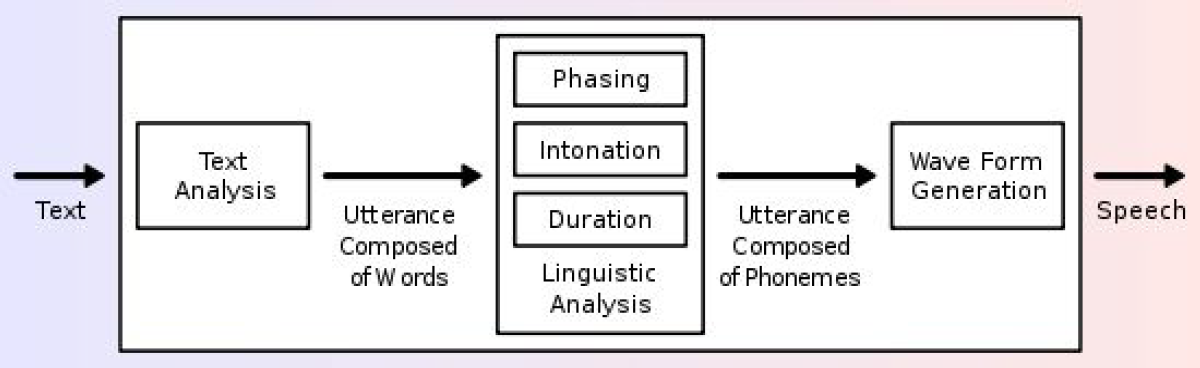
\includegraphics[width=0.9\textwidth]{img/Feedback-Mechanismen/TTS.png}
	\caption{\gls{tts}}
	\label{fig:feedbackTTS}
\end{figure}

Der Einsatz von sprach-gesteuerten Systemen hat bereits auf verschiedensten Gebieten, mehr oder weniger erfolgreich Einzug gehalten.

\subsubsection{IVEE}
Die nachfolgenden Ausführungen beziehen sich auf die Onlinequelle \glqq Deine Sprachsteuerung für dein SmartHome\grqq\footnote{\url{http://www.siio.de/connected-home/ivee-deine-sprachsteuerung-fuer-dein-smarthome/}}.

\begin{itemize}
\item Kosten: 200\$
\end{itemize}

\noindent
Bei ivee handelt es sich um eine cloudbasierte Sprachsteuerung für das Smart Home, bei der vom Marktstart an bereits diverse Hersteller angebunden sind. Hervorzuheben sind hier Belkin WeMo, Philips Hue, Logitech Harmony \& Google Nest sowie Z-Wave. Zu den genannten Anbietern werden kontinuierlich Neue dazu kommen. Nützlich könnten hier zum Beispiel eine Anbindung durch \gls{iftttg} oder an Google sein. Mit \gls{iftttg} könnten mit einem Schlag eine Vielzahl weiterer Dienste angebunden werden und mit der Anbindung an Google könnte man sich neue Mails oder Kalendereinträge vorlesen lassen. Die Installation und Steuerung von ivee ist auch für wenig technisch versierte Personen einfach umzusetzen. Die Sprachsteuerung ivee muss dazu nur an den Strom angeschlossen – und ins heimische WLAN integriert werden. Mit der dazugehörigen Smartphone App kann ivee beigebracht werden, welche Geräte im Haushalt verfügbar sind. Auch die Steuerung ist denkbar einfach:

\begin{enumerate}
\item Sag einfach \glqq Okay ivee\grqq{} zum Aufwecken. Der eingebaute, farbige LED-Ring wird blau und das System ist bereit für den Sprachbefehl.
\item Dann einfach das Kommando sagen oder die Frage stellen. Zum Beispiel: \glqq Schalt den Fernseher ein\grqq .
\item ivee schaltet den Fernseher an.\\
\end{enumerate}

Mit der iPhone-App können auch unterschiedliche Szenen angelegt werden, die zum Beispiel bei einem bestimmten Kommando die HUE-Leuchten dimmen, den Fernseher anschalten und die Raumtemperatur erhöhen. Alles möglich.

\begin{figure}[h!]
	\centering
	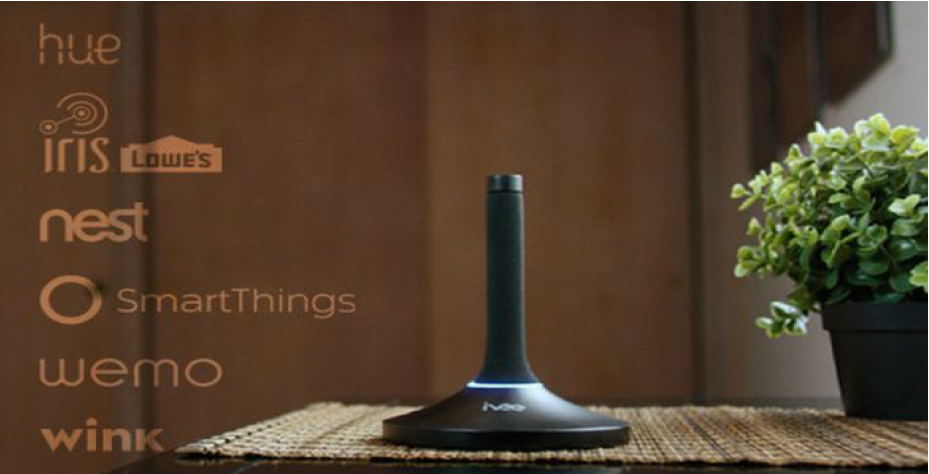
\includegraphics[width=0.9\textwidth]{img/Feedback-Mechanismen/IVEE.png}
	\caption{IVEE}
	\label{fig:feedbackIVEE}
\end{figure}

Art des Feedbacks: Es kann mit ivee Dialog ausgeführt werden, als Feedback erhält eine Person von ivee eine sprachliche Bestätigung zurück, die mittels eingebaute Mikrofone übermittelt wird, das die Aktion ausgeführt wurde.

\subsubsection{CastleOS Voice}
Die nachfolgenden Ausführungen beziehen sich auf die Onlinequelle \glqq CastleOS Voice-Controlled Home Automation Software for INSTEON, Z-Wave, WeMo, and More\grqq\footnote{\url{http://www.smarthome.com/castleos-voice-controlled-home-automation-software-for-insteon-z-wave-wemo-and-more.html}}.

\begin{itemize}
\item Kosten: 200\$
\end{itemize}

\noindent
CastleOS Voice-Controlled Home Automation Betriebssystem für INSTEON, X10, Z-Wave, UPB, LightwaveRF, WeMo, Nest, Sonos, Plex, XBMC, MediaBrowser3, DirecTV. Es ist kompatibel mit folgenden Smart Home Geräten wie Aeon Labs, Yale, Phillips, Honeywell, GE, Leviton, Sonos. CastleOS verwendet eine einzigartige Dual-Gerätesteuerung, die einfache Sprachbefehle durch eine Kinect oder CastleOS Web- und Mobile-Anwendung auf jedem iOS und Android Gerät akzeptiert. Befehle werden von der Kinect oder Web- und Mobile-Anwendung auf einen Windows PC, der mit einer unbegrenzten Anzahl von verbundenen Heimautomatisierungsgeräte, wie INSTEON, Z-Wave, UPB, X10 oder WeMo weitergeleitet. CastleOS kann nicht nur auf Sprachbefehle reagieren, sondern auch mit dem Ton Bestätigungen und Antworten auf Fragen und Befehle zu ausgeben. Kinect ermöglicht eine vollständige Kontrolle über ihr Zuhause mit einem präzisen und anspruchsvollen Spracherkennungssystem. Ihr Haus wird 24/7 ohne Störungen durch laute Musik, Filme, TV und andere Geräusche überwacht. Es gibt keine Begrenzung für die Anzahl der Kinect-Geräte die angeschlossen werden können aber zusätzliche Kinects erhöhen den Standard Übertragungsbereich um bis zu 10 Meter. Es kann auch mittels Mobil- bzw. Webapp gesteuert werden, falls keine Kinect vorhanden ist.

\begin{table}[H]
	\begin{tabularx}{\textwidth}{
			>{\hsize=0.5\hsize}X 
			>{\hsize=1.5\hsize}X
			% sum=2.0\hsize for 2 columns
		}
		\hline
		Betriebssystem	
		& Windows 7 oder neuer \\
		\hline 
		Z-Wave
		& Aeon Labs Z-Stick \\
		\hline
	\end{tabularx}
	\caption{Systemanforderungen: CastleOS}
\end{table}

\begin{table}[H]
	\begin{tabularx}{\textwidth}{
			>{\hsize=0.5\hsize}X 
			>{\hsize=1.5\hsize}X
			% sum=2.0\hsize for 2 columns
		}
		\hline
		Kompatibilität	
		& INSTEON, Z-Wave, UPB, WeMo \\
		\hline 
		Sprachsteuerung
		& mit Kinect und Kinect Voice Interface, Reichweite: 10,66 m, natürliche Sprachbefehle \\
		\hline 
		Gerätegruppierung
		& Szene, Gruppe \\
		\hline
	\end{tabularx}
	\caption{Features: CastleOS}
\end{table}

Die Änderungen, die mit Version CastleOS 2.0 erscheinen sollen, werden die Erstellung von virtuellen Geräten und Protokollen ermöglichen. Auf diese Weise können beliebige HTTP-Aufrufe ausgeführt werden. Der endgültige Termin ist nicht festgelegt, laut  Q\&A auf der offiziellen Webseite wird es noch dauern bis es in die Produktion geht.

\glqq The REST API was added a few months ago to support Android App development. To discover the services, you can use any web service explorer and point it to CastleOS on your machine: \url{http://localhost/CastleOS/service?wsdl}. You can also put that address in your web browser to see the raw XML if you'd like. The Custom Scripting as an Action is in testing now, and will be in the next release.\grqq

\subsubsection{Amazon Echo}
Die nachfolgenden Ausführungen beziehen sich auf die Onlinequelle \glqq Amazon hört und spricht ins Wohnzimmer\grqq\footnote{\url{http://www.golem.de/news/amazon-echo-amazon-hoert-und-spricht-ins-wohnzimmer-1411-110371.html}}

\begin{itemize}
\item Kosten: 179,99\$
\end{itemize}

\noindent
Der Echo kann jetzt auch Belkin WeMo und Philips Hue Produkte steuern. Amazon Echo sieht aus wie ein kleiner Bluetooth-Lautsprecher, der aber viel mehr kann als nur Musik abzuspielen. Das Gerät ist per WLAN mit dem Internet verbunden und besitzt sieben Mikrofone, mit denen es jedes Gespräch im Raum registrieren kann. Eine Fernbedienung mit eingebauten Mikrofonen, welche benutzt werden kann, wenn der Hub außer Reichweite ist, steht zur Verfügung.

\begin{table}[H]
	\begin{tabularx}{\textwidth}{
			>{\hsize=0.5\hsize}X 
			>{\hsize=1.5\hsize}X
			% sum=2.0\hsize for 2 columns
		}
		\hline
		WiFi	
		& zur Einbindung in das Heimnetz \\
		\hline 
	 	Bluetooth
		& Audiostreaming für Amazon Echo Mobilgeräte, Fernbedienung \\
		\hline 
	 	Systemanforderungen
		& Zugriff über Mobile-App oder Weboberfläche \\
		\hline
	\end{tabularx}
	\caption{Spezifikation: Amazon Echo}
\end{table}

\begin{figure}[h!]
	\centering
	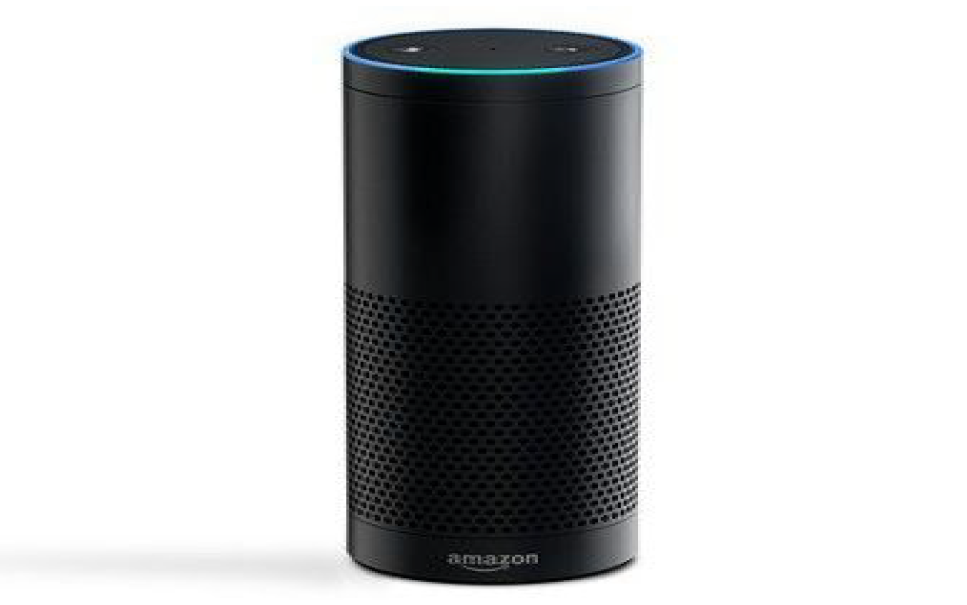
\includegraphics[width=0.9\textwidth]{img/Feedback-Mechanismen/AmazonEcho.png}
	\caption{Amazon Echo}
	\label{fig:feedbackAmazonEcho}
\end{figure}

Eine Anleitung zur Anbindung an Z-Wave ist unter \url{http://www.myzwave.net/index.php/adding-voice-control-to-vera-z-wave-systems-using-amazon-echo/2/} zu finden.

Die nachfolgenden Ausführung beziehen sich auf die Onlinequelle \glqq Amazon\grqq\footnote{\url{http://www.amazon.com/dp/B00X4WHP5E}} und \glqq Smart Home - Home Automation Superstore\grqq \footnote{\url{http://www.smarthome.com/amazon-echo-alexa.html}}.

Amazon Echo kommuniziert visuell mit dem Benutzer über sein Status mit Hilfe einer farbigen Beleuchtung ganz oben und unten:

\begin{figure}[h!]
	\centering
	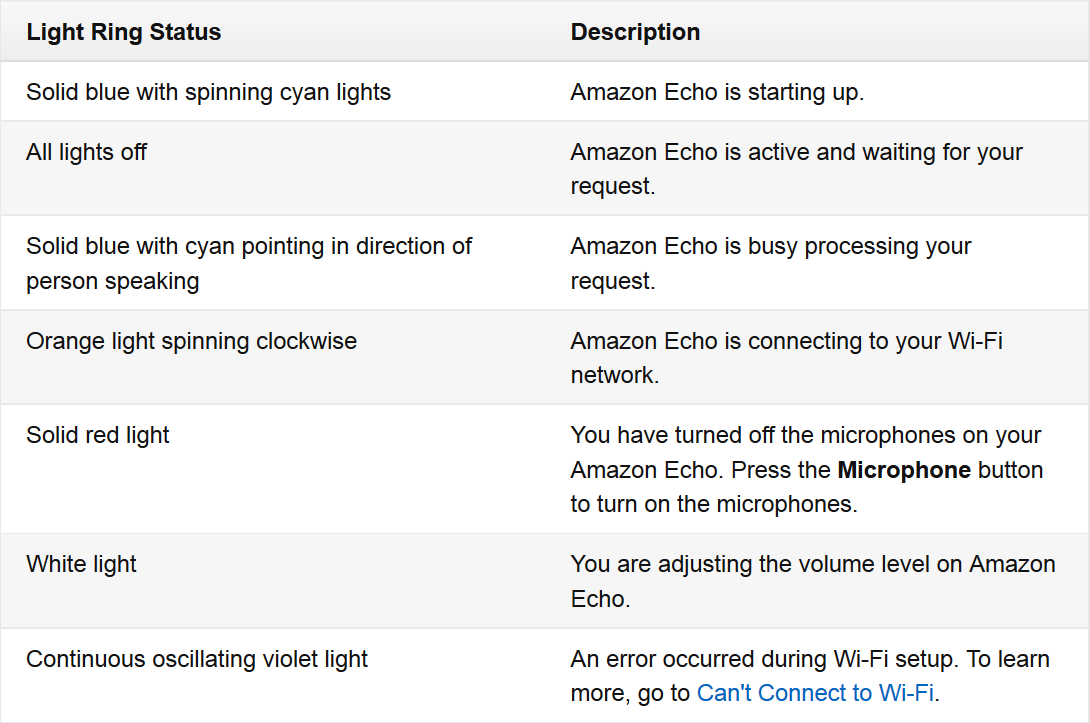
\includegraphics[width=0.9\textwidth]{img/Feedback-Mechanismen/AmazonEchoLight.png}
	\caption{Amazon Echo - Beleuchtung}
	\label{fig:feedbackAmazonEchoLights}
\end{figure}

Wenn ein Befehl ausgelöst wurde, wird Amazon Echo mit \glqq OK\grqq{} zurück antworten, wenn z.B gesagt wurde \glqq Licht an\grqq , wird \glqq OK\grqq{} ausgegeben.

How to control Z-Wave devices with amazon echo via SmartThings hub (\url{http://misterhouse.blogspot.de/2015/10/amazon-echo-smartthings-howto.html})

Die Z-Wave Geräte können von Amazon Echo mithilfe von SmartThings Hub gesteuert werden. In
Amazon App Einstellungen wird Amazon zu Smartthings verlinkt, und danach können alle Geräte
identifiziert werden. Nachdem die Geräteidentifizierung abgeschlossen ist, kann der Nutzer seine Geräte schon per Amazon Echo steuern.

Mit Amazon-Echo-ha-bridge wird ein Hue Hub emuliert, und es können vom Benutzer virtuell erstellte Geräte von diesem Hub identifiziert werden. Diese Geräte können konfiguriert werden um HTTP Rest Befehle zu den anderen Geräten im Haus senden und diese steuern zu können.

HowTo Amazon-Echo-Bridge (\url{https://github.com/armzilla/amazon-echo-ha-bridge})

\noindent
\glqq HowTo: Using Echo to control SmartThings:
Amazon-echo-ha-bridge which is a Java application that emulates a Hue/WeMo hub. The user can
create virtual \glqq lights\grqq{} that Echo will discover using it's native Hue/WeMo support. You can configure the \glqq lights\grqq{} to send HTTP REST commands to other systems in your house. You can say \glqq turn on the <xxx>\grqq , \glqq turn off the <yyy>\grqq , or \glqq set the <zzz> to 50\%\grqq{} (or whatever value). These are utilizing the on/off/dim verbs that Echo understands for light controls, so it works best for activities that would make sense in this sort of sentence. \glqq Alexa, set the thermostat to 78 percent\grqq{} might be ok for setting the temperature.\grqq

\subsubsection{Homey}
Die nachfolgenden Ausführungen beziehen sich auf die Onlinequelle \glqq Homey, preheat the oven! This orb lets you control your house with your voice\grqq\footnote{\url{http://www.digitaltrends.com/home/homey-adds-jarvis-style-voice-control-practically-everything-house/}}

\begin{itemize}
\item Kosten: 299,00€
\end{itemize}

\noindent
Homey unterstützt auch Dinge wie NFC, nRF24L01 + und Infrarot, sowie Z-Wave, ZigBee,
Bluetooth und WiFi. Es wird verwendet, um TV, nicht vernetzte Soundsysteme zu steuern und sogar
Computer. Der Vorteil ist das Homey eine natürliche Sprache versteht. Es sollen keine Befehle in einer bestimmten Reihenfolge ausgesprochen werden, um mit dem Homey zu interagieren. Homey ist mit einem \emph{natural language} Prozessor ausgestattet und versteht die Kurzbefehlen die zur Hausautomatisierung ausgerichtet sind. Es können folgende Befehle wie z.B. \glqq Heizung an\grqq , \glqq Tür zu\grqq{} oder \glqq Licht an\grqq{} ausgesprochen werden und es wird vom System verstanden. Homey ist mehrsprachig, u.a Deutsch.

\begin{figure}[h!]
	\centering
	\includegraphics[width=0.9\textwidth]{img/Feedback-Mechanismen/Homey.png}
	\caption{Homey}
	\label{fig:feedbackHomey}
\end{figure}

Mit REST API, kann der Benutzer mit Homey interagieren und von außen HTTP Anfragen senden
um die Geräte zu steuern. Die Verwendung ist unter \url{https://developers.athom.com/api/#} erklärt.

\subsubsection{EnBlink}
Die nachfolgenden Ausführungen beziehen sich auf die Onlinequellen \glqq Enblink dongle now lets you control smart home devices with voice commands\grqq\footnote{\url{http://www.digitaltrends.com/home/enblink-dongle-now-lets-control-smart-home-devices-voice-commands/}} und \glqq Smart Home - Home Automation Superstore\grqq\footnote{\url{http://www.smarthome.com/enblink-ss201-us-w-z-wave-usb-plug-in-controller.html}}.

\begin{itemize}
\item Kosten: 89,99\$
\end{itemize}

\noindent
Es handelt sich hierbei um einen kleine USB-Stick, der in jedes Google-TV-Gerät gesteckt werden kann und wandelt es in einen Hub, welcher das Haus steuert. Es funktioniert mit jedem Z-Wave-kompatiblen Gerät in ihrem Haus, das heißt, sie können es verwenden, um alles steuern zu können Lampen, Türschlösser, Sicherheitssensoren, Thermostate, und vieles mehr. EnBlink kann jedes Z-Wave-fähige Heimgerät von einer zentralen Stelle kontrollieren, das kann eine Wandplatte, Touchpad, PC, SmartTablet oder Smartphone sein.

\begin{figure}[h!]
	\centering
	\includegraphics[width=0.4\textwidth]{img/Feedback-Mechanismen/EnBlink.png}
	\caption{EnBlink}
	\label{fig:feedbackEnBlink}
\end{figure}

\begin{table}[H]
	\begin{tabularx}{\textwidth}{
			>{\hsize=0.5\hsize}X 
			>{\hsize=1.5\hsize}X
			% sum=2.0\hsize for 2 columns
		}
		\hline
		Hersteller	
		& EnBlink \\
		\hline 
	 	Z-Wave Chip
		& ZW0301 \\
		\hline 
	 	Z-Wave Bibliothek
		& Serial API \\
		\hline 
	 	Basic Device Class
		& Z-Wave Controller \\
		\hline 
	 	Reichweite
		& ca. 30 m \\
		\hline 
	\end{tabularx}
	\caption{Spezifikation: EnBlink}
\end{table}

\subsubsection{HALBasic - Home Automation living}
Die nachfolgenden Ausführungen beziehen sich auf die Onlinequelle\footnote{\url{www.automatedliving.com/HALbasic.aspx}}

\begin{itemize}
\item Kosten: 19,99€
\end{itemize}

\noindent
Z-Wave compatible UI (PC Control)-Software HALBasic ermöglicht begrenzte Geräte im Hausnetz
durch PC Software zu steuern. HAL verbindet ein Mobiltelefon mit der Software auf PC durch die Telefonleitung. Nutzer benötigen einen Anruf für das Gerät die gesteuert werden soll tätigen und die Befehle senden, wie z.B Licht einschalten und wie lange. Alle Befehle werden durch den Computer gesteuert.

\begin{figure}[h!]
	\centering
	\includegraphics[width=0.7\textwidth]{img/Feedback-Mechanismen/HAL.png}
	\caption{HAL}
	\label{fig:feedbackHAL}
\end{figure}

\subsubsection{Z-Wave Fernbedienung}
Die nachfolgenden Ausführungen beziehen sich auf die Onlinequelle \glqq düwi Fernbedienung: Z-Wave Netzwerk ohne Smart Home Gateway einrichten\grqq\footnote{\url{siio.de/duewi-fernbedienung-z-wave-netzwerk-ohne-smart-home-gateway-einrichten/}}

\begin{itemize}
\item Kosten: 74,00€ bzw. 70,90€
\end{itemize}

\noindent
Mit Hilfe von folgenden Fernbedienungen können Geräte innerhalb des Heimnetzes gesteuert werden, die Anleitung zur Steuerung von Fernbedienung ist unter dem Link Schrittweise beschrieben.

\noindent
Z-Wave.Me: 

\begin{itemize}
\item Kosten: 74,00€
\item Steuerung mittels Z-Wave (z. B. Fibaro, Vera, Zipato) 
\item LED-Anzeige
\item 868,4 MHz Frequenz, für den Einsatz in 47 Ländern der CEPT (einschließlich der gesamten EU) plus China, Singapur, Südafrika, Vereinigte Arabische Emirate
\item unterstützt Ein/Aus-Schalter zum Bedienen der Geräte, Dimmen, Helligkeits-Steuerung für Beleuchtung und hoch/hinunter für motorbetriebene Geräte
\item für bis zu 10 Z-Wave-Gerätegruppen oder Szenen über 10 Paar Taste
\end{itemize}

\noindent
Düwi: 

\begin{itemize}
\item Kosten: 70,80€
\item Z-Wave Plus: nein 
\item Gerätetyp: Controller
\end{itemize}

\noindent
Unterschied Düwi und Z-Wave Ferndbedienung: 
Wenn es bereits eine Z-Wave Zentrale/Gateway im Einsatz ist, kann Düwi Fernbedienung auch in
Netzwerk verwendet werden.

\begin{itemize}
\item Düwi kann Stand-alone betrieben werden, Controller, kann nicht per Z-Wave Gateway konfiguriert werden
\item ZME kann nicht Stand-alone betrieben werden (kein Controller), Konfiguration von Assoziationen\&Szenen per Z-Wave Gateway möglich
\end{itemize}

\subsection{Steuermechanismen auf Basis von Gesten}

\subsubsection{OneCue}

Die nachfolgenden Ausführungen beziehen sich auf die Onlinequelle \glqq OneCue – Gestensteuerung für Ihr Smart Home\grqq\footnote{\url{http://smarthomewelt.de/onecue-gestensteuerung-smart-home/}}

\begin{itemize}
\item Kosten: 129,00\$
\end{itemize}

\noindent
eyeSights entwickelt wie das bereits von Microsofts Xbox bekannte Kinect-System nur auf Basis von Handgesten. Dazu ist das Gerät mit moderner Kamera-und Sensortechnik ausgestattet, die in der Lage ist, selbst kleinste Handbewegungen des Nutzers zu erkennen, korrekt zu interpretieren und für die mit OneCue verbundenen Geräte in die entsprechenden Befehle umzuwandeln. Die Steuerung für das Smart Home ist sehr intuitiv, das zeigt die Gestenerkennung mit der sich das TV-Gerät oder die Stereoanlage auf stumm schalten lässt: Klingelt beispielsweise das Telefon, reicht es den Zeigefinger wie bei einem \glqq Pssst!\grqq{} vor die geschlossenen Lippen zu führen um die Geräte vorübergehend in den Mute-Modus zu versetzen.

\begin{figure}[h!]
	\centering
	\includegraphics[width=0.7\textwidth]{img/Feedback-Mechanismen/OneCue.png}
	\caption{OneCue}
	\label{fig:feedbackOneCue}
\end{figure}

Das OneCue-Smart Home System ist ein kleiner schwarzer Box. Die Smart Home-Steuerung lässt sich jedoch theoretisch überall im Haus platzieren. Einzige Voraussetzung für eine reibungslose Funktion der Gestensteuerung ist eine direkte Sichtverbindung zwischen dem Nutzer und der OneCue-Empfangseinheit. Die Signalstärke des Gadgets reicht um auch Endgeräte in größeren Entfernungen zu bedienen. Bauliche Gegebenheiten im Smart Home können allerdings dafür Sorgen, dass WiFi- und Infrarot-Signale schon in wenigen Metern Entfernung nur noch schwach vorhanden sind. Für diesen Fall liefert eyeSight einen Repeater zur Signalverstärkung mit.

Für die Einrichtung können Nutzer wahlweise Bluetooth-fähiges Smartphone mit der in den App-Stores kostenlos verfügbaren OneCue-App (für iOS und Android) nutzen, oder auch PC/Laptop direkt mittels Micro-USB mit dem Gerät verbinden. Um für das Smart Home konzipierte Geräte wie das lernende Thermostat von Nest oder die vernetzten Leuchtmittel von Philips Hue mit Gesten über das OneCue bedienen zu können, müssen die bekannten WLAN Daten in der Konfiguration hinterlegt werden.

Mit welchem Gerät OneCue im Augenblick verbunden ist, lässt sich anhand großer Symbole von dem 3-Zoll-LC-Display auf der Front der Gestensteuerung ablesen. In dem System sind bereits Icons für verschiedenste Gerätetypen wie zum Beispiel Apple TV, Fernseher, Nest, Philips Hue, Stereoanlage, Set-Top-Box oder Blu-ray Player vorinstalliert.

Es wird ein API in weiteren Versionen entwickelt, die Entwicklern den Zugriff auf mehrere Geräte zu singlecue ermöglichen wird, das im Sommer 2016 veröffentlicht wird (\url{http://eyesight-tech.com/eyesight-technologies-announces-public-availability-of-singlecue-bringing-touch-free-gesture-control-to-your-home/}).

\subsubsection{Reemo}

Die nachfolgenden Ausführungen beziehen sich auf die Onlinequelle \glqq Reemo: Die Smart Home-Steuerung aus dem Handgelenk\grqq\footnote{\url{siio.de/reemo-die-smart-home-steuerung-aus-dem-handgelenk/}}

\begin{itemize}
\item Kosten: 299,00€
\end{itemize}

\begin{itemize}
\item 45 Gramm
\item funktioniert per Bluetooth
\item wasserdicht
\end{itemize}

\noindent
Dazu wird ein Receiver benötigt, welcher mit den gewünschten Smart Home-Produkten verbunden werden kann. Mit einer Geste (Reemo versteht insgesamt sechs verschiedene) können einzelne Aktionen, aber auch ganze Sequenzen ausgelöst werden.

\begin{figure}[h!]
	\centering
	\includegraphics[width=0.7\textwidth]{img/Feedback-Mechanismen/Reemo.png}
	\caption{Reemo}
	\label{fig:feedbackReemo}
\end{figure}

Die Hersteller versprechen störungsfreie Verwendung mehrere Reemo's in einem Haus. Nehmen wir
an, Albert aktiviert mit Reemo den Nachtmodus (Licht aus, Alarm an, Türen zu etc.), das System
merkt aber, das Bertha in der Küche ist, dann bleibt dort das Licht an.

\noindent
Kompatibel mit:
\begin{itemize}
\item Logitech Harmony Ultimate Home
\item Philips Hue Lux/Tap, ZigBee lightbulbs
\item Thermostaten von Azela, Pearl, Computime, RTCOA
\end{itemize}

\noindent
Installation (\url{https://www.indiegogo.com/projects/control-your-world-with-reemo#/})

\begin{figure}[h!]
	\centering
	\includegraphics[width=0.7\textwidth]{img/Feedback-Mechanismen/ReemoInstallation1.png}
	\caption{Reemo Installation}
	\label{fig:feedbackReemoInstallation1}
\end{figure}

\begin{figure}[h!]
	\centering
	\includegraphics[width=0.7\textwidth]{img/Feedback-Mechanismen/ReemoInstallation2.png}
	\caption{Reemo Installation}
	\label{fig:feedbackReemoInstallation2}
\end{figure}

\noindent
Ein Feedback von Reemo wird den Benutzern über eine Vibration mitgeteilt. Wenn ein Benutzer auf eine Lampe zeigt und er einen Befehl starten will, wird am Reemo durch eine Vibration betätigt, dass das Gerät ausgewählt wurde. Danach kann Benutzer Gesten-Befehle ausführen.

\subsection{Studienergebnisse Sprach/Gestensteuerungssysteme}

\subsubsection{SCARS}

Die nachfolgenden Ausführungen beziehen sich auf die Onlinequelle \glqq HCI Aspects of Smart Environments\grqq\footnote{\url{http://www.uni-klu.ac.at/tewi/downloads/HASE10_Conference_Proceedings.pdf}}

\noindent
SCARS besteht im Wesentlichen aus fünf Hardwarekomponenten:

\begin{itemize}
\item EmpfängerEinheit
\item kabellose Mikrofone
\item Positionsbestimmungssystem
\item Lautsprecher
\item Softwareeinheit
\end{itemize}

\begin{figure}[h!]
	\centering
	\includegraphics[width=0.4\textwidth]{img/Feedback-Mechanismen/SCARS.png}
	\caption{SCARS}
	\label{fig:feedbackSCARS}
\end{figure}

Alle Elemente wurden eigens für eine Smart Home Umgebung entworfen, um alle Erfordernisse so
gut wie möglich abzudecken. Auf dem Server läuft eine Spracherkennungssoftware von Philips, die
ca. 20 vordefinierte Befehle erkennen kann und in weiterer Folge die entsprechenden Aktionen
ausführt.
Wenn ein Audiosignal von einem Mikrofon empfangen wird, wird dieses von der Software verarbeitet, mit den vordefinierten Befehlen verglichen und falls eine Übereinstimmung gefunden wird, wird ein entsprechender Code an das SCARS-Softwaremodul weitergeleitet. Dieses wertet in weiterer Folge den Code aus und sendet die zutreffende Aufgabe an die Serversoftware (z.B. schalte das Licht im Wohnzimmer ein) und gibt dem Benutzer eine natürlichsprachliche Bestätigung zurück.
Dieses Audiofeedback wird durch einen \gls{tts} -Sprachgenerator erzeugt, der beliebige vordefinierte Zeichenketten wiedergeben kann.
Der Benutzer drückt den Knopf am Mikrofon und spricht ein definiertes Kommando wie zum Beispiel
\glqq schalte Licht ein\grqq{} und lässt den Knopf wieder los. Der Befehl wird daraufhin auf dem Server verarbeitet und die Lichter in dem Raum eingeschaltet, in dem sich der Benutzer gerade befindet. Abschließend gibt das System eine Bestätigung zurück.
Das System wurde von einer Gruppe von Studenten getestet, die generell positiv überrascht waren, wie einfach die Bedienung zu erlernen war. Auch die Erkennung der Sprachbefehle der Benutzer verschiedener Geschlechter und Altersgruppen war erfolgreich. Ein Manko sahen die Testpersonen in der Antwortzeit des Systems, weiter erachteten sie es als nicht sehr praktikabel, ständig ein Mikrofon bei sich tragen zu müssen. Ein weiteres Problem stellte die Verlässlichkeit des Positionierungssystems dar, da es oftmals lange Zeit brauchte bis die Software den richtigen Standort des Mikrofons definieren konnte bzw. auch falsche Lautsprecher angesprochen wurden, wenn sich die Personen nahe an einem angrenzenden Raum befanden.

\subsubsection{LOGOS}

Die nachfolgenden Ausführungen beziehen sich auf die Onlinequelle \glqq HCI Aspects of Smart Environments\grqq\footnote{\url{http://www.uni-klu.ac.at/tewi/downloads/HASE10_Conference_Proceedings.pdf}}

Ähnlich wie bei SCARS, setzt auch dieses System nicht nur rein auf eine Interaktionsmöglichkeit, sondern stellt insgesamt 3 verschiedene Möglichkeiten zur Verfügung. Es lässt sich entweder über eine Fernbedienung, eine PC-Tastatur oder über natürliche Sprache steuern. Das System bietet einen benutzerfreundlichen Zugang zu Informationen und Smart Home Geräten.

Die Funktionsweise des sprachgesteuerten Dialogsystems sieht wie folgt aus. Eine Reihe von Mikrofonen zeichnen das Sprachsignal der Benutzer auf, danach benutzt die Spracherkennungskomponente ein vordefiniertes akustisches Modell sowie ein Sprachmodell, um der \glqq Sprachverständniskomponente\grqq den erkannten Text zur Verfügung zu stellen. Diese interpretiert in weiterer Folge den Input und leitet die daraus resultierenden Informationen an den Dialogmanager weiter. Abhängig vom übergebenen Befehl, dem Gerätestatus und dem Dialogverlauf, generiert diese Komponente via \gls{tts} den Output, wodurch ein natürlichsprachlicher Dialog zwischen Benutzer und System zustande kommt. Der Application-Manager übernimmt die Synchronisation aller Daten zwischen dem Dialogmanager und den Smart Home Geräten indem er erhaltene Befehle entweder direkt ausführt oder diese wieder an den Dialogmanager zurückgibt. In zweiten Fall verarbeitet dieser die Anfrage und aktualisiert den Dialogfluss. Zusätzlich wird von dieser Komponente auch ein visuelles Feedback für die Benutzer generiert. Um die verschiedenen Einschränkungen die aus einer realistischen Umgebung resultieren zu bewältigen, wurde eine Anordnung von kommerziellen Mikrofonen installiert, die über insgesamt acht Sensoren verfügen. Dadurch wurde ein hohes Signal-Stör-Verhältnis erreicht, das heißt es konnte eine Vielzahl an Hintergrundgeräuschen sowie auch das Echo herausgefiltert werden und somit eine bessere Verständlichkeit des Sprechenden erreicht werden.

Hierbei handelt es sich um eine Spracherkennungskomponente, bei deren Entwicklung vor allem der Kostenfaktor eine wichtige Rolle spielte, da die derzeitigen sprachgesteuerten Systeme meist viel zu teuer sind, um eine weite Verbreitung zu finden. Die Komponente wurde anhand von echten Szenarien die im LOGOS System entwickelt wurden, getestet. Im Gegensatz zu Steuerungssystemen auf Basis von vordefinierten Befehlen, lässt sich diese Implementierung durch spontan gesprochene und nicht vorher definierte Befehle steuern. Die Implementierung beruht auf einer OpenSource Spracherkennung und einem kostengünstigen Mikrofon. Es wird kein Dialogsystem oder ein sprachliches Feedback verwendet, das einzige Feedback erhält der Benutzer vom Gerät selbst, wenn es in den von ihm gewünschten Zustand übergeht. Versuche zeigten dass durch diese Implementierung eine durchaus hohe Leistung erreicht werden kann. Der stabile Betrieb des Systems kombiniert mit seiner Wirtschaftlichkeit, machen es zu einer interessanten Alternative gegenüber anderen state-of-the-art Dialogsystemen.

Das System wurde von insgesamt 10 Testpersonen evaluiert, in dem sie spontane Befehle via tragbarem Mikrofon an das System richteten. Die Leistung der Spracherkennungskomponente und der Erfüllungsgrad der Aufgaben wurden unter verschiedenen Bedingungen untersucht. Einerseits wurden die Worterkennungsrate und andererseits der Erfüllungsgrad der Aufgaben gemessen. Insgesamt wurden vier verschiedene Experimente bezüglich der Umfeldbedingungen durchgeführt. Ein Experiment beruhte auf einem hochqualitativen Mikrofon mit Störsignalunterdrückung, die anderen drei Versuche wurden mit dem kostengünstigen tragbaren Mikrofon durchgeführt. Die Ergebnisse zeigten, dass die günstigen Mikrofone nur unwesentlich schlechter als das qualitativ hochwertige Mikrofon abschnitten. Des weiteren wurde in allen vier Szenarien ein Erfüllungsgrad der Aufgaben von 100 \% und eine durchschnittliche Worterkennungsrate von 95,67 \% erreicht. Diese höchst positiven Ergebnisse zeigen die Effektivität des Systems und dessen Robustheit in lärmintensiven Umgebungen.

\begin{figure}[h!]
	\centering
	\includegraphics[width=0.7\textwidth]{img/Feedback-Mechanismen/LOGOS.png}
	\caption{LOGOS}
	\label{fig:feedbackLOGOS}
\end{figure}

\subsubsection{Sidesight/HoverFlow}

Die nachfolgenden Ausführungen beziehen sich auf die Onlinequelle \glqq HCI Aspects of Smart Environments\grqq\footnote{\url{http://www.uni-klu.ac.at/tewi/downloads/HASE10_Conference_Proceedings.pdf}}

Bei den Prototypen Sidesight und HoverFlow sind die Gesten vom System vorgegeben und können
nicht selbständig von der Person erweitert werden. Folgende Anforderungen wurden an den zu
entwickelnden Prototyp gestellt:

\begin{itemize}
\item Verwendung von Standardgeräten, die generell verfügbar sind und mit geringen Kosten
erworben werden können.
\item Personen sollen Gesten so einfach wie möglich zeigen können.
\item Die Erkennung von Gesten soll nicht von sich ändernden Lichtverhältnissen abhängig sein.
\item Personen sollen in Smart Home selbständig Gesten erstellen können, um beispielsweise
Lampen ein/auszuschalten, Wiedergabe von Filmen zu starten/anhalten/stoppen.
\end{itemize}

\begin{figure}[h!]
	\centering
	\includegraphics[width=0.4\textwidth]{img/Feedback-Mechanismen/Gestensteuerung.png}
	\caption{Gestensteuerung}
	\label{fig:feedbackGestensteuerung}
\end{figure}

Aufgrund dieser Anforderungen wurde folgender Ansatz gewählt: Das Erkennungssystem besteht aus einer Infrarot Kamera, einer Infrarot LED und einem Handschuh, wobei kein spezieller Datenhandschuh hierfür verwendet wird. Es wird lediglich die Infrarot LED am Handschuh befestigt. Wenn eine neue Geste gelernt werden soll, so aktiviert der User die Infrarot LED während er die Geste in den Raum zeichnet. Sodann wird die Geste vom System zerlegt, d.h. es werden vom Startpunkt aus jeweils die Richtungen, in die der User die Geste von Punkt zu Punkt zeichnet (in Summe sind es acht mögliche Richtungen) im IR motion processor gespeichert. Wenn nun eine gelernte Geste vom System erkannt wird, dann wird über einen sogenannten \glqq User Interaction Manager\grqq , der das Smart Home System per Web-Service über die erkannte Geste und die damit verbundene Aktion informiert und sodann führt das Smart Home die auszuführende Operation aus.

\begin{figure}[h!]
	\centering
	\includegraphics[width=0.4\textwidth]{img/Feedback-Mechanismen/Gestentabelle.png}
	\caption{Gestentabelle}
	\label{fig:feedbackGestentabelle}
\end{figure}

\subsection{Vergleich der Feedback-Mechanismen}

\begin{table}[H]
	\begin{tabularx}{\textwidth}{
			>{\hsize=1\hsize}X 
			>{\hsize=1\hsize}X
			>{\hsize=1\hsize}X
			% sum=2.0\hsize for 2 columns
		}
		\hline
		\textbf{System}	
		& \textbf{Kosten}
		& \textbf{Steuerung} \\
		\hline 
	 	Homey
		& 299,00 \$
		& Sprache \\
		\hline 
	 	IVEE
		& 200,00 €
		& Sprache \\	
		\hline 
	 	CastleOS Voice
		& 199,99 \$
		& Sprache \\
		\hline 
	 	Amazon Echo
		& 179,99 \$
		& Sprache \\
		\hline 
	 	EnBlink
		& 89,99 \$
		& Sprache \\
		\hline 
	 	Z-Wave.me
		& 74,00 €
		& Fernbedienung \\
		\hline 
	 	Düwi
		& 70,80 €
		& Fernbedienung \\
		\hline 
	 	Reemo
		& 299,00 €
		& Gestik \\
		\hline 
	 	OneCue
		& 129,00 \$
		& Gestik \\
		\hline 
	 	Kinect (das Gerät selbst)
		& 110,00 \$
		& Gestik \\
		\hline 
	\end{tabularx}
	\caption{Vergleichstabelle}
\end{table}

\subsection{Einsatzmöglichkeiten im Projekt}
Alle bisher aufgelistete Anwendungen können für Feedback im Projekt eingesetzt werden. Eine große Rolle spielen die Kosten, die im Vergleichsliste deutlich zu erkennen sind. Das Kostenfaktor variiert sich im Bereich von 200€, was für eine mögliche Testumsetzung sehr aufwändig wäre. Die Benutzbarkeit von den Systemen scheint überhaupt nicht schwierig zu sein, sondern sehr schnell erlernbar, effizient und anpassungsfähig. Die Anwendungen können von einzelnen sowie auch von mehreren Benutzern gesteuert werden. Als Vorteil bei Sprachsteuerungssystemen gilt das es keine vordefinierte Sätze gelernt werden sollen um die Hausgeräte zu steuern. Einfach angesprochene Sätze werden vom System verstanden und richtig ausgeführt.

Es wäre auch eine Möglichkeit das System selbst zu bauen und zu testen. Dazu sollen ein Kinect,
Bewegungssensor, Software für Spracherkennung, Schnittstelle, zusätzliche Kamera, Mikrofon
besorgt werden, damit das ganze aufbauen zu können entweder für Sprachsteuerung oder Gestensteuerung. Dabei entstehen Kosten für das ganze um es zu realisieren und wird auch eine
Menge Zeit kosten.

\subsection{HomeKit iOS Gerätesteuerung}
Die nachfolgenden Ausführungen beziehen sich auf die Onlinequellen \glqq A Home for Apple – HomeKit unter iOS 9\grqq\footnote{\url{https://www.apfellike.com/2015/10/a-home-for-apple-homekit-unter-ios-9/}}, \glqq Geräte über den Raspberry Pi und HomeKit steuern\grqq\footnote{\url{https://alexbloggt.com/geraete-ueber-den-raspberry-pi-und-homekit-steuern/}} und \glqq So wird dein Raspberry Pi mit Z-Wave zur Apple HomeKit Bridge\grqq\footnote{\url{http://www.siio.de/so-wird-dein-raspberry-pi-mit-z-wave-zur-apple-homekit-bridge/}}

Sprachsteuerung mit Hilfe von HomeKit, benötigt zusätzlich App (z.B. Eve) Installation auf dem iOS Gerät.

Das Apple HomeKit ist ein System die auch innerhalb des Smart Homes benutzt werden kann. Die
Komponenten des Hauses können über das Smartphone oder das Tablet gesteuert werden. Ab iOS 8
ist es möglich, das iPhone oder das Tablet dazu zu verwenden, Komponenten in der Wohnung zu
steuern. Dadurch wird beispielsweise ein Licht eingeschaltet, die Temperatur an einer Heizung
geändert oder ein Herd eingeschaltet. Bei Apple HomeKit sendet das Smartphone Befehle an ein Set Top Box, der dann diese an jeweilige Geräte im Haus überträgt.

Um HomeKit-Steuerung zu ermöglichen, muss das zu steuernde Gerät über einen HTTP-Request am Raspberry Pi zu steuern sein.

Für die Einbindung von Geräten empfiehlt es sich, erst einmal mit Geräten zu beginnen, welche eine Schalterfunktion haben, da dieses von HomeKit unterstützt werden. In den Einstellungen wird den Punkt \glqq Geräte\grqq{} ausgewählt. In der Gerätegruppe, wähle Z-Wave Gerätetyp aus.

Nach dem Klicken der Schaltfläche wird eine Übersicht mit 4 Schritten angezeigt. Überprüfe als
erstes, ob dein Gerät exkludiert ist (im alten Netzwerk gelöscht wurde) und tatsächlich bereit ist inkludiert zu werden. Falls nicht, führe einfach noch einmal eine Exklusion durch um sicher zu gehen, dass das Gerät inkludiert werden kann.

Wenn alles fertig ist, wird die Schaltfläche \glqq Anlernen starten\grqq{} gedrückt und wiederholt den Taster am Geräte gedrückt, um dieses zu inkludieren (mehr dazu siehe Handbuch des Z-Wave Gerätes). Nach einer kurzen Zeit sollte das Gerät gefunden werden. Die Oberfläche informiert, sobald das Gerät gefunden wurde und konfiguriert wird.

\begin{figure}[h!]
	\centering
	\includegraphics[width=0.7\textwidth]{img/Feedback-Mechanismen/HomeKit.png}
	\caption{HomeKit iOS}
	\label{fig:feedbackHomeKit}
\end{figure}

Um Z-Wave Geräte für HomeKit erkennbar zu machen bedarf es noch einer weiteren App, welche ebenfalls im App Store der Smart Home UI herunterladen und installieren werden kann.In die Einstellungen wird „Anwendungen“ ausgewählt. Die \glqq App Apple HomeKit Gate\grqq{} wird installiert, eine individuelle Name eingeben und entscheiden, wie Raspberry in der HomeKit App heißen soll. Da das Raspberry als Bridge für HomeKit dient, behalten alle inkludierten Geräte und erstellten Apps ihren Namen in dem HomeKit Apps bei. Nachdem die \glqq HomeKit Gate\grqq App installiert wurde, soll es auf Rapsberry Pi Konsole gewechselt werden und dort folgende Befehl ausgeführt werden:

\textbf{tail -f /var/log/z-way-server.log}

Dadurch werden diverse Informationen in der Konsole ausgegeben. Unter anderem auch der Punkt \glqq HomeKit PIN\grqq. Dieser PIN sollte wie so aussehen: XXXXXXXX

\begin{figure}[h!]
	\centering
	\includegraphics[width=0.7\textwidth]{img/Feedback-Mechanismen/HomeKitKonfiguration.png}
	\caption{HomeKit iOS - Konfiguration}
	\label{fig:feedbackHomeKitKonfiguration}
\end{figure}

Raspberry Pi ist nun ein vollständig konfiguriertes HomeKit Accessoire, welches in jeder HomeKit kompatiblen App verwendet werden kann. HomeKit-PIN soll eingegeben werden, sobald nach diesem gefragt wird und alle inkludierten Geräte werden unter der Raspberry HomeKit Bridge zu finden sein. Als App kann z.B. die \glqq MyTouchHome\grqq{} App verwendet werden, welche viele HomeKit-Funktionen bietet. Danach wird neu erstelltes Haus im APP ausgewählt. Da das Raspberry als Bridge dient, zählt es als Accessoire. Füge es entweder zu deinem Haus hinzu oder zu einem neu erstellten Raum und danach werden alle inkludierten Geräte angezeigt, sofern HomeKit den Gerätetyp unterstützt.

\begin{figure}[h!]
	\centering
	\includegraphics[width=0.7\textwidth]{img/Feedback-Mechanismen/HomeKitSteuerung.png}
	\caption{HomeKit iOS - Steuerung}
	\label{fig:feedbackHomeKitSteuerung}
\end{figure}

Mit Hilfe von RESTask Plugin innerhalb des Tasker Apps können die HTTP-Befehle für die
Steuerung von Geräten gesetzt werden. Ein Beispiel mit Fibaro HC (\url{http://www.siio.de/der-traum-vom-haus-per-sprachsteuerung-so-einfach/}).

\textbf{Material:}

\begin{itemize}
\item Android Smartphone oder Tablet (Android 4.4+ empfohlen)
\item Google Now
\item Tasker
\item RESTask Tasker Plugin
\item AutoVoice Tasker Plugin
\item Fibaro HC2
\end{itemize}

Google Now, Tasker, RESTask und AutoVoice werden installiert.
Beispiel: Die Raumbeleuchtung per Sprachbefehl ein und ausschalten. AutoVoice erwartet keinen exakten Satz, sondern jeder Aktion werden Schlüsselwörter oder Phrasen zugeordnet. Wenn der Befehl als \glqq Licht ein\grqq hinterlegt wird, funktioniert \glqq Ich möchte das LICHT EINschalten\grqq{} oder \glqq Bitte das LICHT EIN\grqq{} auch. Nicht funktionieren wird: \glqq Schalte die Lampe an\grqq{} oder \glqq Bitte das Zimmer beleuchten\grqq.

Als erstes AutoVoice auf Google Now konfigurieren. Dazu AutoVoice starten, \glqq Google Now
Integration\grqq{} auswählen und dann noch \glqq NOT ENABLED\grqq{} klicken. In der Bedienungshilfe AutoVoice auf \glqq An\grqq{} stellen. Die angezeigte Warnmeldung ist in Ordnung. Als nächstes aktivieren das \glqq OK Google\grqq{} Feature. Im Android Startmenü \glqq Google Einstellungen\grqq{} auswählen. Dort \glqq Suche \& Google
Now\grqq , dann \glqq Sprache\grqq{} anklicken. Ins Menü \glqq OK Google Erkennung\grqq{} und dort alles aktivieren und gegebenenfalls den Anweisungen folgen.

Tasker Beispiel: Bei \glqq Profile\grqq{} mit \glqq +\grqq{} und \glqq Ereignis\grqq{} auswählen. Weiter:

\begin{itemize}
\item Plugins -> AutoVoice -> \glqq Recognized\grqq{} auswählen
\item Stift oben Rechts -> Command Filter -> \glqq Licht ein\grqq{} hinterlegen
\item Via Haken oben rechts speichern -> in Tasker oben links zurück
\item \glqq Neuer Task\grqq{} poppt auf, wir klicken darauf und geben einen Namen ein (z.B. \glqq Licht ein\grqq)
\item Mit dem Plus in der Mitte einen Schritt hinzufügen
\item Plugins -> RESTask -> Stift oben rechts
\item Bei HOST wird die entsprechende API URL für \glqq Lampe Einschalten\grqq{} hinterlegt
\item Bei BasicAuth die Zugangsdaten der Fibaro HC2 hinterlegen (normal \glqq admin\grqq{} und \glqq admin\grqq)
\item Via Diskette oben Speicher -> in Tasker oben links zurück
\item Mit Play unten links kann \glqq Licht ein\grqq{} getestet werden
\item oben links zurück -> Tasker schließen
\end{itemize}

%%%%%%%%%%%%%%%%%%%%%%%%%%%%%%%%%%%%%%%%%%%%%%%%%%%%%%%%%%%%%%%%%%%%%%%%%%%%%%%%
\newpage
\section{Personenidentifikation}

\emph{(von Simon Schwabe)}
\subsection{Größenerkennung an der Tür mittels Aeotec Multisensor}
\label{subsec:groessenerkennungAnTuer}
\subsubsection{Ziel}
In einen Raum eintretende Personen sollen anhand ihrer Körpergröße in Erwachsene und Kleinkinder unterschieden werden. Diese Information ist für mehrere Module von Bedeutung. 

\subsubsection{Lösungsansatz}
Die Messung soll mit vorhandenen Sensoren realisiert werden und beschränkt sich deshalb im Wesentlichen auf Bewegungssensoren. Dazu soll ein Sensor im oberen Bereich des Türrahmens angebracht werden, welcher nur ausgelöst wird, wenn Personen mit einer bestimmten Körpergröße durch die Tür gehen (\prettyref{fig:personIdentificationAeotec1}).

\begin{figure}[h!]
	\centering
	\includegraphics[width=0.35\textwidth]{img/PersonIdentification/Aeotec1.jpg}
	\caption{Positionierung des Sensors in der Türlaibung}
	\label{fig:personIdentificationAeotec1}
\end{figure}

Problematisch bei diesem Aufbau ist die Tatsache, dass auch die Bewegung der Tür vom Sensor wahrgenommen wird und dieser immer auslöst, auch wenn sich ein Kind in den Raum bewegt.

Um den "`Blickwinkel"' des Bewegungsmelders einzuschränken, wurde dieser mit einem Papierstreifen abgeklebt (\prettyref{fig:personIdentificationAeotec2}). So beschränkt sich der überwachte Bereich auf die Türlaibung. Diese Modifikation ist erforderlich, da die Konfiguration des Sensors keine Veränderung des Sichtfeldes ermöglicht. Die Konfiguration des Bewegungsmelders beschränkt sich auf die Einstellung der Reaktionsempfindlichkeit des Sensors.

Auch bei diesem Aufbau kam es in wenigen Ausnahmefällen zu Fehlmessungen, diese konnten allerdings durch geringfügige Reduktion der Sensorempfindlichkeit (von 5 auf 4) ausgeräumt werden. Passierende Personen mit entsprechender Körpergröße wurden trotzdem zuverlässig erkannt.

\begin{figure}[h!]
	\centering
	\includegraphics[width=0.45\textwidth]{img/PersonIdentification/Aeotec2.jpg}
	\caption{Positionierung des Sensors in der Türlaibung}
	\label{fig:personIdentificationAeotec2}
\end{figure}

\subsubsection{Ergebnis und Bewertung}
Intensives Testen des Versuchsaufbaus zeigte, dass die Lösung zuverlässig funktioniert und so eine Unterscheidung der Personen nach Körpergröße ermöglicht. Insgesamt erscheint der gesamte Aufbau aus folgenden Gründen jedoch nicht praxistauglich zu sein:
\begin{itemize}
	\item Sensor befindet sich direkt in der Türlaibung, daher wenig ästhetisch
	\item Modifikation des Sensors erforderlich
\end{itemize}

\subsection{Identifikation von Personen anhand des CO$_2$-Verbrauchs und Persona}
\label{subsec:identifkationPersona}
\emph{(von Alexander Keller)}

\subsubsection{Allgemein}
Das Thema im Modul "'Projekt Master"' lautet "`Mehrbenutzerbetrieb der Smart-Home-Technik mittels des Systems Z-Way"'. Ziel ist es, in einem Haushalt, welcher mittels verschiedener Komponenten von Smart-Home-Technik ausgestattet ist, kleine Kinder vor Gefahrenquellen zu sichern. Zu diesem Thema wurden bereits verschiedene Szenarien ausgearbeitet. Diese beschreiben Gefahrenquellen vor welchen Kleinkinder geschützt werden sollten, wenn sie sich allein im Raum aufhalten.

Ziel ist es, bei der Recherche zu ermitteln, wie viel CO$_2$ ein Mensch ausstößt und diesen anhand des Wertes in eine Persona zu unterteilen. Persona werden mithilfe von Merkmalen erstellt und diese einer Gruppe zugeordnet. Dabei wird häufig nicht nur eine Persona, sondern mehrere entworfen, so viele wie nötig sind, um die Benutzer des Systems abzudecken. Anschließend sollten aus diesen Personae jedoch die primären und sekundären Personae ausgewählt werden.

Im letzten Gruppengespräch wurde festgelegt, dass drei verschiedene Personae angenommen werden. Diese drei Personae unterscheiden sich in Geschlecht und Alter des Menschen. Diese Annahme widerspiegelt eine Familie, die aus einem Mann, eine Frau und zwei Kindern besteht. Mittels des CO$_2$ Sensors soll es möglich sein zu erkennen, ob sich eines der beiden Kinder im Raum aufhält. Nachdem erkannt wurde, ob sich eines der beiden Kindern alleine im Raum befindet, werden anschließend automatisiert per Smart-Home-Steuerung alle Gefahrenquellen abgeschaltet.

\subsubsection{Siegenia SensoAir CO$_2$-Sensor}
Der CO$_2$-Gehalt der Luft wird mit der Maßeinheit \gls{ppm}  mithilfe des Gerätes der Firma Siegenia gemessen. Der Sensor besitzt eine LED die je nach CO$_2$ Konzentration in der Luft in verschiedenen Farben aufleuchtet.

\begin{longtabu} to \linewidth {
		>{\hsize=1.0\hsize}X 
		>{\hsize=1.0\hsize}X
		% sum=2.0\hsize for 2 columns
	}
	% ----------- begin header -----------	
	\hline
	\textbf{LED Anzeige}					& \textbf{Auswirkung} \\
	\hline
	\endhead
	% ----------- end header -----------

	% ----------- begin footer -----------
	\multicolumn{2}{r}{{Fortsetzung auf nächster Seite}}  \\ 
	\endfoot
	\endlastfoot
	% ----------- end footer -----------
	blinkt 2x kurz rot (2500ppm)			& Luftqualität sehr schlecht \\
	\hline 
	blinkt 1x lang rot (ab 2000ppm)			& Luftqualität sehr schlecht \\
	\hline
	dauerhaft rot (1500ppm)					& Grenzwert für Büros und Klassenräume \\
	\hline
	gelb / rot (1000ppm)					& Grenzwert für Wohnräume \\
	\hline
	dauerhaft gelb (800 ppm)				& gefühlt schlecht Luft \\
	\hline
	grün / gelb (600 ppm)					& Luftqualität verschlechtert sich \\
	\hline
	dauerhaft grün (350 ppm)				& saubere Frischluft \\
	\hline	
	\caption{Statusanzeige des SensoAir}
\end{longtabu}

Um das Gerät der Firma Siegenia nutzen zu können, muss der Sensor kalibriert werden. Die Kalibrierung des Sensors dauert mindestens 30 Minuten und anschließend ist das Gerät betriebsbereit. In der Theorie sollte das Gerät erkennen wie viele Personen sich im Raum befinden und unterscheiden ob Kinder oder Erwachsener sich dort aufhalten. Um das zuordnen zu können, ist es notwendig zu evaluieren wie viel jede Person im Schnitt an CO$_2$ ausstößt.

\begin{figure}[h!]
	\centering
	\includegraphics[width=0.4\textwidth]{img/PersonIdentification/sensoAir.png}
	\caption{Siegenia SensoAir (Tischgerät)}
	\label{fig:sensoAir}
\end{figure}

\subsubsection{Recherche zum CO$_2$-Ausstoß}
Der Stoffwechsel des Menschen ist dafür verantwortlich, dass der Mensch CO$_2$ freisetzt. Das ganze System ist sehr komplex, vielseitig und störanfällig. Alle Vorgänge der Nahrungsaufnahme, -verarbeitung und Ausscheidung von Restprodukten fallen darunter sowie die Atmung. Alle Lebewesen sind auf dieses System angewiesen um zu existieren. Die Bewegung, Ernährung und Atemluft beeinflussen den Ablauf des Stoffwechsels enorm und ist dadurch von Mensch zu Mensch völlig verschieden.

\subsubsection{Interview mit Dr. med. S. Blasko}
Zur Bearbeitung des Themas wurde Dr. med. S. Blaskos Hilfe beansprucht und ca. zwei Stunden über das Problem des CO$_2$-Ausstoßes beim Menschen gesprochen. Herr Blasko war zu Beginn von dem Thema Smart-Home-Technik sehr begeistert. Die Problemstellung wurde ihm ausführlich erklärt und gefragt, ob es denn möglich sei, mithilfe von CO$_2$-Werten zu unterscheiden, ob eine erwachsene Person sich in einem Raum befindet oder ein Kind.

Seine Antwort darauf war ein klares nein. Der Stoffwechsel jeder einzelnen Person ist so grundverschieden, dass man keinen festen Wert bzw. keine Konstante festlegen kann. 

Für ein Grundverständnis erklärte er, dass der Stoffwechsel konkret für
die Aufnahme, Transport und chemische Umwandlung von Nährstoffen im Körper zuständig ist, sowie die Abgabe von Stoffwechselendprodukten. Jeder Mensch hat einen anderen und individuellen Stoffwechsel, den man grob in drei Gruppen unterscheiden kann. Zum einen gibt es den "`Mesomorphen"' Stoffwechsel, der bei eher muskulösen Menschen vorkommt und welcher durchschnittlich ist. Bei Menschen die eher eine schmale Figur besitzen nennt man den Stoffwechsel "`Ektomorph"' und dieser ist sehr hoch. Bei der Persona "`Der runde Typ"' wo der Stoffwechsel sehr langsam ist spricht man von "`Endomorph"'. Anhand der drei Kategorien könnte man annehmen, dass man die verschiedenen Personen in diese Personas aufteilt und dort einen konstanten Wert festlegt. Doch diese Theorie wurde von Dr. med. S. Blasko dementiert, weil trotz der Unterscheidung es nicht eindeutig sei den CO$_2$ Gehalt einer bestimmten Persona zuzuordnen. Als Beispiel nannte er mehrere Usecases die es unmöglich machen, anhand eines Wertes die Person eindeutig zu identifizieren.

Wir nehmen an, das eine junge zierliche Frau entspannt auf dem Sofa liegt und deren Stoffwechsel in diesem Moment gerade gegen null geht. Im nächsten Moment kommt ein Kind vom Spielen nach Hause und betritt den Raum. Der CO$_2$ Ausstoß des Kindes ist in diesem Moment enorm groß und das Ergebnis wäre so sehr verfälscht, dass keine eindeutige Annahme getroffen werden kann, welche Persona sich im Raum befindet. Dazu kommen noch Fehlerquellen wie z.B. geöffnete Fenster
oder Räume enormer Größe.

Da das zu entwickelnde Modul ein sehr hohes Maß an Zuverlässigkeit mit sich
bringen sollte, ist die Annahme, die Persona via CO$_2$ zu bestimmen nicht aussagekräftig genug. Von Dr. med. S. Blasko kam ebenfalls der Vorschlag, dieses System anhand eines Türsensors umzusetzen. Dieser bestimmt die Größe der Person, um dann entscheiden zu können, ob es sich um ein Kind oder einen Erwachsenen handelt.

\subsubsection{Internetrecherche}
Eine Recherche im Internet lieferte schlussendlich das gleiche Ergebnis wie  Dr. med. S. Blasko ausführlich erklärte. Der Stoffwechsel eines jeden Menschen ist derart grundverschiedenen, dass es ist nicht möglich ist, mithilfe einer Konstante festzulegen welche Persona sich im Raum aufhält.

%TODO Quellen
%Webquellen
%[Pep 1]		Z-Wave Device Library
%http://www.pepper1.net/zwavedb/device/585
%[Zwa 1]		Z-Wave Erfahrungsbericht
%http://www.zwave-review.com/tests/Phlio_mutisensor.php
%[Zwa 2]		Problembehebung mit Philip Mehrfachsensor
%http://www.zwave.de/problembehebung-mit-philio-mehrfachsensor/


\chapter{Fazit}	
\label{chap:fazit}

Abschließend werden im folgenden Kapitel die Arbeitsergebnisse rückblickend bewertet, der Entwicklungsstand der Szenarien diskutiert, aber auch die Organisation der Projektarbeit kritisch beurteilt. Probleme die während der Arbeit auftraten, werden identifiziert und die Lösungsansätze hinterfragt. Ein Ausblick soll offene Aufgaben sowie nicht gelöste Probleme darlegen, aber auch Erweiterungsmöglichkeiten, welche im Rahmen des Projekts, aus zeitlichen Gründen nicht gelöst werden konnten aufzeigen und Anreize für eine weiterführende Bearbeitung des Themas bieten.

\section{Zusammenfassung}

In der Gesamtheit betrachtet, sind die erreichten Arbeitsergebnisse positiv zu bewerten, da alle Anforderungen bearbeitet wurden, ob zu Projektbeginn oder während der Projektarbeit ermittelt. Die konkreten Ergebnisse konnten zum Teil sehr ausführlich und zum Teil ansatzweise den Forderungen gerecht werden. Dies liegt zum Teil an sehr speziellen Problemen, wie das mehrfache Fehlverhalten des Z-Way-Servers und der Servertechnik oder den Konfigurationsanomalien verschiedener Sensoren, aber auch an allgemeinen Problemen bzgl. einer Projektarbeit oder äußeren Einflüssen, wie dem allgemeinen Beschaffungsvorgang für die Sensoren und Aktoren.
Die wichtigsten Ergebnisse der Arbeit umfassen die Entwicklung von zwei Multi-Personen Szenarien, sowie die Ermittlung der gemeinsam verwendbaren und speziellen Funktionalitäten. Der Entwurf und die Konzeption von Modulen und deren Implementierung, einschließlich erfolgreich durchgeführter Testläufe wurden anschließend durchgeführt. Somit konnten zwei wesentliche Szenarien zur Steigerung des Komforts und der Verringerung von Gefahrenquellen im Haushalt untersucht und umgesetzt werden, wiewohl es sich hierbei um Lösungen handelt, welche vor ihrem Einsatz unter realen Bedingung getestet werden müssen.
In Hinblick auf die Zielstellung, einen praktisch demonstrierbaren Versuchsaufbau zu entwickeln, welcher verschiedene Szenarien im Bereich Multi-Personen Smart Home verdeutlicht, ist ein Erfolg zu verzeichnen. Neben einem Testlauf in einer realen Umgebung wurde ein portables Modellhaus entwickelt.
Die Aufbereitung spezieller Aufgabenbereiche, wie der Ausarbeitung zu möglichen Feedback-Mechanismen, zur Benachrichtigung anwesender Personen oder der Untersuchung des CO$_2$-Sensors in Hinblick auf die Personenidentifikation stellen den ersten Schritt zu einem intelligenten Multi-Personen Smart Home dar.
Die Rückmeldung von Herrn Dr. Pätz, einem Experten auf dem Gebiet Smart Home und der Z-Wave-Technologie, während einer Projektvorstellung am Ende der Projektarbeit, bestätigt die positive Einschätzung der Ergebnisse. Der im Projekt entwickelte Ansatz und die weiterführenden Untersuchungen zur Personenidentifikation sind in dieser Form neuartig und wenig erforscht.\\

\noindent
Im folgenden Abschnitt soll im Nachhinein die Projektarbeit und die Organisation des Teams bewertet werden. Nach einer anfänglichen Findungsphase wuchs das Projektteam zu einem effektiv arbeiteten Kollektiv zusammen. Die zu Beginn auftretenden Probleme lassen sich auf das verzögerte Erkennen der Kompetenzen der Mitarbeiter, einer üblichen Anlaufphase in Projekten allgemein aber auch auf sprachlichen Barrieren zurückführen. Während der Projektarbeit kam es mehrfach zu krankheitsbedingten Ausfällen, jedoch konnten diese durch Verlagerungen auf andere Projektmitarbeiter bzw. das Verschieben von weniger priorisierten Aufgaben kompensiert werden. Nicht zuletzt mussten Termine aufgrund der Tatsache, dass Vollzeit- und Teilzeitstudenten am Projekt beteiligt waren, verschoben werden. Ebenfalls ist die teilweise nicht hundertprozentig termingerechte Erfüllung einiger Teilaufgaben durch die Tatsache begründet, dass während eines Semesters mehrere Projekte laufen und temporär die Prioritäten einzelner Mitarbeiter bei den genannten Projekten lagen. Der Blick auf das Endergebnis zeigt aber, dass das Team insgesamt produktiv zusammengearbeitet hat. Zudem konnte das Projekt termingerecht abgeschlossen werden, was in vielen Projekten nicht gegeben ist.

% weitere Probleme
% - Evaluierungen/Versuchsaufbau - Hardeware benötigt
% - Problem Z-Way: einaml pro Woche areiten am Projekt -> Firmware-Upgrade (LicenceKey)

% weiteres
% - agiles Vorgehen
% - Backlog sinnvoll?

\section{Ausblick}

Nach der vorangegangenen Zusammenfassung soll nun ein Ausblick auf weiterführende Untersuchungen und die Ausbaufähigkeit der entwickelten Module gegeben werden. Zum einen wurde durch die Analyse der CO$_2$-Messungen der Grundstein für eine wissenschaftliche Aufbereitung im Bereich der Personenidentifikation gelegt und zum anderen liefert die Ausarbeitung zu Feedback-Mechanismen einen guten Einstieg für detailliertere Abhandlungen.
Die Modulentwicklungen konnten auf einen anwendbaren Stand gebracht und in einer kontrollierten Umgebung getestet werden. Der nächste Schritt zu einer marktreifen Lösung sollten Tests in einer realen Umgebung mit einer anschließenden Überarbeitung sein. Erst die Benutzung unter realen Bedingungen wird zeigen, ob die Ziele, den Komfort zu erhöhen und Gefahrenquellen zu vermeiden, in einem Mehrbenutzerhaushalt erfüllt wurden.

\newpage

%\chapter{Einleitung}
%\label{chap:einleitung}
%Dieses Dokument soll eine Hilfestellung bei der Arbeit mit dem Funkprotokoll Z-Wave und dem Z-Way-Server sein. Zu Beginn (\prettyref{sec:z-wave}) wird ein kurzer Überblick über das Funkprotokoll Z-Wave gegeben. Für eine detailliertere technische Beschreibung des Standards sei auf das Z-Wave-Vademekum von Dr. Pätz verwiesen \cite[]{Pae14}.
%
%Etwas umfangreicher wird die Installation, Architektur und User Interface des Z-Way-Servers beschrieben. Der letzte Teil des Dokuments beschreibt die Nutzung der Z-Way-API und die Erweiterung der Serverfunktionalität durch die Entwicklung zusätzlicher Module.
%
%\begin{figure}[h!]
%	\centering
%	\includegraphics[width=0.9\textwidth]{images/what-is-zwave.jpg}
%	\caption{What is Z-Wave? \cite{WhatIsZWave}}
%	\label{fig:zway-ui}
%\end{figure}

%%% Quellenverzeichnis
%\renewcommand{\bibname}{Quellenverzeichnis}
%\bibliography{literature/literature}{}
%\addcontentsline{toc}{chapter}{\bibname}
%\bibliographystyle{alphadin} %natdin

%%% Anhang
\appendix
\addtocontents{toc}{\protect\contentsline{chapter}{Anhang}{}{}}

\chapter{Protokolle der Meetings}
\label{[chap:protokolle]}

\section{1. Treffen (02.10.15)}
\begin{itemize}
	\item bisherige Steuerung/Kontrolle von Smart-Home Geräten im Haus durch simple Zeit-/Anwesenheitssteuerung
	\item Probleme und Vorgaben:
	\begin{itemize}
		\item Beeinflussung des Systems von einer zweiten Person zur gleichen Zeit
		\item momentan existieren nur eine Person Steuerungskonzepte
		\item erarbeiten von Konzepten für mehrere Personen
		\item Wechselwirkung in der Beeinflussung des Systems z.B.: äußere Person beeinflusst Dinge die anwesende Person/en beeinflussen
		\item Besprochene Beispiele Jalousie-Schaltung, Feuermelder
		\item (Feedback von Systemänderungen an die Anwesenden Person) Feedback an Auslöser des Ereignisses
		\item Feedback über eingebaute Geräte Licht/Audio Effekte eventuell
		\item Interaktion durch Signale und vorhandene Schalter etc.
		\item Generationenkonflikt daher nicht Telefon/Smartphone fest anbinden
		\item geringe Kosten Massenmarkt/Low-Budget Bereich
		\item ZUno Projekt
	\end{itemize}
	
	\item Kreativität gefragt
	\item Ziel: Idealfall Szenarien mit praktischer Demonstration, sodass präsentierbar
	\item Analyse des Systems
	\item Z-Wave.eu \textrightarrow Hohenstein
	\item Z-Wave.me \textrightarrow Schweiz, Deutschland, Russland
	\item ZWay \textrightarrow Softwarepaket/Server
	\item Hersteller übergreifende Kommunikation
	\item Simulation möglich
	\item mögliches Vorgehen: Recherche für Sensoren
	\item Android oder Webapp möglich (Teil von ZWay)
	\item Informationen durch die Foren
	\item Entwicklung zwei bis drei Szenarien das Mehr-Personen-Steuerung notwendig
	\item Vortrags-links werden bereitgestellt
	\item Organisatorisches
	\begin{itemize}
		\item Redmine Projekt
		\item Scrum
	\end{itemize}
\end{itemize}

\section{2. Treffen (09.10.15)}
\begin{itemize}
	\item Vortrag siehe Folien (Redmine)
	\begin{itemize}
		\item mehrere überlappende Netzwerke, wie ist das realisiert
		\item Gruppenarbeit Sensorrecherche bis nächste Woche
		\item Sensoren allgemein
		\item Aktivität anhand des Stromverbrauchs erkennen, Fensterkontakt
		\item weitere Technologien, die evtl. in Betracht gezogen werden können: Beacon, Z-Uno, RFID, NFC
		\item zusätzliche Informationsquellen einbinden, und so mehr über einen typischen Tagesablauf lernen, z.B. Terminkalender
		\item Vorstellung der Smart Home UI
		\item Frage ob Z-Uno gebraucht wird oder nicht
		\item was mit dessen Hilfe realisierbar ist
		\item Raspberry Pi bzw. Funkmodul (RaZberry besorgen)
		\item Z-Wave Programmierumgebung über Z-Wave oder JavaScript
	\end{itemize}
		
	\item Besprechung
	\begin{itemize}
		\item Sensorensuche
		\item Sensoren intelligent vernetzen
		\item Liste mit Sensoren (Z-Wave Europe)
		\item wie wird das mit einem Modell oder Raum
		\item wie können Erkenntnisse anschaulich vermittelt werden
		\item 2 Gruppen die jeweils 3 bis 5 Szenarien erarbeiten
		\item Gruppeneinteilung
	\end{itemize}
\end{itemize}
\section{3. Treffen (16.10.15)}

\begin{itemize}
	\item Vorstellung der in Gruppen erarbeiteten Szenarien
	\item Gruppe 1:
	\begin{itemize}
		\item Sicherheit im Heim durch Abschaltung von Gefahrenquellen (z.B. Haartrockner) bei Verlassen der Wohnung
		\item Gefahrenquellen (z.B. Ofen) deaktivieren, wenn keine Erwachsenen anwesend sind
	\end{itemize}
	\item Gruppe 2:
	\begin{itemize}
		\item Personenzähler je Raum anlegen, entsprechend der Personenanzahl unterschiedliche Aktionen ausführen
		\item Personenerkennung an der Tür durch außen und innen angebrachten Bewegungsmelder, evaluieren, wie zuverlässig diese Sensoren arbeiten und Grenzfälle testen (z.B. Begrüßung im Türbereich)
	\end{itemize}
	\item \gls{aal}
	\begin{itemize}
		\item erhebliche rechtliche Unsicherheiten
		\item technische Probleme, entsprechende Systeme können keine absolute Sicherheit bieten und nur unterstützend arbeiten
	\end{itemize}
	\item als weiterzuverfolgende Themen wurde identifiziert
	\begin{itemize}
		\item \gls{aal}
		\item intelligente Steuerung bei Verlassen der Wohnung
		\item Gefahrenquellen abstellen
		\item Smartphone als Präsenzsensor (Wifi, Funkzelle)
	\end{itemize}
	\item weiteres Vorgehen
	\begin{itemize}
		\item bereits erstellte Szenarien werden auf erforderliche Komponenten (Sensoren) überprüft
		\item Beschränkung auf Sensoren aus dem Z-Wave-Europe Produktkatalog
		\item Szenarien konkretisieren, mit hohem Detailgrad beschreiben (einen konkreten Ablauf)
		\item grafische Darstellung/Modellierung ausgewählter Szenarien
	\end{itemize}
\end{itemize}

\section{4. Treffen (19.10.15)}
\begin{itemize}
	\item Sensoren und Aktoren für Einkauf festgelegt (siehe Dokumente \textrightarrow RelevanteSensoren.pdf)
	\item Organisatorisches
	\begin{itemize}
		\item ab diese Woche: Arbeitsergebnisse einen Tag vor einem Meeting, unter Dokumente entsprechend hochladen (bis 21:00 Uhr)
		\item die Modellierung der Szenarien ist mit dem Tool ArgoUML zu realisieren
		\item ArgoUML ist unter Dateien zu finden (einfach herunterladen, entpacken und starten)
		\item Dateiformat: strukturierte Textdatei (.txt ausreichend), um eine einheitliche Dokumentation zu ermöglichen alle bisherigen Szenarien sind nachzuarbeiten (siehe Ticket \#3961)
	\end{itemize}	
\end{itemize}

\section{5. Treffen (23.10.15)}
\begin{itemize}
	\item Präsentation:
	\begin{itemize}
		\item Organisatorisches
		\item Besprechung Handhabung Redmine
		\item Bilder als SVG
		\item für LaTex kompatible Dateien
		\item Stand der Dokumentation
		\item Gliederung der Dokumentation
		\item Arbeitsergebnisse von jedem selbständig
	\end{itemize}
	\item Vorstellung Szenarien
	\begin{itemize}
		\item Anzahl Personen im Raum (Laube)
		\item Gefahrenquellen abschalten (Petzold)
		\item Wohnung schließen (Schwabe)
		\item Präsenzsensor (Hecker)
	\end{itemize}
	\item Modellierung
	\begin{itemize}
		\item Szenario oder Software lastig
		\item Ausbau Software und Benutzersicht der Modelle
		\item keine Anmerkung zu den Modellen
	\end{itemize}
	\item Besprochene Punkte
	\begin{itemize}
		\item als erstes Erkennung von Personen
		\item Feedback momentan LED an der Wand
		\item Alarm oder so
		\item Feedback innerhalb des Hauses
		\item Feedback in einem Beispielszenario allgemein
		\item Feedback muss angemessen sein und Frage wie realisiert ohne zu nerven
		\item Beispiel: abgedunkelter Raum Lampen bei Fußballtor ansteuern
		\item wie ist die Reaktion auf das Feedback
		\item z.B. Ereigniss Abstellung am Lichtschalter
		\item Z-Wave Taster als Beispiel Schalter mit mehr als 2 Zuständen der Geräte z.B. Schalter
		\item momentane Feedbackreaktion z.B. über App.
		\item Bedienelement und Smartphonebedienung \textrightarrow{ }Smartphone als Hardware-Ersatz für nicht vorhandene Hardwarekomponenten ("`als Krücke"')
		\item Vorgehensplan
		\item Modellüberarbeitung
		\item Z-Way Module planen/realisieren/testen
		\item Simulation mit Dummyelementen möglich
		\item Versuchsaufbau planen/realisieren/testen
		\item Simulation
		\item Sensoren evaluieren
	\end{itemize}
	\item Besprechung
	\begin{itemize}
		\item Bestellung muss realisiert werden
	\end{itemize}
	\item Vorgehensplan
	\begin{itemize}
		\item für das System Anwendung mehrere Module
		\item was sind Module \textrightarrow nur Software
		\item Beispiel Module
		\item Komponenten für Szenarien überlegen
		\item Simulation lokal möglich
		\item bis nächste Woche Planung
		\item nächste Woche Architektur festlegen
	\end{itemize}
	\item Sprint 4
	\begin{itemize}
		\item Szenarien Modulsicht, Aufspaltung
		\item Modellüberarbeitung
		\item Zusammenarbeit der Szenarien festlegen
		\item Schnittstellen zwischen Modulen ist der interner Eventbus
		\item Nutzer Szenario Zuordnung
	\end{itemize}
	\item Zuordnung:
	\begin{itemize}
		\item Bewegungsmelder vor nach der Tür / Philip Laube
		\item Gefahrenquellen / Patrick Hecker, Martin Petzold, Tobias Weise
		\item Tür/Wohnung schließen / Alexander Keller, Simon Schwabe, Zarina Omurova
	\end{itemize}
	\item Zerteilung der Szenarien
	\item Vorarbeit:
	\begin{itemize}
		\item Feedback, Versuchsaufbau (mobil)
		\item Erfahrungsbericht von Alex
		\item Sensorliste um Sirene erweitert? RGB-Lampe?
		\item Bestellung mit Kundenrabatt?
	\end{itemize}
\end{itemize}

\section{6. Treffen (30.10.15)}
\begin{itemize}
	\item Modelle der drei Gruppen besprechen
	\item Nachbearbeitung Modelle abgeschlossen
	\item Szenario Personenzählen
	\begin{itemize}
		\item Bewegungsmelderkonzept
		\item Personencounter
		\item Counter und Sensoren extra Module
	\end{itemize}

	\item Sensoren ungenau (Fibaro)
	\item Szenario Gefahrenquelle
	\begin{itemize}
		\item Sequenzdiagramm für Module vorgestellt
		\item Module selbst erklärt
		\item Modularisierung
		\item ungeklärt: Erkennung Erwachsener/Kind mit Sensoren schwierig!
		\item Trennung Personenanzahl von Information, ob Erwachsener/Kind
	\end{itemize}

	\item Szenario Wohnung verschließen
	\begin{itemize}
		\item Konfiguration
		\item In- und Output
		\item Reaktion des Alarmmodus auf dieses Modul
	\end{itemize}

	\item als Beispiel im Vergleich: Fibaro System
	\begin{itemize}
		\item Szenario Alarmmodul und Feedback
		\item Gliederung etc. siehe Präsentation
		\item Funktionalität
		\item Bose Sound System als Alarmsirene verwendet
		\item Lampen als Alarmgeber
		\item E-Mail Benachrichtigung
		\item Historisierungsidee und Benutzeroberfläche
		\item Fibaro System als Beispiel
		\item Editor eher ungeeignet, da nicht Massenmarktauglich
		\item Mehrbenutzer
		\item RFID bereits verworfen
		\item Smartphone Erkennung in Bearbeitung
		\item Personenerkennung wird entwickelt
	\end{itemize}

	\item ist eine eigene Oberfläche zu entwickeln?
	\begin{itemize}
		\item Test Vorstellung einiger Module
		\item Diskussion Oberflächenanpassung (alles neu oder nur Erweiterung?)
		\item niedrige Priorität, erst wenn Module funktional
	\end{itemize}
	
	\item Konzepte bis nächste Woche festlegen

	\begin{itemize}
		\item 05.11.2015 8:00 Uhr Einführung Modulentwicklung
		\item neue Gruppeneinteilung
	\end{itemize}

	\item Alternative Tickets freie Auswahl
	\begin{itemize}
		\item Versuchsaufbau
		\item Feedback
	\end{itemize}
	
\end{itemize}

\section{7. Treffen (05.11.15)}
\begin{itemize}
	\item Einführung in die Modul-Entwicklung
	\item Meeting des gesamten Teams
	\item Durchführung eines Workshops zur Entwicklung von Z-Way-Modulen
	\item Weiterentwicklung eines minimalen HelloWorld-Moduls
	\item dabei wurde bearbeitet
	\begin{itemize}
		\item Bereitstellen von Funktionen über die ZAutomation-API
		\item Senden und Empfangen von Events über den Eventbus
		\item Konfiguration von Modulen bei der Erzeugung
		\item Lesen aus der Konfigurationsdatei
		\item Arbeit mit Virtual Devices
		\item Verwenden der Metrics zur Speicherung von Daten in Modulen
		\item Einbinden externer JavaScript-Bibliotheken
	\end{itemize}
\end{itemize}

\section{8. Treffen (13.11.15)}
\begin{itemize}
	\item Test Einbindung bei Vorführung nicht erfolgreich, Bedienung schwierig
	\item Test Sensoren erfolgt
	\item Einbindung Raspberry Pi ins Netzwerk
	\item Test Verbindung Büro Testraum
	\item Stecker Vorführung und Inklusion
	\item Kurztest einiger Sensoren
	\item Diskussion über Verzögerungen bei Sensoren
	\item Test Steckdose, Türkontakt
	\item Sensor Emulation Vorschläge und Probleme
	\item eigene Module oder http Device
	\item Sprint 6:
	\begin{itemize}
			\item Sensoren Aktoren Evaluieren
			\item und Modulprogrammierung
			\item Gruppenweise Sensorprüfung
			\item Entwicklung der Module
	\end{itemize}	
\end{itemize}

\section{9. Treffen (20.11.15)}
\begin{itemize}
	\item Stand des Projekts momentan
	\item Verzögerung durch Sensorbestellung
	\item Planung ergänzen, Sensorankunft
	\item Besprechung, Zeitplanung, Zukunft
	\item Simon befragt Leute einzeln für Dokumentation
	\item Besprechung Miniaturmodell
	\item Test Sensoren mit Miniaturen
	\item Module zur Personenzählung besprochen Übernahme von bereits vorhandener Implementierung
	\item Vorstellung Schnittstelle Personenzählung
	\item Vorstellung CO$_2$ Messungen, Theorie
	\item Probleme mit Zeitverzögerung der Bewegungsmelder
	\item Alarmmodul Vorführung
	\item Besprechung eigenes Netzwerk (WLAN) zur Steuerung
	\item Probe auf Laptop, wenn Raspberry Pi nicht funktioniert
	\item Feedbackmodul vorgestellt
	\item Aufgabenverteilung für nächste Woche
\end{itemize}

\section{10. Treffen (27.11.15)}

\section{11. Treffen (04.12.15)}
\begin{itemize}
	\item Projektstand
	\begin{itemize}
		\item Bericht Evaluierung
		\item Namenskonvention noch umsetzen
		\item Gefahrenquellen abstellen momentaner Stand
		\item Vorführung des Ablaufs
		\item Evaluation der Funktionsweise
	\end{itemize}

	\item Türschliessen Modul
	\begin{itemize}
		\item Vorführung Funktionserklärung
	\end{itemize}

	\item CO$_2$-Sensor
	\item Personenerkennung
	\begin{itemize}
		\item Unterscheidung hauptsächlich nach Kleinkind
		\item ältere Kinder nicht so wichtig (von denen kann Verhalten ähnlich Erwachsener erwartet werden)
		\item im Familienhaushalt:
		\begin{itemize}
			\item Bildung von Profilen
			\item Definition von Persona
			\item von Idealfall ausgehen, z.B. vorher definieren, wie viele Personen, Kinder, Erwachsene
		\end{itemize}
	\item allgemeingültige Lösungen sind nicht gefordert und nicht leistbar
		\begin{itemize}
			\item das erforderte zu detaillierte Informationen zu Personen
		\end{itemize}
	\item neue Aufgaben:
		\begin{itemize}
			\item Alex: Persona erstellen, analysieren, was bestimmte Personen an CO2 verbrauchen	
		\end{itemize}
	\end{itemize}

	\item Tobias: Versuchsaufbau
	\begin{itemize}
		\item Pavillon
		\item Stative, Raum, Feld
		\item Modellhaus
		\item Tests mit Modellhaus erfolgreich
		\item selbst bauen (beschlossen)
	\end{itemize}

	\item Aotec Multisensor
	\begin{itemize}
		\item Dokumentation
		\item EXPERT-UI nutzen
	\end{itemize}

	\item Schalter

	\begin{itemize}
		\item 4-Button Schalter
		\item kann als Controller dienen
	\end{itemize}

	\item Bemerkung: Zarina Muratbekovna Omurova war die letzten 2 Wochen krank
\end{itemize}

\section{12. Treffen (11.12.15)}
\subsubsection{Versuchsaufbau}

\begin{itemize}
	\item Tobias hat einen Prototyp für einen Versuchsaufbau erstellt
	\item Pappkarton mit Legomännchen
	\item Problem dabei: Sensoren reagieren nicht zuverlässig auf Bewegungen der Figur
	\begin{itemize}
		\item Fibaro-Multisensor arbeitet am zuverlässigsten
	\end{itemize}
	\item Wie kann Puppenhaus umgebaut und genutzt werden? Überhaupt gewünscht?
	\begin{itemize}
		\item Puppenhaus eher mittel- und langfristig nutzen
		\item vorerst mit einem größeren Karton arbeiten
		\item reagieren Sensoren evtl. auf Wärme?
	\end{itemize}
\end{itemize}

\subsubsection{Persona \& Personenidentifikation (Alex)}

\begin{itemize}
	\item vier Personen, zwei Erwachsene, zwei Kinder
	\item ein Gespräch mit einem Arzt ergab:
	\begin{itemize}
		\item Personen können nicht anhand des CO2-Ausstoßes identifiziert werden
		\item Mesomorpher Stoffwechsel, Ektomorpher Stoffwechsel, Endomorpher Stoffwechsel
		\item eine ruhende erwachsene Person stößt ähnlich viel CO2 aus, wie ein Kind, welches körperlich aktiv ist
	\end{itemize}
	\item CO2-Wert zur Erkennung, ob keine, eine oder mehrere Personen anwesend sind
	\item CO2-Wert kann nicht wirklich genutzt werden
	\item weiterhin auf Größenmessung an der Tür konzentrieren
\end{itemize}

\subsubsection{Feedback-Mechanismus}

\begin{itemize}
	\item wird in letzter Instanz genutzt, um anwesende Personen entscheiden zu lassen, ob Einschätzungen/Entscheidungen des System korrekt waren
\end{itemize}

\subsubsection{Weiteres Vorgehen}

\begin{itemize}
	\item planen der Präsentation
	\begin{itemize}
		\item roten Faden erarbeiten
		\item ca. 30 - 40 min
		\item entweder in Prüfungszeit, wenn nicht bis dahin, dann in den ersten Wochen des nächsten Semesters
		\item Festlegung in der ersten Januarwoche
	\end{itemize}
	\item weiterhin Feedbackmöglichkeiten erarbeiten
	\item Tobias arbeitet am Versuchsaufbau weiter
\end{itemize}

\subsubsection{Dokumentation}

\begin{itemize}
	\item Simon: Vorbereitung für Dokumentation (Was ist vorhanden, was muss noch ergänzt werden?)
	\item Gliederung mit Prof. Golubski absprechen
	\item Philip: 1. Einleitung und 2. Projektziel
\end{itemize}


\section{13. Treffen (18.12.15)}
\subsubsection{Organisatorisches}
\begin{itemize}
	\item zusätzliches Treffen am Montag, 04.01.2016 ca. 16:00 Uhr Skype
	\item Präsentation:
	\begin{itemize}
		\item Projektleiter als Ersatz, wenn Präsentator ausfällt
		\item Präsentation in zweite Prüfungswoche (evtl. 05.02.16)
		\item Bericht bis 22.01.16 (letzte Vorlesungswoche) abgeben
	\end{itemize}
	\item für 15/16.01.16 ab 11:20 Uhr Prof. Pätz einladen, Präsentation der Ergebnisse
	\item Präsentation, von der Teile weiterverwendet werden können
\end{itemize}
\subsubsection{Feedback-Mechanismus}
\begin{itemize}
	\item akustische Wahrnehmung
	\begin{itemize}
		\item Sprachsteuerung: Nutzer steuert System über Sprachbefehle
		\item aktuelle Forschung:
		\item SCARS Speech Control an dAudio Response System
		\item LOGOS
	\end{itemize}
	\item visuelle Wahrnehmung
	\begin{itemize}
		\item verschiedene Farbkodierung für verschiedene anstehende Aktionen, z.B. grünes Licht \textrightarrow{ }Abschaltung der Heizung
	\end{itemize}
	\item Gestensteuerung
	\begin{itemize}
		\item Gestenerkennung mit Infrarotkameras, Steuerung durch Gesten
	\end{itemize}
	\item weitere Überlegung
	\begin{itemize}
		\item was ist mit Z-Wave möglich
		\item welche Kosten entstehen durch Systeme (z.B. Kinect)
		\item wie alltagstauglich?
	\end{itemize}
\end{itemize}

\subsubsection{Versuchsaufbau}
\begin{itemize}
	\item ähnlich wie letzter Aufbau, allerdings etwas größer
\end{itemize}

\subsubsection{Sensorevaluation}
\begin{itemize}
	\item Bewegungsmeder zur Feststellung der Größe
	\begin{itemize}
		\item funktioniert technisch, nicht praxistauglich (siehe Dokumentation)
	\end{itemize}CO2-Messung
	\begin{itemize}
		\item unter Idealbedingungen funktioniert das Modul, wie es soll
		\item Modul ist träge (\textrightarrow{ }CO2-Änderung)
	\end{itemize}
\end{itemize}

\subsubsection{Sprint 11 (Vorlesungsfreie Zeit)}
\begin{itemize}
	\item Dokumentation
	\item Arbeitsergebnisse zusammenfassen
	\item Szenarien mit Modulen in Verbindung bringen und Versuchsaufbau für Szenarien
	\item Gefahrenquellen abstellen, Aufbau, Dokumentation: Philip
	\item Tür schließen, Aufbau, Dokumentation Simon
	\item Projektverlauf, Vorgehensplan: Patrick
	\item Reviewplan für Dokumentation und Dokumente
	\begin{itemize}
		\item wer liest wann was?
		\item Anmerkungen geben
		\item grobe Gliederungspunkte werden von Autor + einem Reviewer überprüft
		\item Absprache der beiden \textrightarrow{ }Änderungen in Dokumentation übernehmen
		\item auch Formulierungen überarbeiten
	\end{itemize}
	\item Fazit (auch: Reflektion der eigenen Arbeit): später
\end{itemize}

\subsubsection{Anmerkung}
\begin{itemize}
	\item Alex war heute nicht anwesend
\end{itemize}


\section{13. Treffen (18.12.15)}
\addtocontents{toc}{\protect\contentsline{chapter}{}{}{}}

\chapter{Szenarien}
\label{[chap:szenarien]}

\section{Smartphone als Präsenzsensor (Wohnung/Haus als Ganzes)}

\subsection{Auslöser (opt.)}
\begin{itemize}
	\item Smartphone (WiFi, GPS, Funkzelle)
\end{itemize}

\subsection{Ablauf}
16:00 Uhr. Person A begibt sich nach Feierabend auf den Heimweg. Die Präsenzsensor App, welche auf dem Smartphone von Person A installiert ist, wird im Umkreis von 2 km (einstellbar) um die Wohnung aktiv und sendet eine Nachricht (über HTTP) an die zentrale Steuereinheit. Das Gateway hat nun die Information, dass sich Person A auf dem Weg zur Wohnung befindet (Stufe 1) und startet in Abhängigkeit der aktuellen Personenanzahl, die sich im Haus befindet und deren Einstufung im System (Erwachsener, Kind) ein voreingestelltes Szenario. Sobald Person A zu Hause angekommen ist und die Wohnung betritt, wird sein Smartphone erneut aktiv (ohne Benutzerinteraktion\footnote{Die Präsenzsensor App registriert beim erstmaligen Start bzw. bei der Installation ein Betriebssystem-Ereignis, welches die Änderung des Netzwerkzustandes (Android: android.net.conn.CONNECTIVITY\_CHANGE) signalisiert. Sobald dieses Ereignis eintritt, wird die App aktiv und prüft die aktuellen Verbindungsinformation (WLAN ja/nein, SSID) und sendet im Hintergrund beim Erkennen des Heimnetzes eine Nachricht an die zentrale Steuereinheit.}), da eine Verbindung zu seinem privaten WLAN-Netz hergestellt wurde. Als Reaktion auf dieses Ereignis sendet sein Smartphone erneut eine Nachricht an die zentrale Steuereinheit und signalisiert damit die Ankunft von Person A. Solange die zentrale Steuereinheit keine neuen Informationen vom Smartphone bekommt, nimmt die zentrale Steuereinheit an, dass sich Person A in der Wohnung befindet. Diese Information wird für andere Automatisierungsmechanismen zur Verfügung gestellt, um deren Entscheidungsfindung zu unterstützen.

\subsection{alternativer Ablauf (opt.)}
\begin{itemize}
	\item anstatt der WiFi-Verbindung könnten auch Informationen zur Funkzelle als Ereignisauslöser dienen
\end{itemize}

\subsection{erforderliche Komponenten}
\begin{itemize}
	\item Smartphone mit WLAN, GPS
	\item Smartphone App (Arrival Sensor o. Presence Sensor)
	\item Z-Way Module/Profile
	\item WLAN Router
\end{itemize}

\subsection{Nachbedingung (opt.)}
\begin{itemize}
	\item wenn 24 Stunden kein Signal vom Smartphone bei der zentralen Steuereinheit eingeht, wird die Präsenz von Person A auf nicht anwesend gesetzt (deckt den Fehlerfall ab, dass angenommen wird, es ist jemand zu Hause obwohl dies nicht der Fall ist)
\end{itemize}

\subsection{zur Diskussion}
\begin{itemize}
	\item Zuverlässigkeit (Akku leer, Personen ohne Smartphone)
	\item als Zusatzmechanismus, bspw. für den Fall das nur das Haustier zu Hause ist (Bewegungsmelder, ...)
	\item Idee: \emph{Smart Sense Presence Sensor}
	\begin{itemize}
		\item ZigBee Gerät (Schlüsselanhänger)
		\item Überprüfung der Verbindung zwischen Schlüsselanhänge und Hub, um Präsenzstatus zu ermitteln
		\item Reichweite ca. 15-30 m
	\end{itemize}
\end{itemize}

\section{Stromabschaltung im Badezimmer}
\subsection{Ablauf}
Anne schläft früh gern lang. Das führt allerdings dazu, dass ihre Zeit im Bad entsprechend begrenzt ist und sie oft überstürzt das Badezimmer verlässt. Schon öfters hat sie dabei vergessen, den Haartrockner vom Stromnetz zu trennen und damit das Brandrisiko erheblich gesteigert.
Deshalb möchte Anne eine intelligente Steuerung für die entsprechende Steckdose einrichten. Ein Bewegungsmelder im Bad soll erkennen, ob sie sich im Raum befindet. Nur in diesem Fall sollen Steckdosen mit dem angeschlossenen Haartrockner aktiviert werden. Die Steckdose, welche den Akku der elektrischen Zahnbürste lädt, soll dagegen immer mit dem Stromnetz verbunden sein.
Die Unterscheidung zwischen diesen Gerätekategorien (abzuschalten / nicht abzuschalten) trifft Anne in der Konfiguration der zentralen Steuereinheit.

\subsection{alternativer Ablauf}
\begin{itemize}
	\item Gerätekategorien werden nicht manuell konfiguriert, sondern automatisch anhand ihres Stromverbrauchs 
\end{itemize}

\subsection{erforderliche Komponenten}
\begin{itemize}
	\item Bewegungssensoren
	\item schaltbare Steckdosen, evtl. mit Verbrauchserkennung
\end{itemize} 

\subsection{Ziel}
\begin{itemize}
	\item Steckdosen mit Geräten, welche hohen Stromverbrauch haben, sind nur aktiv, wenn Personen anwesend sind.
\end{itemize}

\subsection{nicht direkt weiterverfolgt}
\begin{itemize}
	\item Mehrpersonenaspekt steht nicht im Vordergrund
	\item ähnliche Struktur wie "`Haus bei verschließen der Haus- und Wohnungstür in 'Standby' versetzen"'
\end{itemize}


\section{Effizienz und Komfort - Personenidentifikation mithilfe von Beacons}

\subsection{Ablauf}
Person A geht mit dem Smartphone, auf dem sich Android 4.3 und aktiviertes BLE\footnote{
	Bluetooth Low Energy, kurz BLE, ist ein von Nokia neu eingeführter Funkstandard, mit dem sich Geräte im Umkreis von 10 Metern innerorts vernetzen lassen. Der Vorteil im Vergleich zum normalen Bluetooth besteht dabei besonders aus dem deutlich niedrigerem Stromverbrauch. BLE sendet im Bereich von 2,4 GHz und Beacons, die diese Technologie verwenden, haben durch den sparsamen Verbrauch je nach Anwendungsbereich meist eine Lebensdauer von 2 bis 5 Jahren, bis die Batterie ausgetauscht werden muss.} 
befinden, vom Wohnzimmer in die Küche. Dabei trägt Person A ein Kind B auf dem Arm und dieses Kind besitzt einen Anstecker, der als Beacon fungiert und ebenfalls ein BLE Signal sendet.
In der Küche befindet sich ein Smart Beacon, welcher als Bluetooth und als Wifi-Schnittstelle dient. Dieses Gerät A misst die Signalstärke der BLE-sendenden Geräte im Takt von 20ms und sendet die Messwerte mit den entsprechenden MAC-Adressen der einzelnen BLE-Geräte an das zentrale Gateway. Anhand der Signalstärke stellt das Gateway fest, dass zwei Menschen mit einer jeweils zugeordneten MAC-Adresse soeben die Küche betreten haben.
Eine weitere Person C klingelt an der Wohnungstür, woraufhin Person A die Küche verlässt, um die Türe zu öffnen. Diese Raumänderung wird dem Gateway durch Gerät A mitgeteilt. Das Gateway realisiert, dass sich Kind B allein in der Küche befindet und deaktiviert alle Steckdosen, an denen kein Verbraucher angeschlossen ist und die somit eine direkte Gefahrenquelle darstellen. 
Das Kind B beginnt in der Küche zu spielen und greift dabei aus versehen in die Steckdose. Da das Gateway jedoch erkannt hat, dass sich nur Kind B in der Küche befindet, leitet die Steckdose keinen Strom und Kind B bleibt unverletzt.
Nachdem Person A das Gespräch an der Türe mit Person C beendet hat, kehrt sie in die Küche zurück, woraufhin das Gateway über das Gerät A abermals eine Änderungsmeldung erhält und die Geräte für den alltäglichen Gebrauch wieder reaktiviert werden.

\subsection{Erforderliche Komponenten}
\begin{itemize}
	\item Smart Beacon als Bluetooth und Wifi-Steuereinheit
	\item 1x Smartphone mit mindestens Android 4.3 oder iOS 5 als BLE Sender
	\item 1x Beacon BLE113
\end{itemize}

\subsection{zur Diskussion}
\begin{itemize}
	\item unbekannt, ob Beacons oder BLE-Geräte von der breiten Nutzergemeinschaft für eine Personenidentifikation anerkannt werden
	\item ist die Signalreichweite der BLE-Geräte für den normalen häuslichen Gebrauch ausreichend
	\item wie zuverlässig ist die Erkennung anhand der Signalreichweite, ob sich eine Person im entsprechenden Raum befindet, oder nicht
\end{itemize}


\addtocontents{toc}{\protect\contentsline{chapter}{}{}{}}

\chapter{Review-Dokumenation}
\label{chap:reviewDokumenation}

Während der Erstellung der Dokumentation wurde ein Review-Prozess etabliert, um die Konsistenz des Abschlussberichts sicherzustellen (\prettyref{fig:reviewDokumentation}).

Alle Abschnitte der Dokumentation wurden hierfür in eine Tabelle eingetragen und zum Review freigegeben. Die Projektmitarbeiter entschieden sich im Anschluss selbstständig für einen Abschnitt der Dokumentation und teilten dem Autor seine Hinweise mit. Abschließend überarbeitete der Autor seinen Abschnitt und markierte diesen entsprechend in der Tabelle.

\begin{figure}[h!]
	\centering
	\includegraphics[width=1.0\textwidth]{img/Review-Dokumentation/Review-Dokumentation.pdf}
	\caption{Review-Dokumentation}
	\label{fig:reviewDokumentation}
\end{figure}

\end{document}

% \acrfull{***}
% \gls{***}

% \cite[][S.~***]{***}
% \cite[vgl.][S.~***, ***]{***}
